\documentclass[a4paper,12pt]{report}

\usepackage{polski}
\usepackage[utf8]{inputenc}

% pakiet odpowiedzialny za linki
\usepackage[colorlinks=true,urlcolor=blue,linkcolor=blue,citecolor=green]{hyperref}

\usepackage{graphicx}
\usepackage{fancyhdr}
\usepackage{geometry}

\linespread{1.3}
\geometry{verbose,a4paper,tmargin=2cm,bmargin=2cm,lmargin=2cm,rmargin=2cm}
\hypersetup{pdfauthor={Augustyn Chmiel},pdftitle={Projekt i wykonanie strony internetowej wspomagającej zdalne nauczanie},pdfpagemode=None, colorlinks=true,linkcolor=blue,urlcolor=blue}

\begin{document}

\pagestyle{fancy}
\lhead{\thepage}
\cfoot{\ }
\lfoot{\thepage}

\tableofcontents
\newpage

\chapter*{Wstęp} \label{roz:rozdzial_1}
\addcontentsline{toc}{chapter}{Wstęp}
	\thispagestyle{empty}
	\hspace{1cm} Wraz z rozwojem nowych technologii otwierają się nowe ścieżki pozwalające na zmiany w wielu dziedzinach naszego życia, w tym także i sposoby edukacji. W raz z rozpowszechnianiem się internetu pojawiły się nowe formy zdalnego nauczania. Oczywiście osoba chcąca korzystać z takiego sposobu nauczania musi posiadać sprzęt komputerowy, który natomiast powinien być odpowiednio skonfigurowany oraz mieć dostęp do Internetu. Nauczanie za pomocą komputera może się odbywać na różne sposoby. \\
Dwie podstawowe formy jakie przyjmuje \textit{e-learning} to:
\begin{itemize}
	\item CBT \footnote{Computer Based Training} -~szkolenie oparte na technologii komputerowej.
	\item WBT \footnote{Web Based Training} -~szkolenie wykorzystujące sieć globalną.
\end{itemize}

W przypadku drugiego sposobu nauczania można użyć także pojęcia Online Learning, znaczącego nic innego jak nauczanie "na żywo" z wykorzystaniem sieci komputerowej. Tryb ten nazywamy trybem synchronicznym. Zaś pierwszy typ szkoleń nazywany jest trybem asynchronicznym. \\
\ \\
Do pierwszego typu szkoleń możemy zaliczyć wszelkie kursy multimedialne. Bazują one na różnych nośnikach danych, takich jak CD-ROM, DVD, Pen Drive i wszelkie inne media, które można z powodzeniem wykorzystywać w pracy na komputerze. \\
\ \\
Drugi typ szkolenia to szkolenia wykorzystujące technologie komputerowe i sieci rozległe, również Internet. Internetowe platformy e-learning-owe mogą być wykorzystywane do prowadzenia nie zależnych szkoleń, ale także mogą być elementem wspomagającym lub uzupełniającym tradycyjne formy szkoleń. Nawet w pewnych przypadkach mogą stanowić alternatywę dla niektórych tradycyjnych kursów. W tym przypadku tylko uczący decydują którą formę wybiorą. \\







	\newpage
	Aby zachęcać uczących do korzystania z zdalnego sposobu nauczania jest ważnym aby zagwarantować wysoki poziom nauczania. Aby uzyskać odpowiednią jakość takiej edukacji należy nie uwzględniać tradycyjnej metodyki na jakich opiera się kształcenie stacjonarne. \\
\ \\
Sposoby zdalnego nauczania posiadają swoje zalety jak i wady. Jedną z głównych zalet e-learningu jest ruchomy czas pracy i wygodę uczących się, w szczególności kiedy mają oni jeszcze inne zobowiązania takie jak np. praca, dom, rodzina itp.. System e-learningu ułatwia również komunikację między uczniami, wzbogaca sposób nauki poprzez wprowadzanie multimediów i nie werbalnej prezentacji materiału. Platformy te pozwalają uczniom uczyć się we własnym tempie, jak również pozwalają nauczycielom na kontrolowanie tępa nauki. Porównując e-learning z tradycyjnymi zajęciami w klasie, e-learning przynosi dużo większe zyski organizującym dane szkolenia czy też kursy. \\
\ \\
Oczywiście nie brakuje krytyki co do sposobu nauczania na odległość. Jedna z najczęściej wymienianych wad takiego systemu nauczania jest brak osobistego kontaktu z nauczycielem. Często również mówi się o wrażeniu odosobnienia przez uczących się, które jest niwelowane poprzez zastosowanie blogów, czatów, forów dyskusyjnych itp.\\
\ \\
Wraz z rozwojem zdalnej edukacji i z chęcią utrzymania wysokiej jakości świadczonych usług poprzez e-learning pojawiły się próby opracowania uniwersalnych kryteriów dobrego zdalnego kursu/szkolenia. Tego typu kryteria powinny być uwzględniane we wszystkich aplikacjach wspomagających zdalne nauczanie. Gdyż mają one na celu zapewnienie wysokiego poziomu nauczania. Zasady te wpływają na sposób organizacji zdalnego kształcenia, na zawartość i postać materiałów dydaktycznych, a także na sposób przekazywania wiedzy. \\
\ \\
Podczas tworzenia kursu/szkolenia należy zwrócić uwagę na: \\
Reguły organizacyjne: \\
	\begin{itemize}
		\item udostępnienie w Internecie opisu kursu/szkolenia,
		\item zapewnienie wstępnego szkolenia w zakresie nawigacji i używania dostępnych funkcji, 
		\item zapewnienie osobie nauczanej możliwości łatwego i szybkiego porozumiewania się zarówno z osobą nauczającą, jak i z innymi uczestnikami kursu/szkolenia, 
		\item umożliwienie wypowiadania się osób nauczanych oraz osoby nauczającej na forum całej "wirtualnej klasy", 
		\item ustalenie terminów, w których cała wirtualna klasa będzie dostępna online. 
	\end{itemize} 
\ \\
Zasady projektowania materiałów dydaktycznych: \\
	\begin{itemize}
		\item materiały dydaktyczne powinny być atrakcyjne, 
		\item materiały dydaktyczne stworzone dla zdalnego nauczania powinny spełniać podobne funkcje, jak materiały tradycyjne (tzn. wykorzystywane w tradycyjnym, stacjonarnym nauczaniu), 
		\item materiały dydaktyczne powinny zawierać odnośniki do innych stron internetowych, związanych z danym materiałem, 
	\end{itemize}
\ \\
Zasady przekazywania wiedzy: \\
	\begin{itemize}
		\item prezentowanie materiałów dydaktycznych w sposób logiczny, zgodny z określoną ścieżką dydaktyczną, przy czym osoby nauczane powinny mieć możliwość pewnych modyfikacji tej ścieżki, 
		\item prezentowanie materiałów dydaktycznych w sposób dostosowany do różnych stylów uczenia się ludzi, 
		\item podtrzymywanie koncentracji osoby nauczanej na prezentowanym materiale, 
		\item używanie poprawnego języka, zrozumiałego dla osoby nauczanej, 
		\item sprawna i szybka prezentacja materiałów dydaktycznych 
	\end{itemize}
\ \\
Ogólne zalecenia: \\ 
	\begin{itemize}
		\item zapewnienie pełnej funkcjonalności prowadzonego kursu/szkolenia, 
		\item zapewnienie kontaktu z niezależnymi ekspertami, którzy swoją wiedzą mogą wesprzeć i uatrakcyjnić proces dydaktyczny, 
		\item zwrócenie szczególnej uwagi na sposoby kontroli wiedzy przyswajanej przez osoby nauczane. 
	\end{itemize}
\ \\
Stosując się do wyżej wymienionych reguł jest łatwiej nam utrzymać nasz kurs/szkolenia na wysokim poziomie. Reguły te niestety mówią tylko nam o tym jak i czym mamy się kierować budując nasz kurs/szkolenie, anie, jak to zrobić.

\chapter{Cel pracy} \label{roz:rozdzial_2}
	\thispagestyle{empty}
	\hspace{1cm} Celem pracy jest wykonanie projektu, a następnie stworzenie strony wspomagającej zdalne nauczanie. \\
\ \\
Projekt będzie zawierał krótki kurs instruujący w jaki sposób można zainstalować i postawić platformę do zdalnego nauczania. W kursie tym zostaną omówione krok po kroku czynności jakie należy wykonać aby móc korzystać z przywilejów jakie daje nam e-learning. Zostaną omówione zasady instalacji i konfiguracji platformy. Większość decyzji podejmowanych podczas pierwszej fazy instalacji i konfiguracji ma wpływ na późniejsze doświadczenia użytkowników~-~w tym nie tylko uczniów i nauczycieli, ale również administratorów witryny. Następnym krokiem będzie tworzenie struktury witryny. Do struktury witryny należeć będą takie czynności jak tworzenie kategorii kursów, jak i samych kursów. Kolejny krok pokaże jak dodawać podstawowy materiał do kursu. Gdzie w większości kursów online podstawowy materiał składa się ze stron internetowych, które są wyświetlane przez uczniów. Oczywiście będą też zaprezentowane inne rodzaje statycznego materiału edukacyjnego np. takie jak strony tekstowe, odnośniki do innych kursów, etykiety i katalogi plików. \\
\ \\
Stworzenie całego systemu e-learning-owego będzie finalnym zadaniem. Strona internetowa będzie musiała umożliwiać przejście z każdej części kursu do dowolnego miejsca na witrynie. Witryna będzie korzystała z usług jakie daje reCAPTCHA, oraz z narzędzia wspomagającego pracę administratorów Geolocation. \\
\ \\
CAPTCHA to program, który pomaga stwierdzić, czy nasz użytkownik jest człowiekiem, czy też to komputer. Prawdopodobnie każdy widział ich - kolorowe obrazy z zniekształconym tekstem na dole Web formularzy rejestracyjnych. CAPTCHA jest wykorzystywana przez wiele stron internetowych w celu zapobiegania nadużyciom z "botów", czyli zautomatyzowanych programów zwykle pisanych do generowania spamu. Żaden program komputerowy nie potrafi czytać zniekształconych tekstów, ale ludzie mogą, więc boty nie są w stanie przejść przez tereny chronione CAPTCHA. \\
\ \\
GeoIP oferuje przedsiębiorstwom nieinwazyjny sposób na określenie geograficznego położenia oraz innych informacji na temat ich użytkowników w czasie rzeczywistym. Kiedy osoba odwiedza stronę internetową, GeoIP może określić kraj, region, miasto, kod pocztowy i numer kierunkowy gości odwiedzających. Ponadto GeoIP może dostarczyć informacji, takich jak długość / szerokość geograficzną, szybkość połączenia, ISP firmy, nazwy domeny, czy też adres IP używa anonimowego proxy. \\
\ \\
Do wykonania witryny wspomagającej proces zdalnego nauczania posłużę się jednym z LMS\footnote{LMS~-~Learning~Management~System (System~zarządzania~nauczaniem)} Moodle. Każdy LMS praktykuje swoje podejście, który kształtuje doświadczenia użytkowników i zachęca do konkretnego sposobu użytkowania. Środowisko takie może zachęcać do systematycznego nauczania poprzez udostępnianie zasobów w odpowiedniej kolejności i utrzymują porządek w każdym kursie. \\
Znaczenie nazwy platformy Moodla pozwala na zrozumienie jej podejścia do nauczania poprzez internet. \\
\ \\
"Słowo Moodle jest akronimem utworzonym od nazwy \textbf{Modular Object-Oriented Dynamic Learning Environment} (modułowe, dynamiczne, zorientowane obiektowo środowisko nauczania), co jest użyteczne przede wszystkim dla programistów i teoretyków nauczania. Słowo to jest także czasownikiem opisującym proces leniwego, od niechcenia, dochodzenia do poznania czegoś, robienia rzeczy w sposób, jaki uważa się za słuszny, przyjemnego majstrowania, które często sprzyja inwencji i wnikliwości. Odnosi się to zarówno do sposobu, w jaki Moodle się rozwinął, jak i do sposobu, w jaki uczeń lub nauczyciel uczą się lub nauczają w kursie online. Każdy kto używa Moodle, jest \textbf{moodlerem} ." \cite{dokumentacja_moodle} \\
\ \\
Platforma Moodle'a umożliwia uczniom i nauczycielom naukę online, którą można realizować poprzez: \\
	\begin{itemize}
		\item strony internetowe, które mogą być przeglądane w dowolnej kolejności,
		\item kursy z pokojami rozmów przeprowadzanych pomiędzy uczniami a nauczycielami,
		\item fora dyskusyjne, na których użytkownicy mogą oceniać wiadomości pod względem ich adekwatności i wnikliwości,
		\item warsztaty online pozwalające uczniom oceniać i recenzować pracę innych uczniów,
		\item zaimportowanie ankiety umożliwiające nauczycielowi oceniać opinie uczniów o postępie kursu,
		\item katalogi przeznaczone dla nauczycieli pozwalające udostępniać uczniom pliki.
	\end{itemize}
\ \\
Zgodnie z tą ideą tworzone kursy są elementami włączającymi uczestników szkoleń w własny rozwój poprzez samokształcenie i tworzenie społeczności uczącej się wzajemnie od siebie, dzielącej się własnymi doświadczeniami, opiniami. Ogólna zasada nauczania mówi, że ludzie uczą się najlepiej, gdy wchodzą w interakcję z materiałem. Lekcje przeprowadzone w Moodle'u zawierające różne elementy nauczania, zmuszają uczestnika do interakcji z tymi materiałami, co znacznie różni taki system od tradycyjnego prowadzenia lekcji. Różnica ta jest analogiczna do różnicy między wykładem a dyskusją. \\

	\newpage
\chapter{Charakterystyka tematu pracy} \label{roz:rozdzial_3}
	\thispagestyle{empty}
	\hspace{1cm} Przy wyborze tematu kierowałem się rosnącym popytem na tego typu usługę. Coraz większa liczba osób uczących się decyduje się na korzystanie z tej formy edukacji. W chwili obecnej istnieje wiele serwisów e-learning-owych. Moją uwagę zwróciła platforma Moodle'a. Moodle jest darmowym systemem zarządzania nauczaniem. Pozwala ona użytkownikom w pełni korzystać z przyjemności jaką daje nauka online, która w dalszym ciągu poszerza swoje horyzonty. Każdy kto planuje utworzyć witrynę nauczania powinien rozważyć użycie tejże platformy. Moodle w sam sobie został zaprojektowany tak aby wspierać sposoby uczenia na odległość. Z stąd zainteresowanie platformą rośnie szybko. Wraz ze wzrostem popularności Moodle'a zwiększa się zapotrzebowanie na opcje pozwalające na wymuszenie liniowego przebiegu kursów. Cały czas rozwijane są moduły przeznaczone do otwierania i zamykania kursów lub ich elementów na podstawie wyników uczniów w poprzednich kursach czy lekcjach. Aby poznać aktualny etap rozwoju tych modułów, można przejrzeć dział z najnowszymi informacjami oraz strony modułów na oficjalnej witrynie pod adresem \href{http://www.moodle.org}{http://www.moodle.org}. \\
\ \\
Realizując temat swojej pracy chciałbym przede wszystkim skupić się na pokazaniu użytkownikom platformy, że każdy jest w stanie stworzyć swój własny kurs online. Że nie potrzeba być programistą aby zaprojektować i udostępnić swój kurs online. \\
\ \\
Korzystając z danych zawartych na stronach Wikipedii przedstawię tutaj kilka danych statystycznych: \\
\ \\
Spośród pierwszych organizacji które wykorzystywały e-learning w latach 80. wymienić można: Zachodni Instytut Psychologii Behawioralnej (z ang. Western Behavioral Sciences Institute), Instytut Technologii w Nowym Jorku ( z ang. New York Institute of Technology), Elektroniczny System Wymiany Informacji (z ang. Electronic Information Exchange System - EIES), Instytut Technologii w New Jersey (z ang. New Jersey Institute of Technology) oraz Zintegrowana Edukacja (z ang. Connected Education). W późniejszych latach również organizacja Niezależne Media Studenckie (z ang. Independent Student Media) opracowała roboczy program nauczania dla studentów realizowany za pomocą interaktywnego podręcznika online (z ang Interactive Online Textbook). \\
\ \\
Według raportu opracowanego przez Konsorcjum Sloan (z ang. Sloan Consortium), wiarygodne źródło informacji na temat szkolnictwa wyższego, do 2003 roku liczba studentów korzystających z platform e-learning-owych w Stanach Zjednoczonych wyniosła ponad 1,9 mln. \\
\ \\
Zaskakujący wzrost liczby użytkowników wynoszący obecnie około 25 procent w skali roku poważnie zmienił wcześniejsze statystyki. \\
\ \\
Konsorcjum Sloan podaje, iż obecnie, praktycznie wszystkie państwowe instytucje szkolnictwa wyższego jak i przeważająca większość odpłatnych szkół wyższych oferuje zajęcia online. Dla porównania tego typu zajęcia są prowadzone zaledwie w połowie nieodpłatnych uczelni prywatnych. Raport Sloana opracowany na podstawie sondażu przeprowadzonego na najlepszych wyższych uczelniach dowodzi, że studenci są przynajmniej tak zadowoleni z zajęć online jak z kursów tradycyjnych. W miarę obniżania się kosztu wprowadzenia takiego systemu uczelnie prywatne mogą bardziej zaangażować się w prezentacje online Do pracy online ze studentami należy zatrudnić odpowiednio wyszkoloną kadrę, której członkowie muszą posiadać nie tylko odpowiednią wiedzę merytoryczną , ale też wysokie kwalifikacje w obsłudze komputera i internetu. \\
\ \\
Popularna stała się również koncepcja tzw. Digital Native (osoba mająca styczność z technologią od najmłodszych lat). Z pewnością na przyszłość e-learningu wpływ będą miały różnice pokoleniowe, jednak w miarę wzrostu liczby dorosłych studentów będą one zanikać. \cite{wiki_e-l} \\
\ \\
Na koniec tego rozdziału chciałbym polecić pięć top Polskich blogów poświęconych tematyce e-learningu, oto one:
	\begin{itemize}
		\item \href{http://testabz.ning.com/}{http://testabz.ning.com/}
		\item \href{http://edukacjaprzyszlosci.blogspot.com/}{http://edukacjaprzyszlosci.blogspot.com/}
		\item \href{http://www.enauczanie.com/ }{http://www.enauczanie.com/ }
		\item \href{http://e-learning.blog.pl/}{http://e-learning.blog.pl/}
		\item \href{http://rapid-elearning.blogspot.com/}{http://rapid-elearning.blogspot.com/}
	\end{itemize}

	\newpage
\chapter{Charakterystyka narzędzia wykorzystywanego do wykonania pracy} \label{roz:rozdzial_4}
	\thispagestyle{empty}
	\hspace{1cm} Jak już wcześniej naznaczyłem posłużę się LMS Moodle. Jedna z zalet tej platformy jest fakt, że Moodle może z powodzeniem być uruchomiony na każdym serwerze, który umożliwia korzystanie z PHP\footnote{PHP~-~Personal~Home~Page, obiektowy, skryptowy język programowania zaprojektowany do generowania stron internetowych w czasie rzeczywistym.} i baz danych. Najlepsze działanie i najwięcej wsparcie ze strony społeczeństwa Moodle ma serwer Apache\footnote{Apache - otwarty serwer HTTP dostępny dla wielu systemów operacyjnych (m.in. UNIX, GNU/Linux, BSD, Mac OS X, Microsoft Windows)} i baz danych MySQL\footnote{MySQL~-~wolnodostępny system zarządzania relacyjnymi bazami danych. MySQL rozwijany jest przez firmę Oracle. Wcześniej przez większość czasu jego tworzeniem zajmowała się szwedzka firma MySQL AB. MySQL AB została kupiona 16 stycznia 2008 roku przez Sun Microsystems, a ten 27 stycznia 2010 roku przez Oracle.}. Te wymagania nie są wygórowane i spełnia je większość komercyjnych serwisów hostingowych, nawet tych najtańszych. Można również znaleźć w sieci darmowe serwisy hostingi umożliwiające poprawne zainstalowanie i funkcjonowanie platformy, np. \href{http://fazz.pl}{Fazz}. \\
\ \\
System zarządzania nauczaniem Moodle'a zajmuje trzy lokalizacje na serwerze:
	\begin{itemize}
		\item Aplikacja zajmuje jeden katalog z wieloma podkatalogami dla różnych modułów.
		\item Pliki przesyłane przez uczniów i nauczycieli, takie jak zdjęcia i zadania, znajdują się w katalogu danych Moodle'a.
		\item Materiały kursu utworzone w Moodle'u(strony internetowe, quizy, warsztaty, lekcje itd.), oceny, informacje o użytkownikach i logi znajdują się w bazie danych Moodle'a.
	\end{itemize}
\section{Katalog główny Moodle'a} \label{roz:katalog_aplikacji}
\begin{figure}[!h]
	\centering
		\caption{Główny katalog Moodle'a} \label{rys:katalog_moodle}
		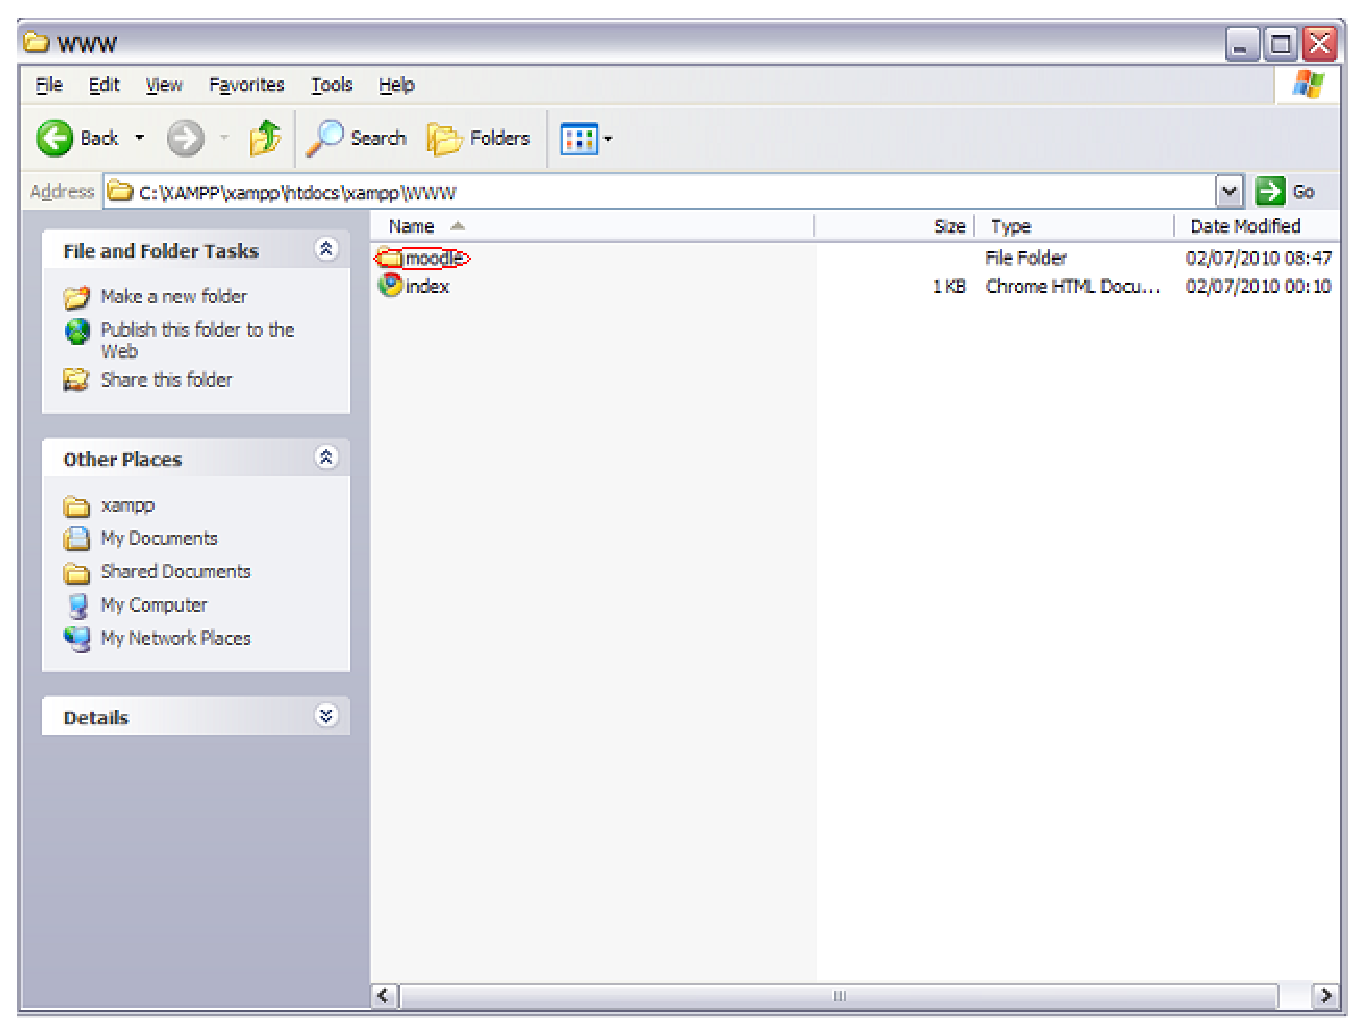
\includegraphics[width=1\textwidth]{char_narzarzedzi//rys//katalog_aplikacji.eps}
\end{figure}
Główny katalog Moodle'a w domyślnej konfiguracji ma nazwę \textit{moodle} \ref{rys:katalog_moodle} i znajdują się w nim podkatalogi i mając nawet nie wielką wiedzę na temat Moodle'a można szybko wywnioskować za co są odpowiedzialne. Na przykład katalog \textit{admin} przechowuje pliki PHP odpowiedzialne za generowanie strony administracyjne. Zaś katalog \textit{lang} przechowuje tłumaczenia interfejsu Moodle'a. Z kolei katalog \textit{mod} przechowuje różne moduły. \\
\begin{figure}[!h]
	\centering
		\caption{Katalog aplikacji Moodle'a} \label{rys:in_moodle}
\end{figure}
		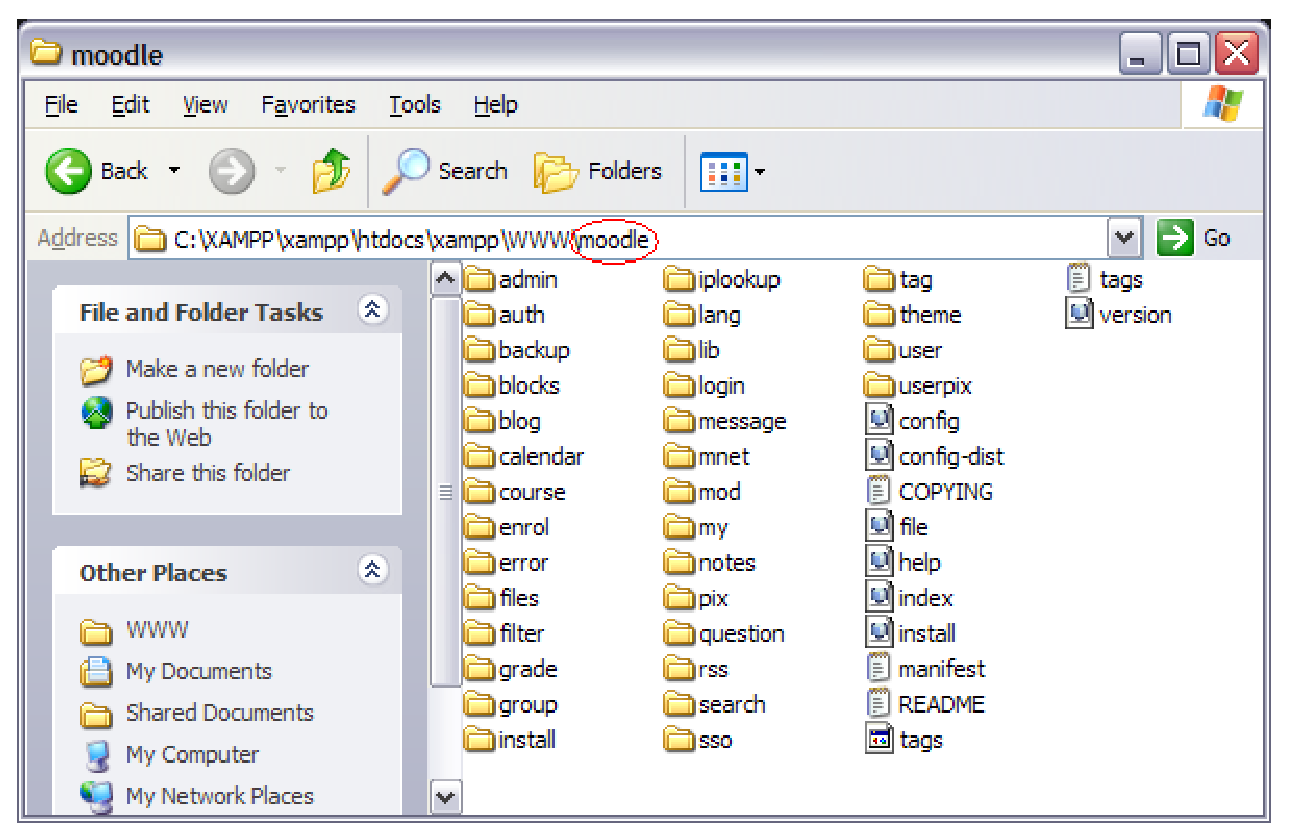
\includegraphics[width=1\textwidth]{char_narzarzedzi//rys//in_moodle.eps}
Rysunek \ref{rys:in_moodle} pokazuje całą zawartość głównego katalogu aplikacji. \\
Ponieważ każdy z podstawowych komponentów i modułów Moodle'a ma swój własny podkatalog. Dzięki temu mogą być one łatwo uaktualniane poprzez zamianę starych plików na nowymi. Dlatego warto sprawdzić co jakiś czas witrynę \href{http://www.moodle.org}{\textit{http://www.moodle.org}} w poszukiwaniu wiadomości o uaktualnieniach i poprawionych błędach. \\
\section{Katalog danych Moodle'a} \label{roz:moodledata}
\begin{figure}[!ht]
	\centering
		\caption{Katalog danych Moodle'a \textit{moodledata}} \label{rys:moodledata}
		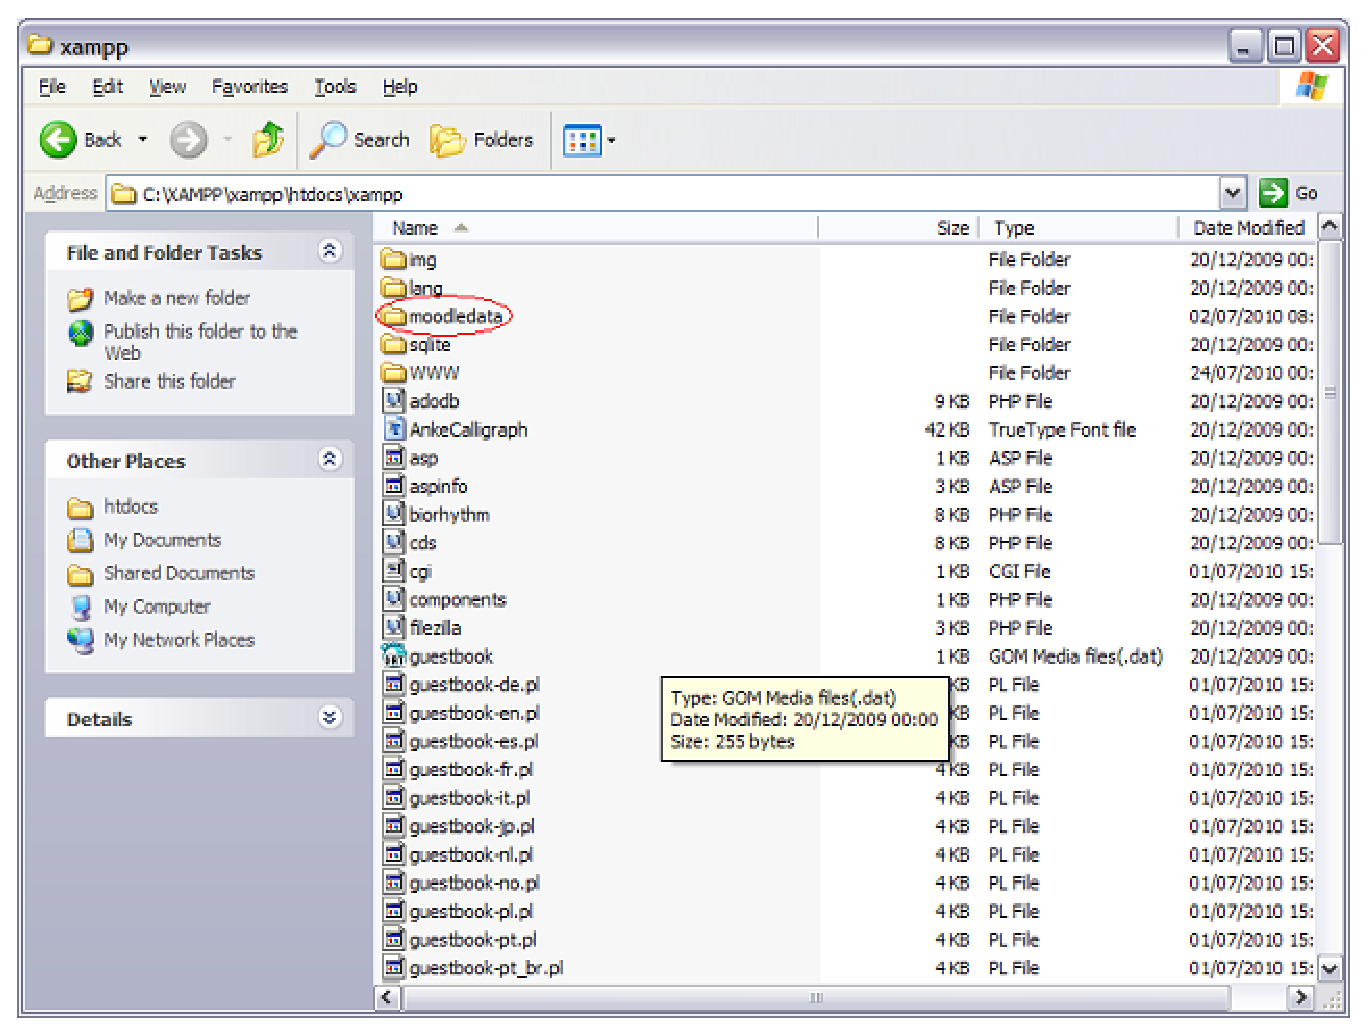
\includegraphics[width=1\textwidth]{char_narzarzedzi//rys//moodledata.eps}
\end{figure}
Wszystkie pliki przesyłane przez użytkowników są przechowywane w katalogu danych Moodle'a. Katalog ten podczas instalacji powinien być umieszczony tak aby nie było do niego dostępu z zewnątrz (internetu). To znaczy że nie powinno być możliwości dostania się do katalogu po wpisaniu jego adresu internetowego w przeglądarce. Są dwa sposoby zabezpieczenia tegoż katalogu. Pierwszy z nich dotyczy pliku \textit{.htaccess}. Zaś drugi, poprzez umieszczenie katalogu poza katalogiem dokumentów publicznych serwera. Jak pokazuje rysunek \ref{rys:moodledata}. Aby zabezpieczyć katalog przed przeglądaniem należy utworzyć w nim plik \textit{.htaccess} i wpisanie doń następujących komend:\\
\hspace{2cm} \texttt{order deny,allow} \\
\hspace{2cm} \texttt{deny from all} \\
\begin{figure}[!hb]
	\centering
		\caption{Wewnątrz katalogu \textit{moodledata}} \label{rys:in_moodledata}
		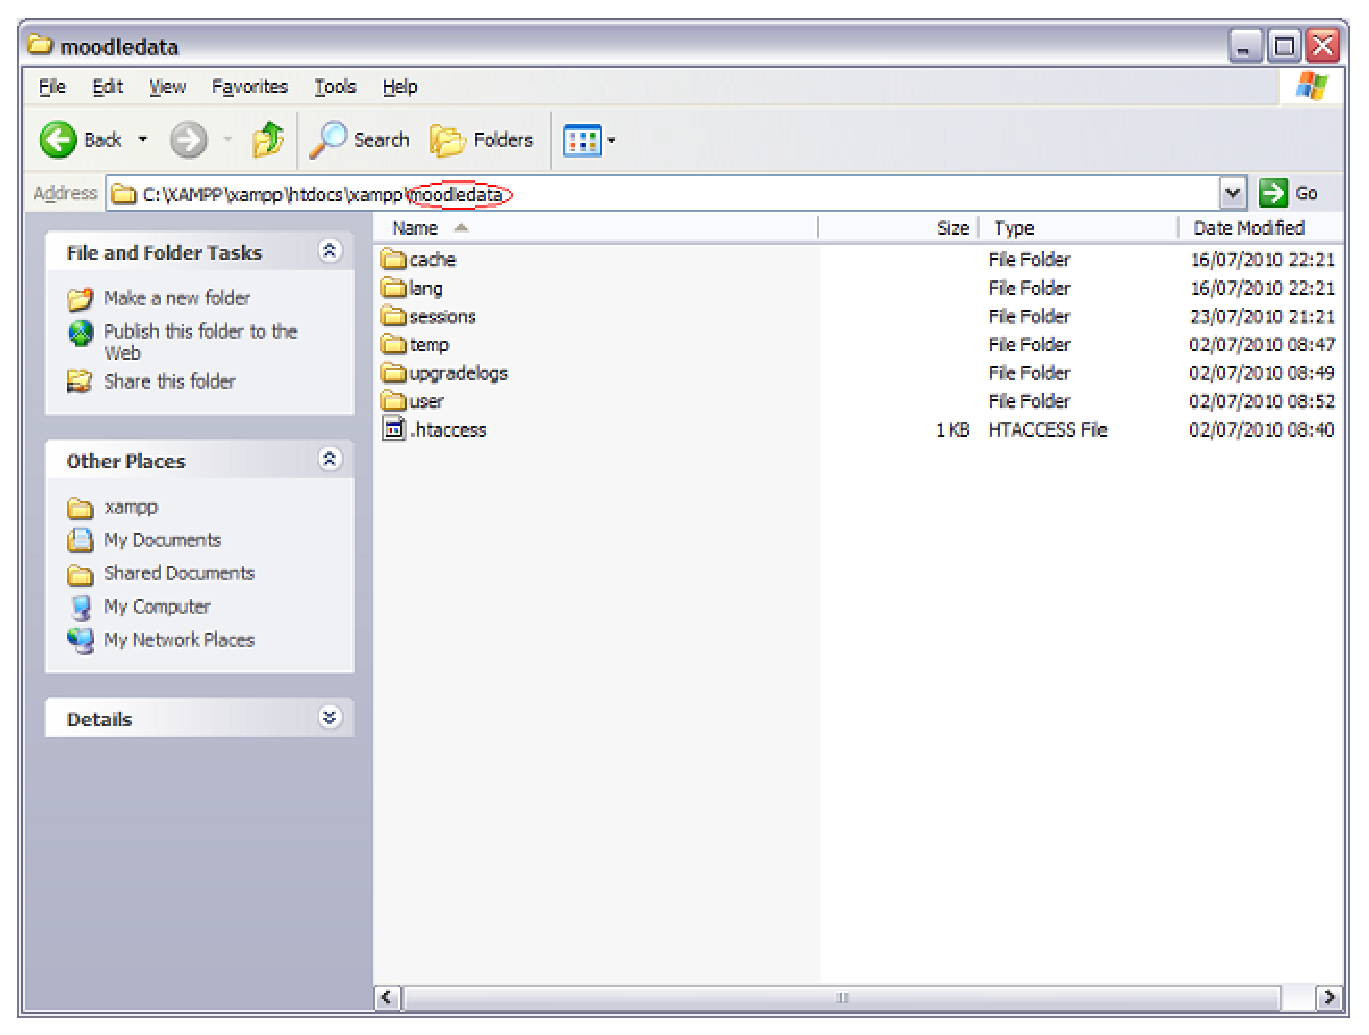
\includegraphics[width=1\textwidth]{char_narzarzedzi//rys//in_moodledata.eps}
\end{figure}
W przykładowej instalacji widać na rysunku\ref{rys:katalog_moodle} katalogiem dokumentów serwera jest \textit{$\backslash$WWW$\backslash$moodle}. Z tego powodu katalog danych został umieszczony poza katalogiem \textit{WWW} i katalogiem \textit{moodle}. Co widać na rysunku \ref{rys:moodledata}. Zaś rysunek \ref{rys:in_moodledata} pokazuje nam zawartość katalogu \textit{moodledata}. Jest tam również umieszczony plik \textit{.htaccess}. \\
\section{Baza danych Moodle'a} \label{roz:baza_dnaych}
\begin{figure}[!ht]
	\centering
		\caption{Kawałek bazy danych Moodle'a} \label{rys:baza}
		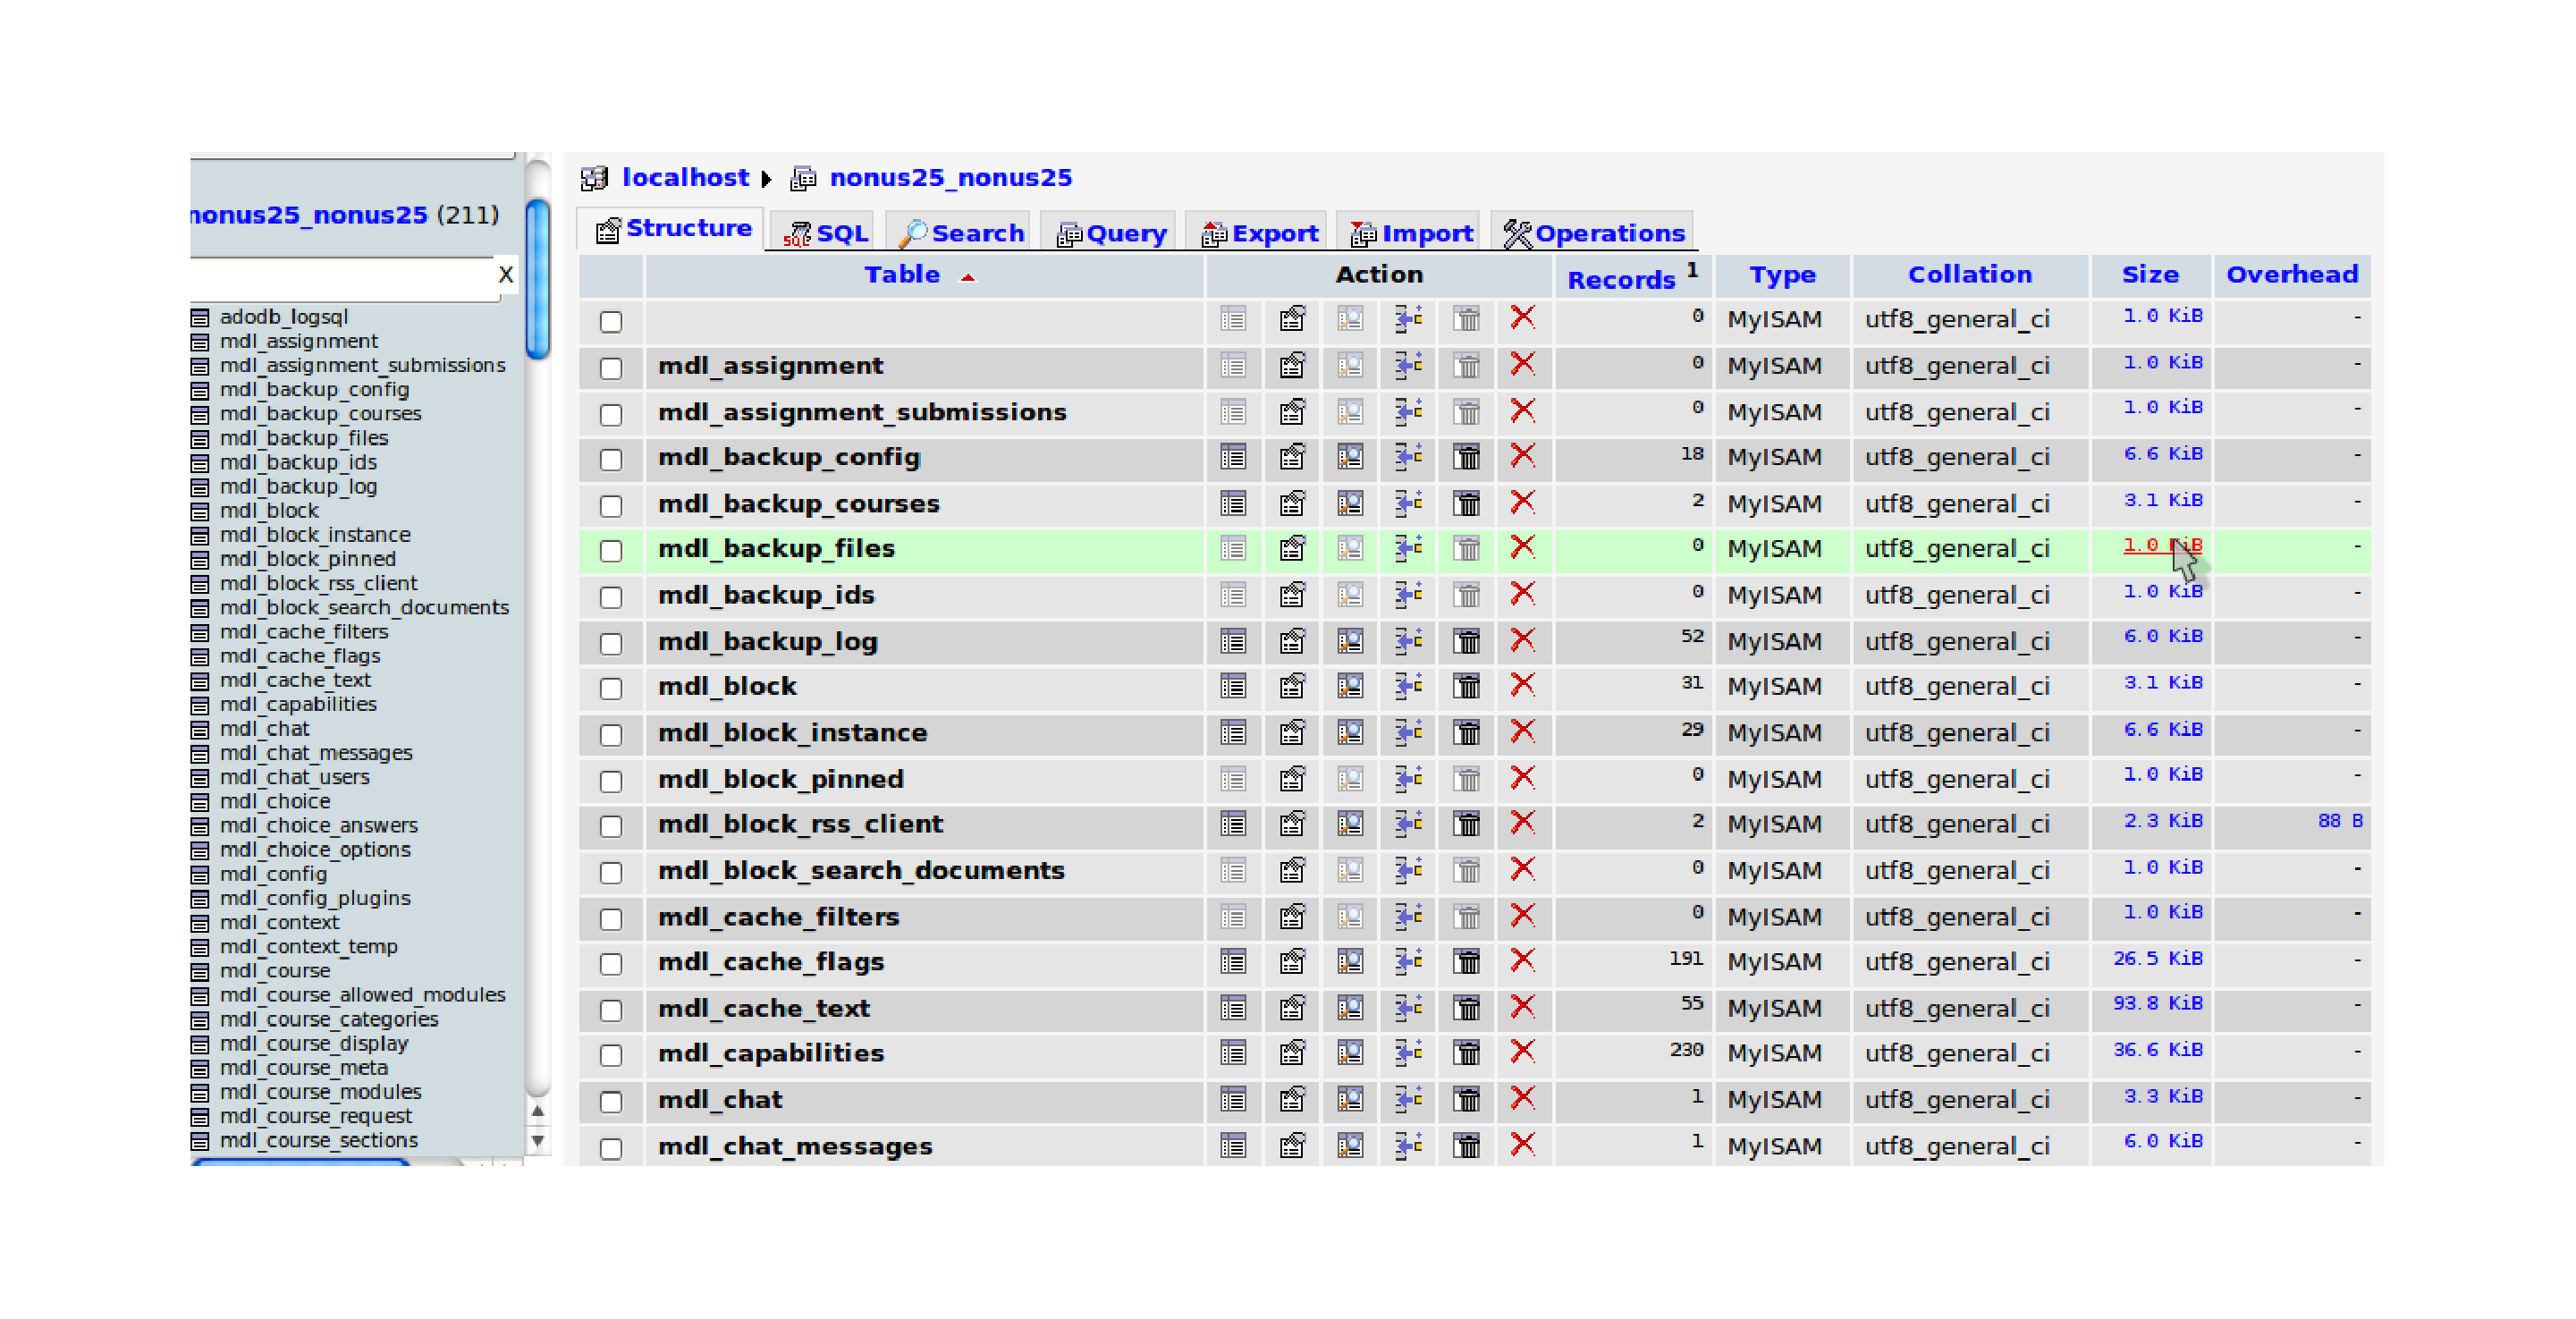
\includegraphics[width=1\textwidth]{char_narzarzedzi//rys//baza.eps}
\end{figure}
Podczas gdy katalog danych Moodle'a przechowuje pliki przesyłane przez użytkowników, bazy danych Moodle'a \ref{rys:baza} przechowują większość obiektów utworzonych za pomocą witryny Moodle'a, są przechowywane w postaci kodu HTML\footnote{HTML~-~język znaczników hipertekstu (ang. HyperText Markup Language} w bazie danych. Odnośniki dodawane do kursów, ustawienia i zawartość forów dyskusyjnych i stron wiki, quizy - wszystko to jest przykładem danych przechowywanych w bazie danych Moodle'a. Pokazuje to rysunek \ref{rys:tabela} \\
\begin{figure}[!hb]
	\centering
		\caption{Tabela \textit{mdl\_course}} \label{rys:tabela}
		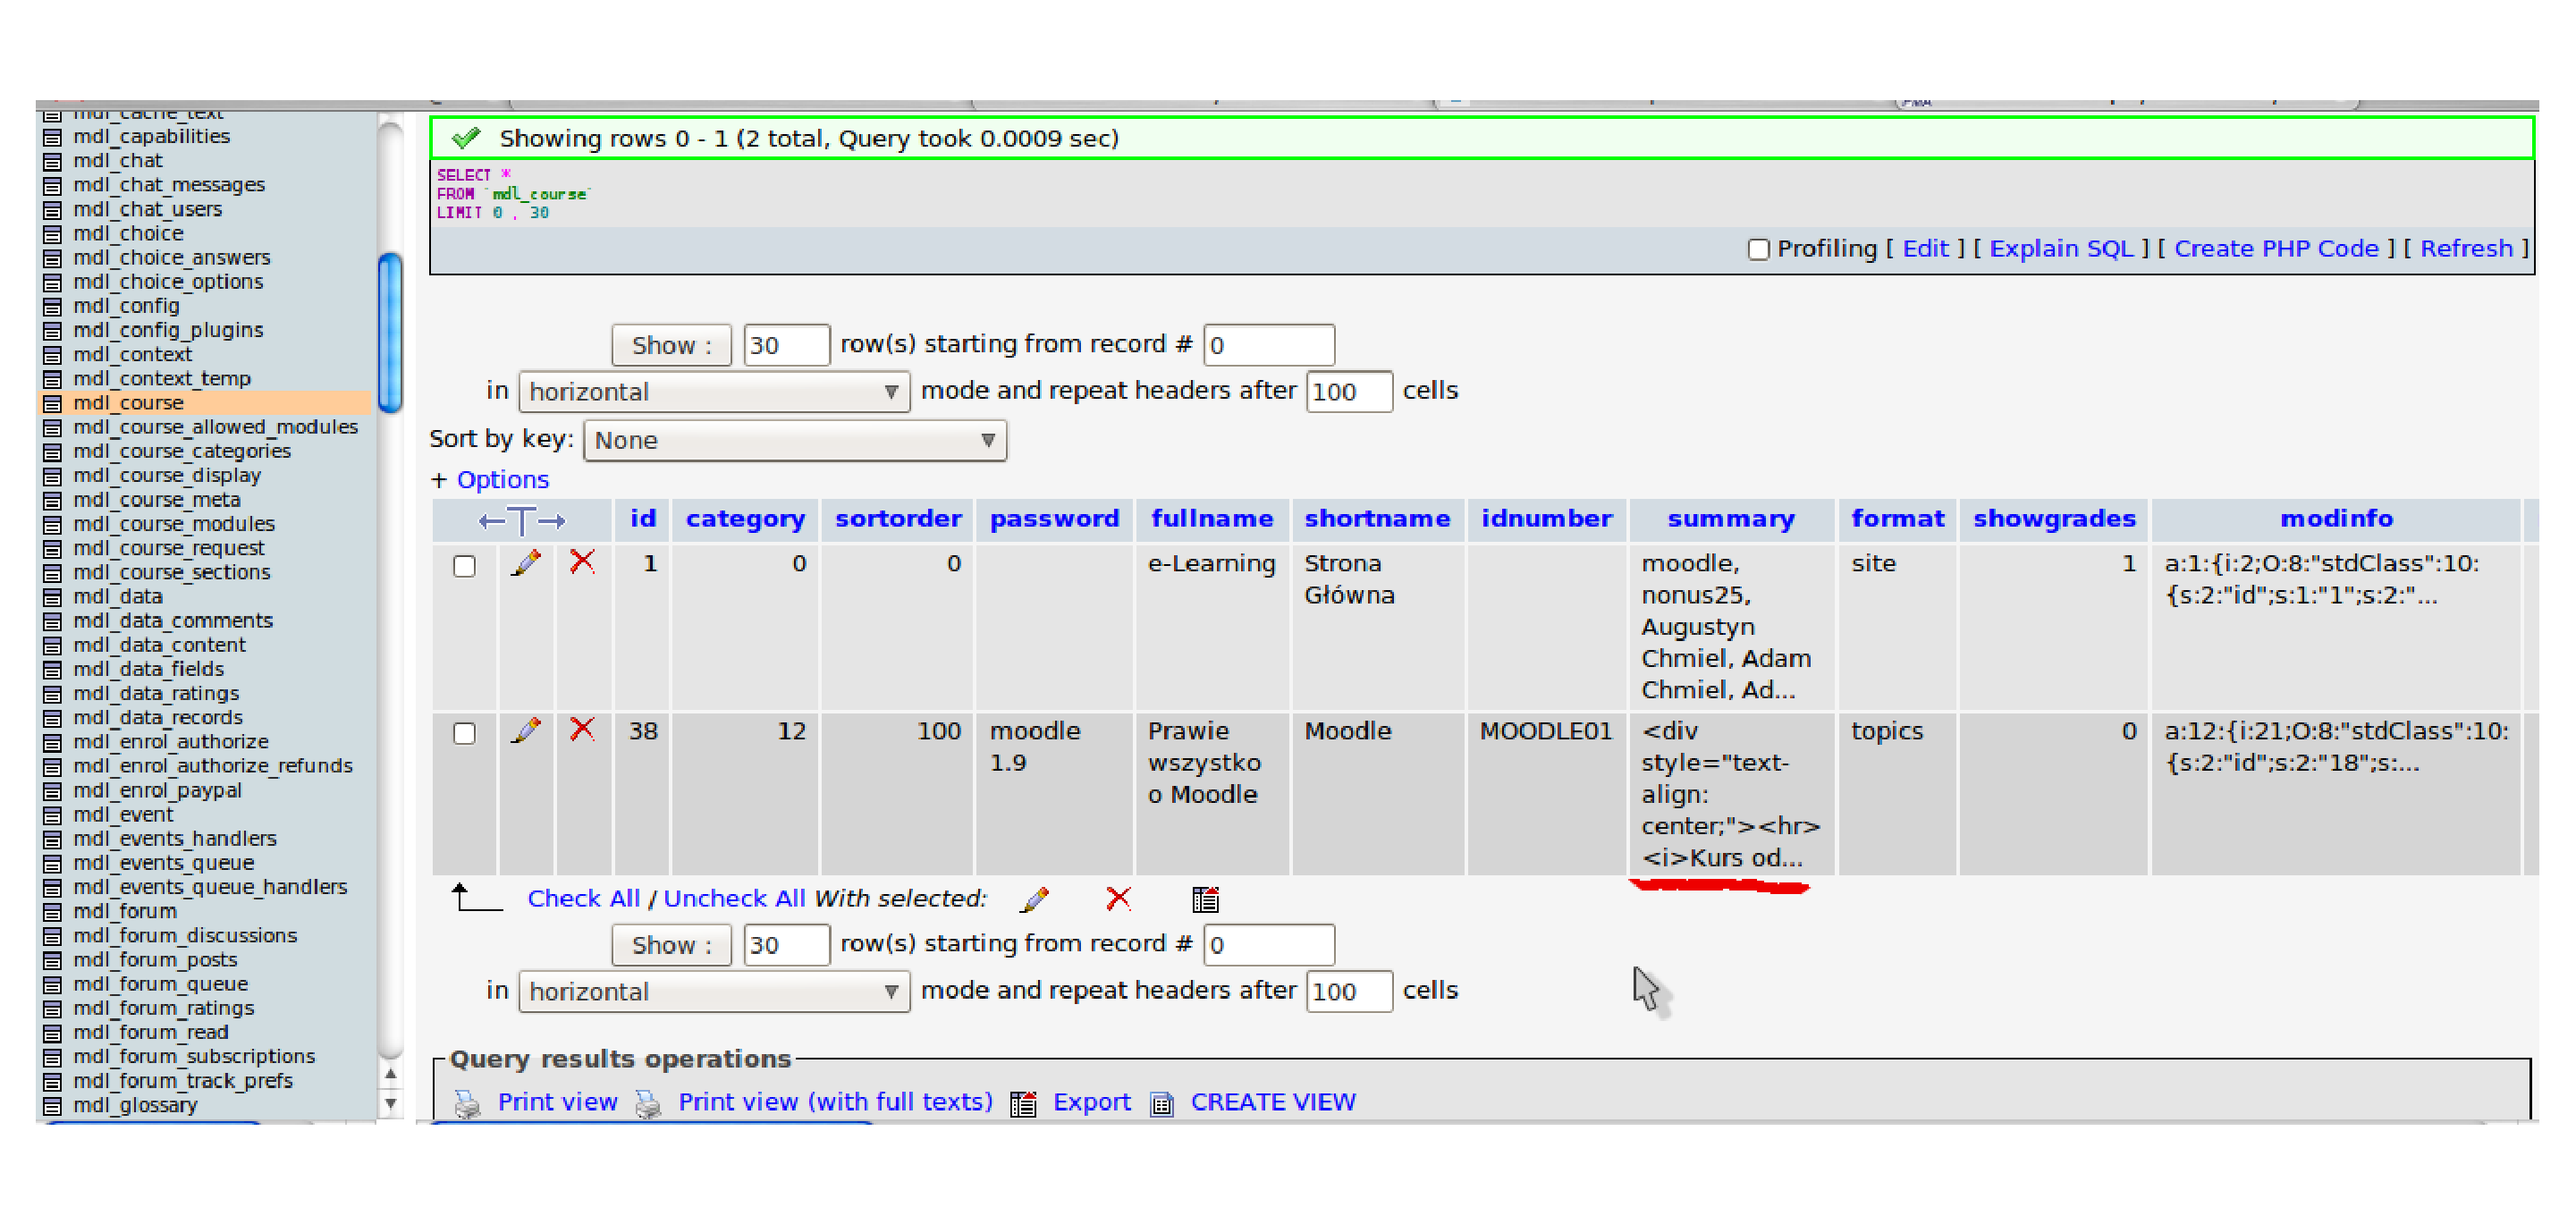
\includegraphics[width=1\textwidth]{char_narzarzedzi//rys//course.eps}
\end{figure}
Trzy części~-~\textbf{katalog aplikacji, katalog danych i baza danych}~-~współpracują ze sobą, tworząc witrynę nauczania. Interfejs w Moodle'u zachęca użytkownika do eksploracji i interakcji pomiędzy uczniami i nauczycielami oraz pomiędzy nimi samymi.\\
\section{Struktura katalogów \textit{Moodle'a}} \label{roz:struktura_moodle}
Aby lepiej zrozumieć strukture aplikacji Moodle'a wymienie i opisze podkatalogi zawarte w katalogu \textit{moodle}: \cite{dokumentacja_moodle}\\
	\begin{itemize}
		\item \textit{config.php}~-~zawiera podstawowe ustawienia. Ten plik nie jest częścią samego Moodle - zostanie utworzony podczas instalacji.
		\item \textit{install.php}~-~skrypt, który uruchomisz w celu utworzenia pliku \textit{config.php}. 
		\item \textit{version.php}~-~określa wersję kodu Moodle 
		\item \textit{index.php}~-~strona główna witryny
		\item \textit{admin/}~-~kod, służący do zarządzania serwerem
		\item \textit{auth/}~-~moduły wtyczek, służących do uwierzytelniania 
		\item \textit{blocks/}~-~moduły wtyczek, służących do obsługi małych bloków tekstowych, znajdujących się z boku wielu stron 
		\item \textit{calendar/}~-~kod, obsługujący zarządzanie i wyświetlanie kalendarzy 
		\item \textit{course/}~-~kod wyświetlający i zarządzający kursami 
		\item \textit{doc/}~-~dokumentacja pomocy Moodle
		\item \textit{files/}~-~kod wyświetlający i zarządzający plikami wysłanymi na serwer 
		\item \textit{lang/}~-~teksty w różnych językach, jeden katalog na język 
		\item \textit{lib/}~-~biblioteki rdzenia kodu Moodle 
		\item \textit{login/}~-~kod do obsługi kont 
		\item \textit{mod/}~-~zawiera wszystkie główne moduły kursów Moodle 
		\item \textit{pix/}~-~podstawowa grafika strony 
		\item \textit{theme/}~-~motywy graficzne/skórki, zmieniające wygląd strony 
		\item \textit{user/}~-~kod wyświetlający i zarządzający użytkownikami 
	\end{itemize}

	\newpage
\chapter{Charakterystyka wykorzystanych technologii} \label{roz:rozdzial_5}
	\thispagestyle{empty}
	\hspace{1cm}Podstawą tworzenia rozwiązań nauczania na odległość jest zapewnienie wymiany informacji pomiędzy prowadzącymi dane zajęcia, a ich odbiorcami. Sprawność wymiany informacji istotnie wpływa na jakość uczenia. Stąd, aby sprawnie prowadzić kształcenie e-learning-owe, konieczne jest dobranie odpowiedniego narzędzia informatycznego, specjalizowanego do tych zastosowań. Wyróżnia się dwie grupy platform dostępnych dla rozwiązań e-learning-owych:
	\begin{itemize}
		\item Platformy open-source, czyli wolne oprogramowanie przystosowane do zdalnego procesu nauczania.
		\item Platformy komercyjne, przeważnie stworzone przez znane firmy komputerowe w celu informatyzacji procesu kształcenia np. \textit{Microsoft Class Server}.
	\end{itemize}
Narzędziem na jaki się zdecydowałem należy do grupy open source. Platforma ta posiada ponad 100~000 zarejestrowanych użytkowników na całym świecie, obsługuje ponad 70 języków. Główna cechą Moodle'a jest modułowość, dzięki czemu interfejs jest łatwy w obsłudze i może się z nim uporać nawet ktoś z niewielką wiedzą informatyczną.\\
Platforma Moodle'a jest obecnie najczęściej używaną platformą zdalnego nauczania. Platforma Moodle'a łączy w sobie dwa systemy CMS\footnote{system zarządzania treścią (ang. Content Management System)} i LMS\footnote{system zarządzania procesem nauczania (ang. Learning Management System)}. Dzięki temu połączeniu cech które posiadają obydwa systemy otrzymano oprogramowanie, które wspomaga realizację procesu nauczania na odległość, pozwala to na umieszczanie oraz zmianę treści w sposób dynamiczny i prosty. \\
\hspace{1cm}Moodle został zaprojektowany przez Martin Dougiamas – doktor nauk pedagogicznych z Curtin University of Technology, Perth, Australia. Dużą zaletą platformy Moodle'a jest jej forma darmowego oprogramowania, gdzie dzięki tej formie Moodle jest platformą która bardzo szybko się rozwija i zwiększa swoją funkcjonalność. Zgodnie z zasadami ruchu open source, system ten jest tworzony przez rzeszę programistów. Każdy może sprawdzić, co zawiera kod systemu, znaleźć błędy i jej poprawić przyczyniając się samemu do rozwoju platformy. Oprogramowanie platformy napisane jest w języku PHP i umożliwia użycie darmowych baz danych (MySQL, PostgreSQL). Platformę można zainstalować w dowolnym środowisku operacyjnym (MS Windows, Unix, Linux).\\
Wymagania dla platformy Moodle'a zostały zawarte w tabeli~\ref{tab:wymagania_sprzetowe} \\
	\begin{table}[!h]
		\centering
		\caption{Wymagania platformy Moodle'a.}
		\label{tab:wymagania_sprzetowe}
		\begin{tabular}{|l|p{10cm}|} \hline
		 & \textbf{Parametry techniczne} \\ \hline
			\textbf{Pamięć RAM:} & minimum 256MB zalecane 1GB. Ogólna zasada mówi ze Moodle może obsługiwać jednocześnie 50 użytkowników na każdy 1GB RAM-u, jednak liczby te mogą uledz zmianie w zależności od sprzętu i oprogramowania. \\ \hline
			\textbf{Przestrzeń dyskowa:} & minimum 160MB wolnego miejsca. Ze względu na materiały do nauczania należy uwzględnić większą ilość wolnego miejsca. \\ \hline
			\textbf{Oprogramowanie:} & Serwer WWW. Głównie Apache'a, ale Moodle powinien działać także pod każdym innym serwerem obsługującym PHP. Interpretator PHP. Dla Moodle w wersji 1.6 lub późniejszej: PHP4 (wersja 4.3.0 lub późniejsza) lub PHP5 (wersja 5.1.0 lub późniejsza). Przyszła wersja Moodle 2.0 i późniejsze nie będą wspierały PHP4 i będą wymagały PHP5 (w wersji 5.2.0 lub późniejszej). Serwer bazodanowy. Dla Moodle 1.7 i późniejszych, MySQL (w wersji 4.1.12 lub późniejszej), PostgreSQL (w wersji 7.4 lub późniejszej) albo Microsoft SQL Server 2005 (w wersji 9 lub SQL Server Express 2005 \\ \hline
		\end{tabular}
	\end{table}
Poza wymaganiami sprzętowymi i programowymi, należy także pomyśleć o objętości instalacji Moodle'a. W znaczeniu ilu użytkowników ma obsługiwać platformę. Najważniejsze w tym przypadku są dwie liczby: \\
	\begin{itemize}
		\item \textbf{Użytkownicy przeglądający} są to tacy użytkownicy, którzy będą mogli przeglądać witrynę.
		\item \textbf{Równocześni użytkownicy bazy} jest to maksymalna liczba użytkowników którzy będą korzystać z bazy danych  
	\end{itemize}
Ogólna zasada dla pojedynczego serwera jest taka, że przybliżona maksymalna ilość użytkowników = RAM (GB) * 50, a przybliżona maksymalna ilość użytkowników przeglądających jest 5 razy większa od poprzedniej wartości. Przykładowo, uniwersytet z 500 komputerami w kampusie i 100 równoległymi użytkownikami potrzebuje 2GB RAM-u na serwerze, aby obsłużyć jednocześnie tylu użytkowników\cite{dokumentacja_moodle}. \\
Platforma Moodle, dzięki budowie modułowej i cechom systemu zarządzania treścią, pozwala na szybkie umieszczanie w niej treści oraz modyfikowanie zawartości strony z danym kursem przez pracowników dydaktycznych, bez konieczności posiadania wiedzy informatycznej. \\
W platformie Moodle wyróżnić można 5 grup użytkowników posiadających różne uprawnienia: \\
	\begin{itemize}
		\item gość~-~może odwiedzić stronę główną platformy, przeglądać opisy, ale nie ma możliwości przystąpienia i przeglądania kursów.
		\item student~-~posiada możliwość przeglądania wybranych kursów, ale jego prawa w kursach są ograniczone.
		\item nauczyciel~bez~praw~edycji~-~mogą uczyć w kursach i oceniać studentów, ale nie mogą wprowadzać zmian edycyjnych.
		\item prowadzący~-~mogą robić wszystko w kursie, np. zmieniać treść czy też oceniać uczniów. Nie mogą natomiast sami tworzyć nowych kursów.
		\item autorzy~kursów~-~mogą tworzyć nowe kursy i być w nich nauczycielami oraz przypisywać do kursów prowadzących.
		\item administrator~-~mogą robić wszystko z kursami jak i również z całą platformą.
	\end{itemize}
Studenci sami tworzą swoje konta. Administrator oraz wyznaczeni przez niego autorzy kursów kontrolują tworzenie kursów i przyporządkowują do nich prowadzących. Dla ograniczenia dostępu do danego kursu, możliwe jest ustanowienie do niego hasła dostępowego. Prowadzący kurs mogą: zapisywać i wypisywać studentów uczestniczących w tym kursie oraz umieszczać treści dydaktyczne. \\
Tworzony kurs może posiadać trzy formaty: \\
	\begin{itemize}
		\item towarzyski
		\item tematyczny
		\item tygodniowy
	\end{itemize}
Wprowadzany tekst jest umieszczany za pomocą edytora WYSIWIG\footnote{WYSIWIG~-~co znaczy dosłownie To Co Widzisz Jest Tym Co Otrzymasz (ang. What You See Is What You Get)} HTML\footnote{HTML~-~język znaczników hipertekstu (ang. HyperText Markup Language)}. Prowadzący kurs ma do wykorzystania duży zestaw narzędzi wspomagających, takich jak:\\
	\begin{itemize}
		\item ankiety
		\item quizy
		\item zadania 
		\item fora 
		\item dzienniki itd.
	\end{itemize}
Posiada również dostęp do monitoringu logowania aktywności studentów. Prowadzący dokonuje ocen prac studentów za pośrednictwem platformy i może także przesłać informacje zwrotne. Platforma również posiada czat, który umożliwia prowadzenie rozmów w czasie rzeczywistym między studentami i prowadzącymi kurs. Platforma ta umożliwia również umieszczanie treści w postaci multimedialnej (audio, wideo itp.), co znacznie wzbogaca przekazywanie wiadomości i czyni je bardziej przystępnymi\cite{nowakowski}. 

	\newpage
\chapter{Uzasadnienie wyboru narzędzi} \label{roz:rozdzial_6}
	\thispagestyle{empty}
	\hspace{1cm} Przy wyborze narzędzia do tworzenia witryny wspomagającej zdalne nauczanie brałem pod uwagę następujące czynniki, które teraz wymieniem i pokrótce opisze:
	\begin{itemize}
		\item popularność
		\item koszt wykonania witryny
		\item społeczność
		\item skutecznością w realizowaniu celów dydaktycznych
	\end{itemize} 
\section{Popularność} \label{roz:popularnosc_moodle}
\hspace{1cm}  Obecnie najbardziej popularną platformą open source jest platforma Moodle'a. Platforma jest najbardziej znana i najczęściej instalowana do nauczania przez Internet. Jest ona prosta w obsłudze, bogata w funkcje. Zbudowana jest na solidnej filozofii edukacyjnej i ma ogromną społeczność, która wspiera i rozwija platformę. Może śmiało konkurować z wielkimi komercyjnymi serwisami w zakresie zestawów funkcji i jest łatwy do rozszerzenia. Stąd tak duża popularność tej że platformy.
\section{Koszt wykonania witryny} \label{roz:koszt}
\hspace{1cm} Koszt postawienia nie wielkiej platformy Moodle'a jest równy zeru. Projekt jest jak już wcześniej pisałem open source. Dla osób które wcześniej nie spotkały się z z tego typu sformułowaniem jest trudne do zrozumienia jak potężna jest ta idea, i jak zmieniła świat programistów. Pomysł sam w sobie jest prosty: \textit{open source} oznacza, że użytkownicy mają dostęp do źródła kodów platformy. Każdy użytkownik może zaglądać do kodów i modyfikować je na swój własny sposób. Więc czemu jest to tak ważne ? Każdy może pobrać i używać Moodle za darmo, użytkownicy mogą tworzyć nowe moduły, funkcje, naprawiać bugi, poprawiać wydajność, lub po prostu uczyć się jak inni ludzie rozwiązują programistyczne problemy. Moodle może zostać zainstalowany na każdym serwerze obsługującym PHP i umożliwia użycie darmowych baz danych (MySQL, PostgreSQL itp.). Prawie każdy serwer spełnia te warunki.
\section{Społeczność} \label{roz:spolecznosc}
Moodle posiada bardzo dużą i aktywną społeczność, są to osoby które używają Moodle'a jak i zarówno osoby, które tworzą nowe funkcje i udoskonalenia. Każdy ma dostęp do tej społeczności pod adresem \href{http://moodle.org/}{moodle.org} jak również zapisać się na kurs korzystania z Moodle. Można tam znaleźć ludzi którzy są skłoni pomóc nowym użytkownikom w postawieniu i uruchomieniu platformy, w rozwiązywaniu problemów i przy efektywnym używaniu Moodle. Na obecną chwile na \href{http://moodle.org/}{moodle.org} jest zarejestrowanych 300,000 użytkowników i ponad 30,000 stron w 195 krajach. Ta społeczność ma również wkład w przetłumaczeniu platformy na ponad 70 języków. Moodle zawdzięcza tak duże sukcesy właśnie dzięki tak dużej społeczności, gdzie zawsze znajdzie się ktoś kto ma odpowiedz na pytanie lub ktoś kto służy radą. 
\section{Filozofia edukacji} \label{roz:fil_edu} 
\hspace{1cm} Większość CMS-ów była budowana wokół narzędzi, nie pedagogiki. Zarówno większość komercyjnych CMS-ów była również budowana mając na uwadze same narzędzia, gdzie Moodle zostało zaprojektowane i budowane z myślą skutecznego uczenia. Konstruktywizm społeczny jest oparty na założeniu, że ludzie uczą się najlepiej, gdy są zaangażowani w społecznym procesie konstruowania wiedzy poprzez akt budowy materiałów dla innych. Określenie proces społeczny oznacza, że uczenie się jest to coś, co robimy w grupach. \\
Można stwierdzić, że kształcenie na odległość, realizowane w systemie Moodle jest technologią pedagogiczną. Poniżej przedstawiona zostanie tabela\ref{tab:pedagogika}~\ref{tab:cd_pedagogika}~\ref{tab:cd1_pedagogika} (źródło:\cite{pedagogika}) ilustruje potwierdzenie tego założenia.
	\begin{table}[!h]
		\centering
		\caption[Analiza technologii pedagogicznej w Moodle'u]{Analiza technologii pedagogicznej kształcenia na odległość na podstawie wykorzystania systemu MOODLE}
		\label{tab:pedagogika}
		\begin{tabular}{|p{4cm}|p{4cm}|p{9cm}|} \hline
			 \textbf{Charakterystyka technologii pedagogicznej} & \textbf{Opis} & \textbf{Opis technologii pedagogicznej
kształcenia na odległość na podstawie
wykorzystania systemu MOODLE} \\ \hline
			identyfikacja & & \\ \hline
			nazwa technologii & nazwa technologii & technologia pedagogiczna kształcenia na odległość na podstawie wykorzystania systemu MOODLE \\ \hline
			konceptualna część (opis idei, hipotez, zasad technologii) & docelowe założenia i orientacje; podstawowe idee i zasady; pozycja uczącego się w procesie kształcenia & wspomaganie nowych stylów nauki, przede wszystkim kognitywnego, kreatywnego i konstruktywistycznego [Piaget, Papert, Juszczyk, Kwiecicki, Le Blank, Dewey, Bruner, Wygotski], w tym ułatwienie różnych form komunikacji i grupowych form nauki, wzajemnej oceny, kierowania uczniami, także możliwość prostej zamiany ról: uczeń – nauczyciel – twórca (materiałów dydaktycznych) kursów dystansowych. Uczący się ma możliwość samodzielnego konstruowania swojej nauki (czas, miejsce, tempo, treści merytoryczne, tematy projektów), jest aktywna strona procesu nauczania. \\ \hline
		właściwości zawartości kształcenia & orientacja na osobowe struktury (WUN – wiedza, umiejętności, nawyki);\newline objętość i charakter kształcenia, dydaktyczna struktura planu szkolnego, materiału, programów, formy przedstawienia & orientacja na struktury osobowe (WUN), jak również na rozwój umiejętności samodzielnej nauki;\newline objętość i charakter kształcenia zależą od celów nauki, adresata, charakteru przedmiotowego obszaru, przygotowania uczniów itd.;\newline dydaktyczna struktura szkolnego planu, materiału, programów – modułowa;\newline forma przedstawienia – multimedialna, hipertekstowa. Uczący się posiada ciągły dostęp do wszystkich zasobów edukacyjnych \\ \hline
		\end{tabular}
	\end{table}

	\begin{table}[!h]
		\centering
		\caption[c.d. Analiza technologii pedagogicznej w Moodle'u]{Analiza technologii pedagogicznej kształcenia na odległość na podstawie wykorzystania systemu MOODLE}
		\label{tab:cd_pedagogika}
		\begin{tabular}{|p{4cm}|p{4cm}|p{9cm}|} \hline
			\textbf{Charakterystyka technologii pedagogicznej} & \textbf{Opis} & \textbf{Opis technologii pedagogicznej
kształcenia na odległość na podstawie
wykorzystania systemu MOODLE} \\ \hline
			charakterystyka procesowa & właściwości metodyki, zastosowania metod i środków nauki; charakterystyka motywacyjna; organizacyjne formy procesu kształcenia; zarządzanie procesem kształcenia (diagnostyka, projektowanie, regulamin, korekcja); kategoria uczniów, dla których została opracowana technologia & zastosowanie kreatywnych metod nauki \newline– metoda projektów, nauka we współpracy, portfoliów ucznia, metoda problemowa, burza mózgów, forum itd.;\newline środki nauczania – elektroniczne, hipertekstowe, multimedialne materiały, cięgle dostępne na serwerze platformy nauki zdalnej;\newline – motywacja jest osiągniecie celu nauczania przez elastyczne formy, metody, aktualne i ujmujące środki i zasoby, różnorodne formy kontaktu i współdziałania;\newline – organizacyjne formy procesu kształcenia;\newline – lekcja, seminarium, forum, samodzielna praca z zasobami, tekstami, forum, dziennikiem itd.;\newline – zarządzanie procesem nauczania odbywa się przez różne dostępne dla wykładowcy narzędzia: \newline projektowanie – scheduler, struktura kursów, format kursów; \newline diagnostyka – oceny, wiadomości, forum, dialog, automatyczne kopie e-mail, możliwość eksportu ocen do Excela; \newline administrowanie – zbieranie oraz przechowywanie danych o obecności, aktywności, oceny, scheduler, logi, analiza logów, RSS, tworzenie i zarządzanie grupami, poziom praw dostępu; \newline ewaluacja – kwestionariusz, ankieta, głosowanie, logi, dziennik itd. Technologia przewiduje udział w nauce różnych kategorii użytkowników w zależności od celów kształcenia\\ \hline
		\end{tabular}
		\end{table}
		\begin{table}[!h]
		\centering
		\caption[c.d. Analiza technologii pedagogicznej w Moodle'u]{Analiza technologii pedagogicznej kształcenia na odległość na podstawie wykorzystania systemu MOODLE}
		\label{tab:cd1_pedagogika}
		\begin{tabular}{|p{4cm}|p{4cm}|p{9cm}|} \hline
			\textbf{Charakterystyka technologii pedagogicznej} & \textbf{Opis} & \textbf{Opis technologii pedagogicznej
kształcenia na odległość na podstawie
wykorzystania systemu MOODLE} \\ \hline
			zabezpieczenie programowo-metodyczne & plany i programy nauczania;\newline podręczniki i poradniki metodyczne;\newline materiały dydaktyczne;\newline poglądowe techniczne środki nauczania;\newline instrumentarium diagnostyczne & plany i programy nauczania zdalnych
kursów są opracowane przez nauczycieli wykładowców w zależności od przedmiotowego obszaru, wieku uczniów, ich poziomu przygotowania, celów nauki, charakteru szkolnego materiału itd. Plany i programy nauczania zdalnych kursów, jak również ich szczegółowy opis i komentarz, publikuje się na serwerze;\newline materiały dydaktyczne i poradniki metodyczne – w formie elektronicznej, hipertekstowej, multimedialnej; \newline odwołanie się do zasobów Internetu, słowniki tematyczne, cały czas dostępne na serwerze z systemem MOODLE (lekcje, słowniki, zasoby, pliki, linki, katalogi, wiki itd.) \\ \hline
			kryteria oceny technologii pedagogicznej & efektywność; \newline skuteczność & analiza i ocena efektywności i skuteczności
w postaci aktywności, posterów w uczeniu się uczniów (kontrola bieżąca i końcowa), samo i wzajemnej oceny przez uczniów swoich osiągnięcie nauczania odbywa się za pomocą różnorodnych narzędzi, dostępnych w systemie MOODLE:\newline
obecność, aktywność, oceny, Scheduler, logi, analiza logów, RSS, grupy, poziom praw dostępu, komentarze, dziennik, testy, Hot Potatoes Quiz, zadania, lekcja, obecność, aktywność, logi, słownik, seminaria, oceny, obrona projektów (indywidualnych i grupowych), wiadomości, omówienie na forum, możliwość eksportu ocen do Excela, kwestionariusz, ankieta, badanie (głosowanie) itd. \\ \hline
		\end{tabular}
		\end{table}
\textbf{Technologia indywidualizacji nauczania} źródło:\cite{pedagogika}
Indywidualizacja nauczania – forma, model organizacji procesu nauczania-uczenia się, przy którym: \\
	\begin{itemize}
		\item nauczyciel współdziała tylko z jednym uczniem;
		\item jeden uczeń współdziała tylko ze środkami nauczania.
	\end{itemize}
Indywidualne podejscie to:\\
	\begin{itemize}
		\item zasada pedagogiki, zgodnie z która w procesie pracy dydaktyczno-wychowawczej z grupa nauczyciel współdziała z poszczególnymi uczniami według indywidualnego modelu, uwzględniając ich szczególne cechy;
		\item orientacja na indywidualne właściwości uczącego się w kontakcie z nim;
		\item uwzględnienie indywidualnych właściwości uczącego się w procesie nauczania-uczenia się.
	\end{itemize}
Zalety indywidualnego nauczania w tradycyjnej nauce i w kształceniu na odległość z użyciem Moodle przedstawia tabela \ref{tab:indywidualnego} \ref{tab:cd_indywidualnego}, źródło:\cite{pedagogika}
		\begin{table}[!h]
		\centering
		\caption[Indywidualizacja nauczania]{Indywidualizacja nauczania-uczenia się w systemie tradycyjnym i systemie kształcenia na odległość z wykorzystaniem systemu MOODLE}
		\label{tab:indywidualnego}
		\begin{tabular}{|p{4cm}|p{5.5cm}|p{7.5cm}|} \hline
			\textbf{zalety nauczania indywidualnego} & \textbf{warunki realizacji indywidualnego podejścia w nauczaniu tradycyjnym} & \textbf{indywidualizacja nauczania w kształceniu na odległość z wykorzystaniem systemu CLMS MOODLE} \\ \hline
		pozwala całkowicie adaptować zawartość, metody i tempo naukowej działalności uczącego się do jego poziomu i możliwości & proces pracochłonny i trudny do zrealizowania w systemie tradycyjnym: klasowo-lekcyjnoprzedmiotowym & w systemie MOODLE zawartość, metody i tempo szkolnej działalności uczącego się można dostatecznie łatwo, szybko i efektywnie adaptować do jego poziomu i możliwości, dzięki giętkiemu systemowi ustawień i parametrów; można zmienić format kursu, strukturę, jego zawartość i stosowane metody \\ \hline
		pozwala śledzić każde działanie uczącego się i wykonywane operacje przy rozwiązywaniu konkretnych zadań & proces trudny, prawie niewykonalny dla realizacji w systemie tradycyjnym klasowo-lekcyjnym z powodu braku niezbędnych mechanizmów i narzędzi, jak również z powodu wciąż dużej liczby uczniów w jednej klasie & w systemie MOODLE dostępne jest całe spektrum pożytecznych i efektywnych mechanizmów, pozwalających śledzić aktywność ucznia, jego osiągnięcia, realizacje tych lub innych zadań i odpowiedzi na testy, urzeczywistniać pełny monitoring pracy z danym kursem nauczania, co może pomóc w zbudowaniu i korekcji indywidualnej drogi nauczania danego uczącego się \\ \hline
		pozwala śledzić jego osiągnięcia od braku wiedzy do wiedzy & proces śledzenia osiągnięć ucznia od braku wiedzy do wiedzy ma ograniczone możliwości & śledzenie osiągnięć ucznia w systemie MOODLE jest permanentne i wszechstronne, rezultaty mogą być przedstawione w różny sposób: w postaci tabeli, wykresu, w punktach, w procentach na tle poprzednich rezultatów danego ucznia albo na tle klasy \\ \hline
		\end{tabular}
		\end{table}

		\begin{table}[!h]
		\centering
		\caption[c.d. Indywidualizacja nauczania ]{Indywidualizacja nauczania-uczenia się w systemie tradycyjnym i systemie kształcenia na odległość z wykorzystaniem systemu MOODLE}
		\label{tab:cd_indywidualnego}
		\begin{tabular}{|p{4cm}|p{5.5cm}|p{7.5cm}|} \hline
			\textbf{zalety nauczania indywidualnego} & \textbf{warunki realizacji indywidualnego podejścia w nauczaniu tradycyjnym} & \textbf{indywidualizacja nauczania w kształceniu na odległość z wykorzystaniem systemu CLMS MOODLE} \\ \hline
			pozwala wnosić w porę niezbędne korekcje do działalności, zarówno uczącego się, jak i nauczyciela & procedura jest bardzo utrudniona z powodu braku sprzężenia zwrotnego i współdziałania miedzy uczącym się a nauczycielem & dzięki giętkiej i elastycznej strukturze modułowej i koncepcji funkcjonowania, system MOODLE, opiera się na zasadach konstruktywizmu, uwzględniając i realizując idee pedagogiki kognitywnej i częściowo nauczania programowanego; pozwala w każdej chwili wnosić niezbędne korekty do kursu, jak również do działalności zarówno uczącego się, jak i nauczyciela; \\ \hline
		pozwala przysposabiać ich do wciąż zamieniającej się, lecz kontrolowanej sytuacji ze strony nauczyciela oraz ucznia & ten proces powinien był być ściśle związany ze stałym monitoringiem procesu nauczania uczenia się i jego rezultatów, ich analizy, które w nauczaniu tradycyjnym osiągnięte praktycznie być nie może & w systemie istnieje obiektywny permanentny monitoring wszystkich odbywających się procesów, tak na poziomie ucznia(ów), jak i na poziomie nauczyciela(i): logi, aktywność, długotrwałość sesji, rezultaty nauczania, komentarze ze strony nauczyciela, kolegów, wykorzystanie tych lub innych zasobów, narzędzi dla kontroli (samokontroli), prośba o pomoc do nauczyciela lub kolegów w grupie itd.; w zależności od otrzymanych danych nauczyciel w każdej chwili może wnieść zmiany w proces nauczania-uczenia się \\ \hline
		\end{tabular}
		\end{table}

	\newpage
\chapter{Projekt systemu} \label{roz:rozdzial_7}
	\thispagestyle{empty}
	\section{Charakterystyka witryny} \label{roz:charakterystyka}
\hspace{1cm} Podczas tworzenia witryny jak już wcześniej pisałem skorzystam z systemu komputerowego który pozwala organizować i wspomagać nauczanie przez Internet. Systemy takie nazywa się platformami edukacyjnymi określamy je również skrótem LMS\footnote{LMS~-~ang. Learning Management System}. Platforma Moodle'a reprezentuje właśnie tą grupę systemów, które mają głównie za zadanie: \\
	\begin{itemize}
		\item gromadzenie maeriałów dydaktycznych
		\item ich organizowaniu
		\item udostępnianiu 
	\end{itemize}
\ \\
\textbf{Gromadzenie} \\
Wszystkie materiały dydaktyczne jakie będą lub też mogą być utworzone będą wchodziły w skład platformy. Materiały można tworzyć w innych systemach, a później przesyłać je na platformę. Jednakże Moodle jest wyposażony we własne edytory tekstów, grafiki, stron internetowych i z dużym powodzeniem można z nich korzystać, by tworzyć materiały bezpośrednio na platformie. Dodatkowo Moodle posiada własny zestaw narzędzi do tworzenia różnorodnych ćwiczeń i aktywności dla uczniów. Przy pomocy tych narzędzi można tworzyć na platformie ciekawe testy, quizy, kursy czy inne zadania. Kurs zaprezentowany na witrynie będzie zawierał materiały utworzone przy pomocy tych narzędzi. Materiały zgromadzone na platformie będą po części napisane przezemnie jak równierz będą zamieszczone odnośniki do materiałów znalezionych w Internecie. Materiał bedzie przechowywany w postaci stron internetowych, stron tekstowych, plików pdf, i odnośników do innego źródła wiedzy. \\
\\
\newpage
\ \\
\textbf{Organizacja} \\
Aby sensownie móc korzystać ze zgromadzonych materiałów należy je odpowiednio poukładać w większe lub mniejsze jednostki dydaktyczne~-~\textit{kursy}. Moodle pozwala utworzyć taki kurs, odpowiednio zaprojektować jego budowę. Kurs znajdujący się na witrynie używa do organizacji układu tematycznego gdzie cały materiał jest odzielony na trzy tematy. Dostęp do którego kolwiek tematu będzie dowolny i nie będzie wymuszał na uczniu kolejnosci w przeglądaniu treści kursu.\\
\\
\textbf{Udostępnianie} \\
Moodle pozwala dokładnie określić, kto będzie posiadał dostęp do określonych materiałów i w jakim czasie. Uczeń Który uzyskał dostęp do kursu może pobierać przeznaczone dla niego materiały, wykonywać ćwiczenia i zgłaszać swoje rozwiązania. Nauczyciel posiada wgląd w informacje o pracy ucznia i jego rozwiazaniach. Następnie nauczyciel może je poddać ocenie i/lub skomentować. Kurs wchodzący w skła projektu posiada forme wolną, czyli nikt nie będzie oceniany po skorzystaniu z kursu. Dostęp do kursu będą posiadać wszyscy zarejestrowani użytkownicy.\\
\\
\\
\ Celem tego kursu będzie szybkie zapoznanie i wprowadzenie użytkownika z platformą Moodle'a. Każdy użytkownik po przejżeniu materiałów powinen wiedzieć co to jest Moodle, być zdolny samodzielnie zainstalować platformę oraz w razie potrzeby dodać jakiś dodatkowy moduł do Moodla'a. Wykonać prostą konfigurację witryny jak i poźniej umieć nią zarządzać.

\section{Opis działania witryny} \label{roz:opis}
Wejście na stronę platformy MOODLE znajdować się będzie pod adresem \\ \href{http://moodle.chmielua.fazz.pl}{\textit{http://moodle.chmielua.fazz.pl}}. Po wejściu w adres, zostajemy przeniesieni do strony o adresie \href{http://moodle.chmielua.fazz.pl/login/index.php}{\textit{http://moodle.chmielua.fazz.pl/login/index.php}} dostaniemy panel logowania do witryny Moodle'a rys.\ref{rys:login}. 
\begin{figure}[!h]
	\centering
		\caption{Logowanie do witryny} \label{rys:login}
		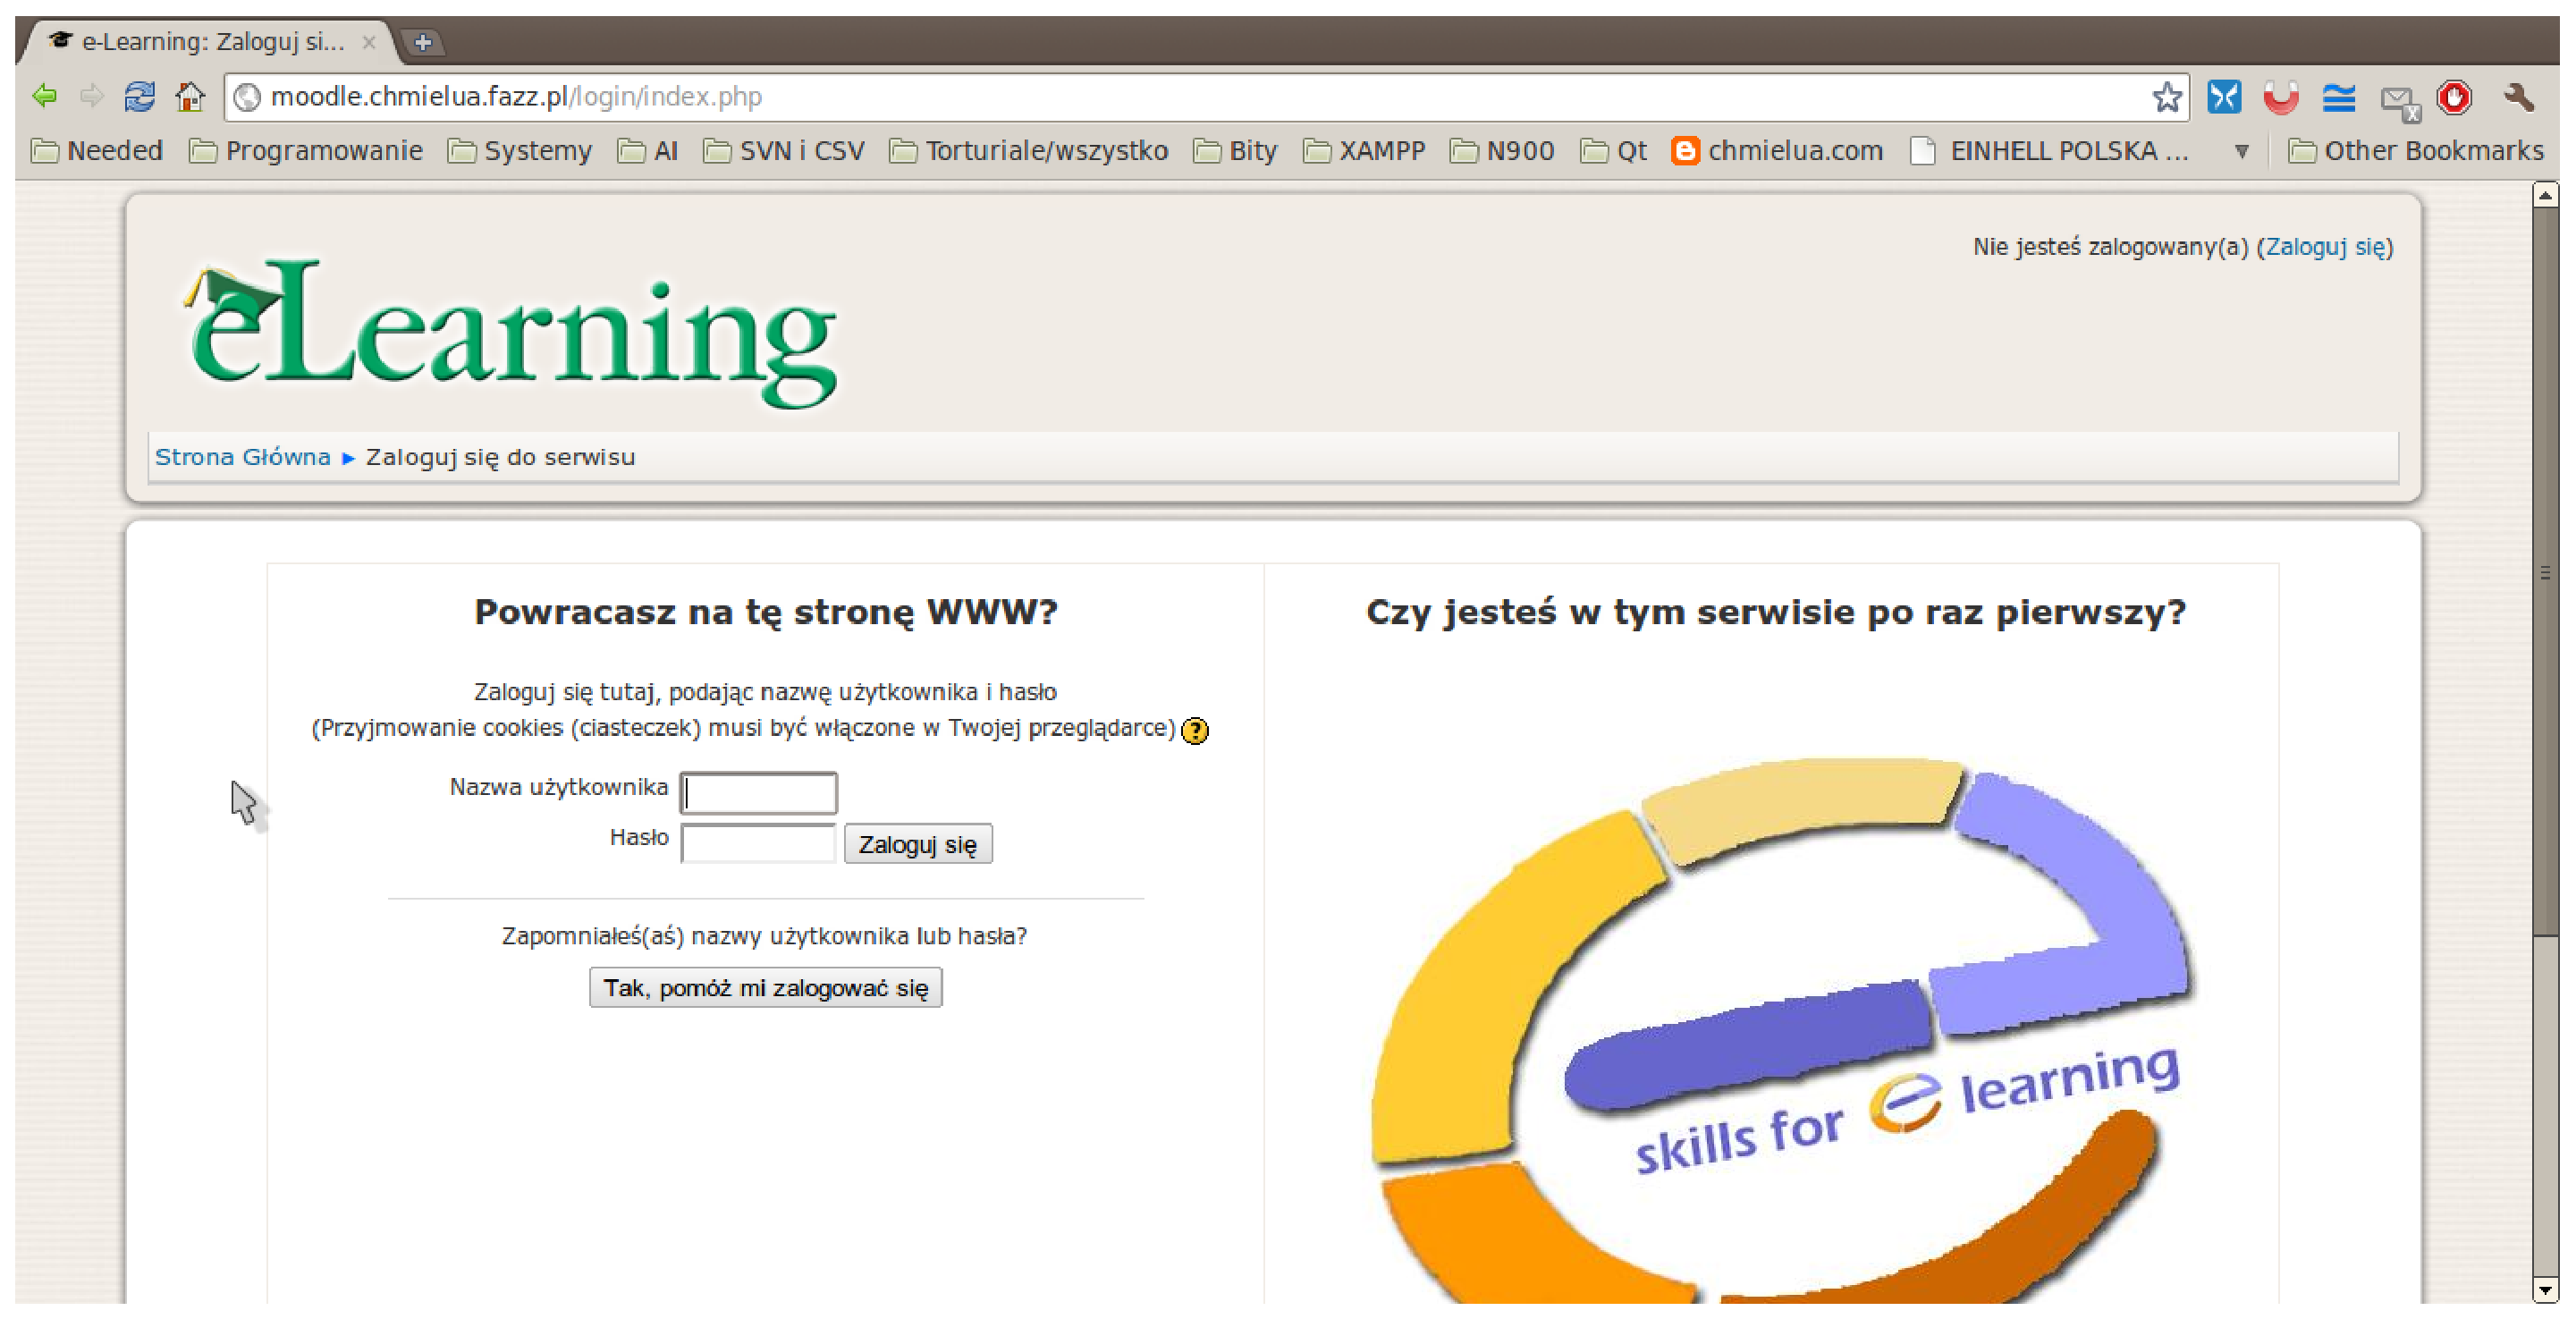
\includegraphics[width=1\textwidth]{projekt_sys//rys//logowanie.eps}
\end{figure}
Gdzie w przypadku braku konta, należy skorzystać z opcji \textit{Zacznij teraz od utworzenia nowego konta} rys. \ref{rys:nowy}.
\begin{figure}[!h]
	\centering
		\caption{Załorzenie nowego konta} \label{rys:nowy}
		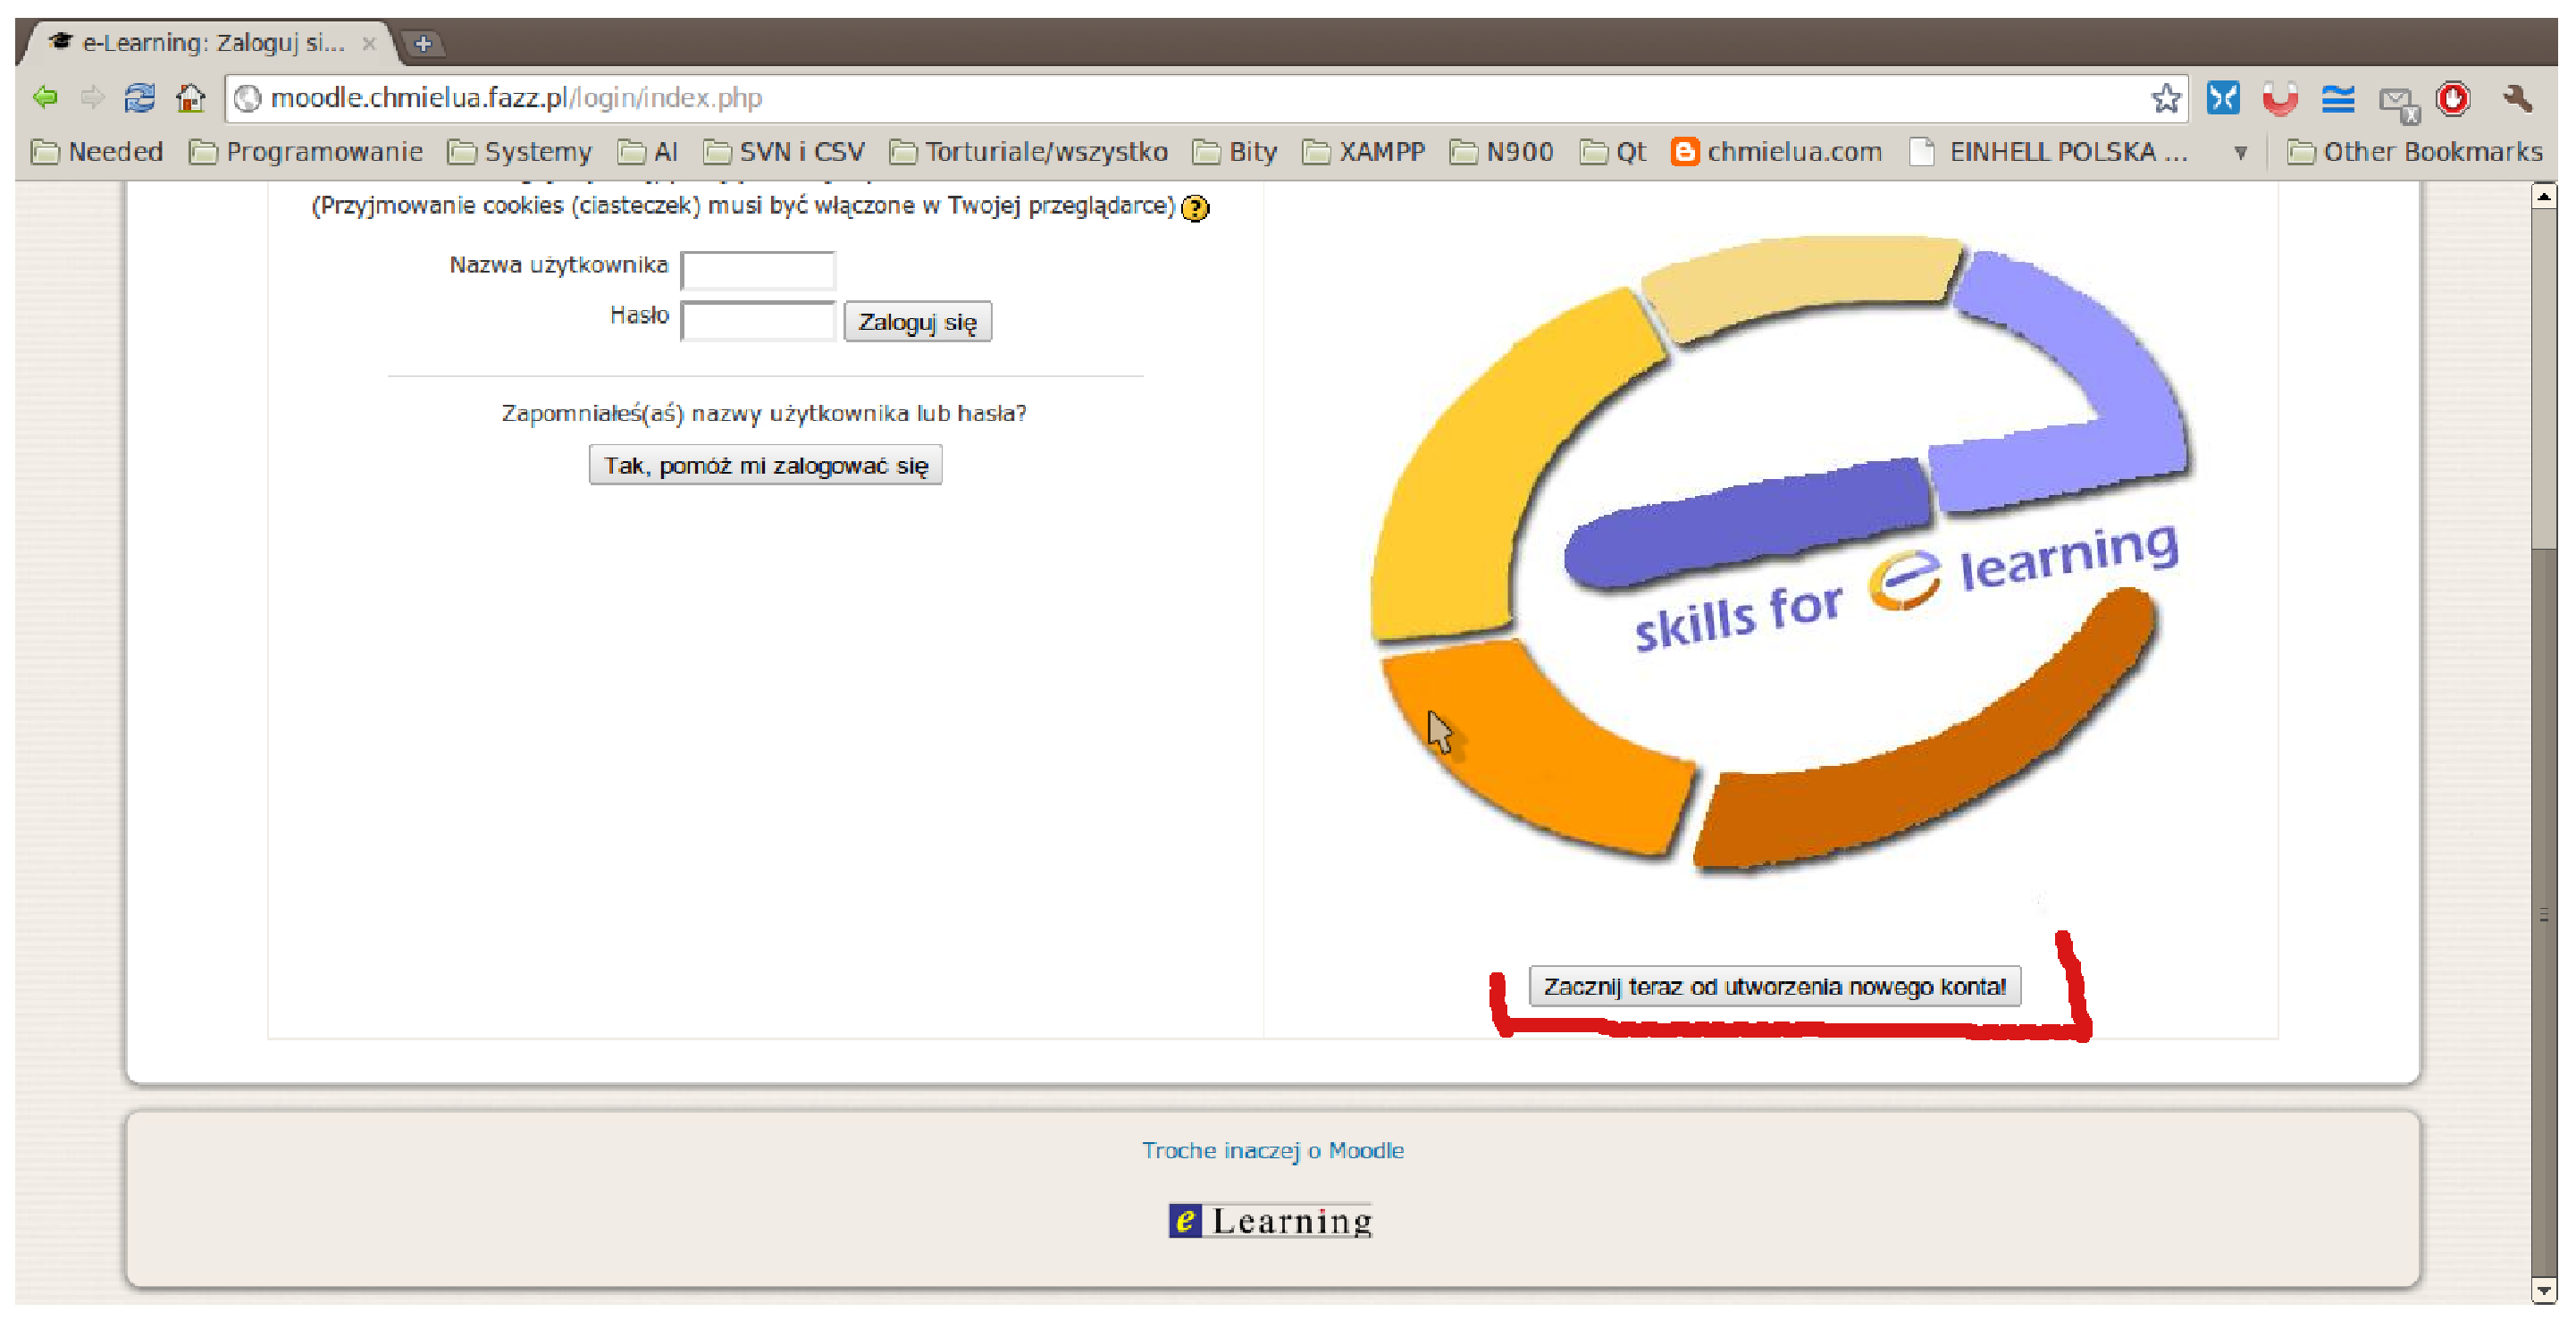
\includegraphics[width=1\textwidth]{projekt_sys//rys//nowy_user.eps}
\end{figure}
Po nacisnięciu \textit{Zacznij teraz od utworzenia nowego konta} zostaniemy przniesieni pod adres \href{http://moodle.chmielua.fazz.pl/login/signup.php?}{\textit{http://moodle.chmielua.fazz.pl/login/signup.php?}} rys.\ref{rys:signup}.
\begin{figure}[!h]
	\centering
		\caption{Formularz rejestracyjny} \label{rys:signup}
		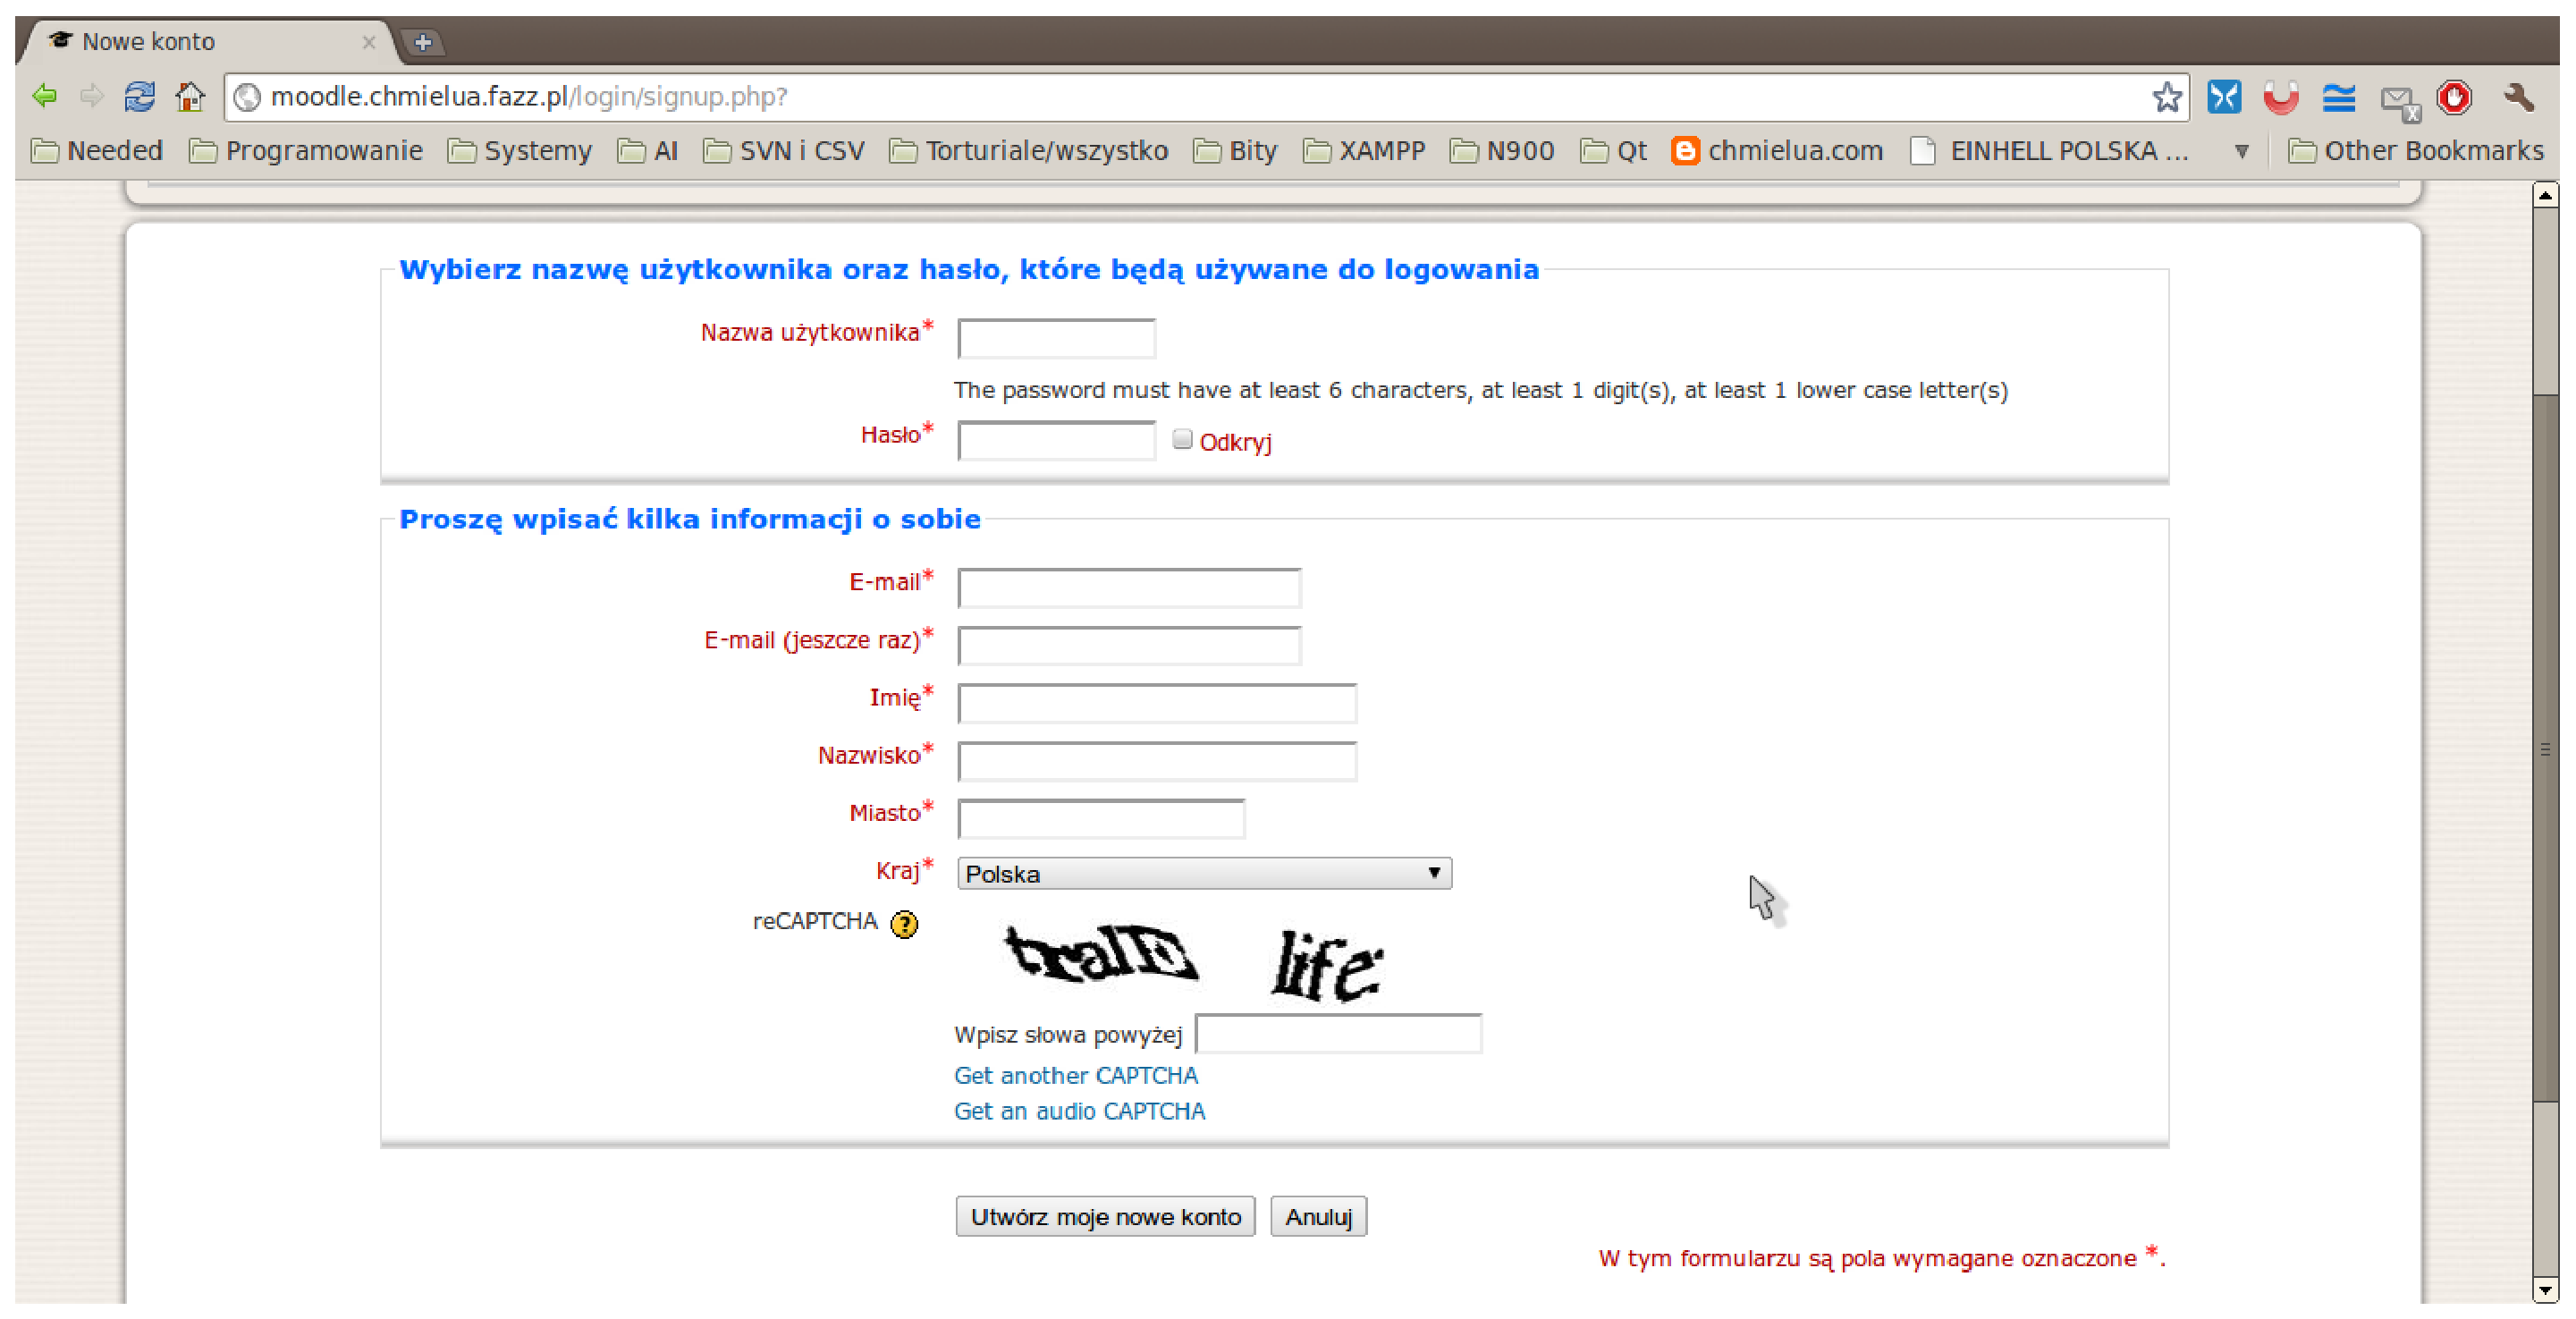
\includegraphics[width=1\textwidth]{projekt_sys//rys//rejestracja.eps}
\end{figure}
W celu wypełnienia formularza. Na jego podstawie zostanie utworzone nowe konto. Konto należy uwierzytelnić poprzez wejście w link wysłany w mailu na podany uprzednio adres. Dodawanie nowego użytkownika korzysta z zabezpieczenia reCAPTCHA, które chroni nas przed automatycznym tworzeniem nowych kont, które głównie są wykorzystywane do rozsyłania spamu. W przypadku gdy użytkownik zapomnie nazwę użytkownika lub hasło. Należy skorzystać z opcji \textit{Tak, pomóż mi zalogować się}. Po skorzystaniu z tej opcji zostajemy przeniesieni pod adres \href{http://moodle.chmielua.fazz.pl/login/forgot_password.php}{\textit{http://moodle.chmielua.fazz.pl/login/forgot\_password.php}} rys.\ref{rys:lost_pass}
\begin{figure}[!h]
	\centering
		\caption{Zapomniane hasło} \label{rys:lost_pass}
		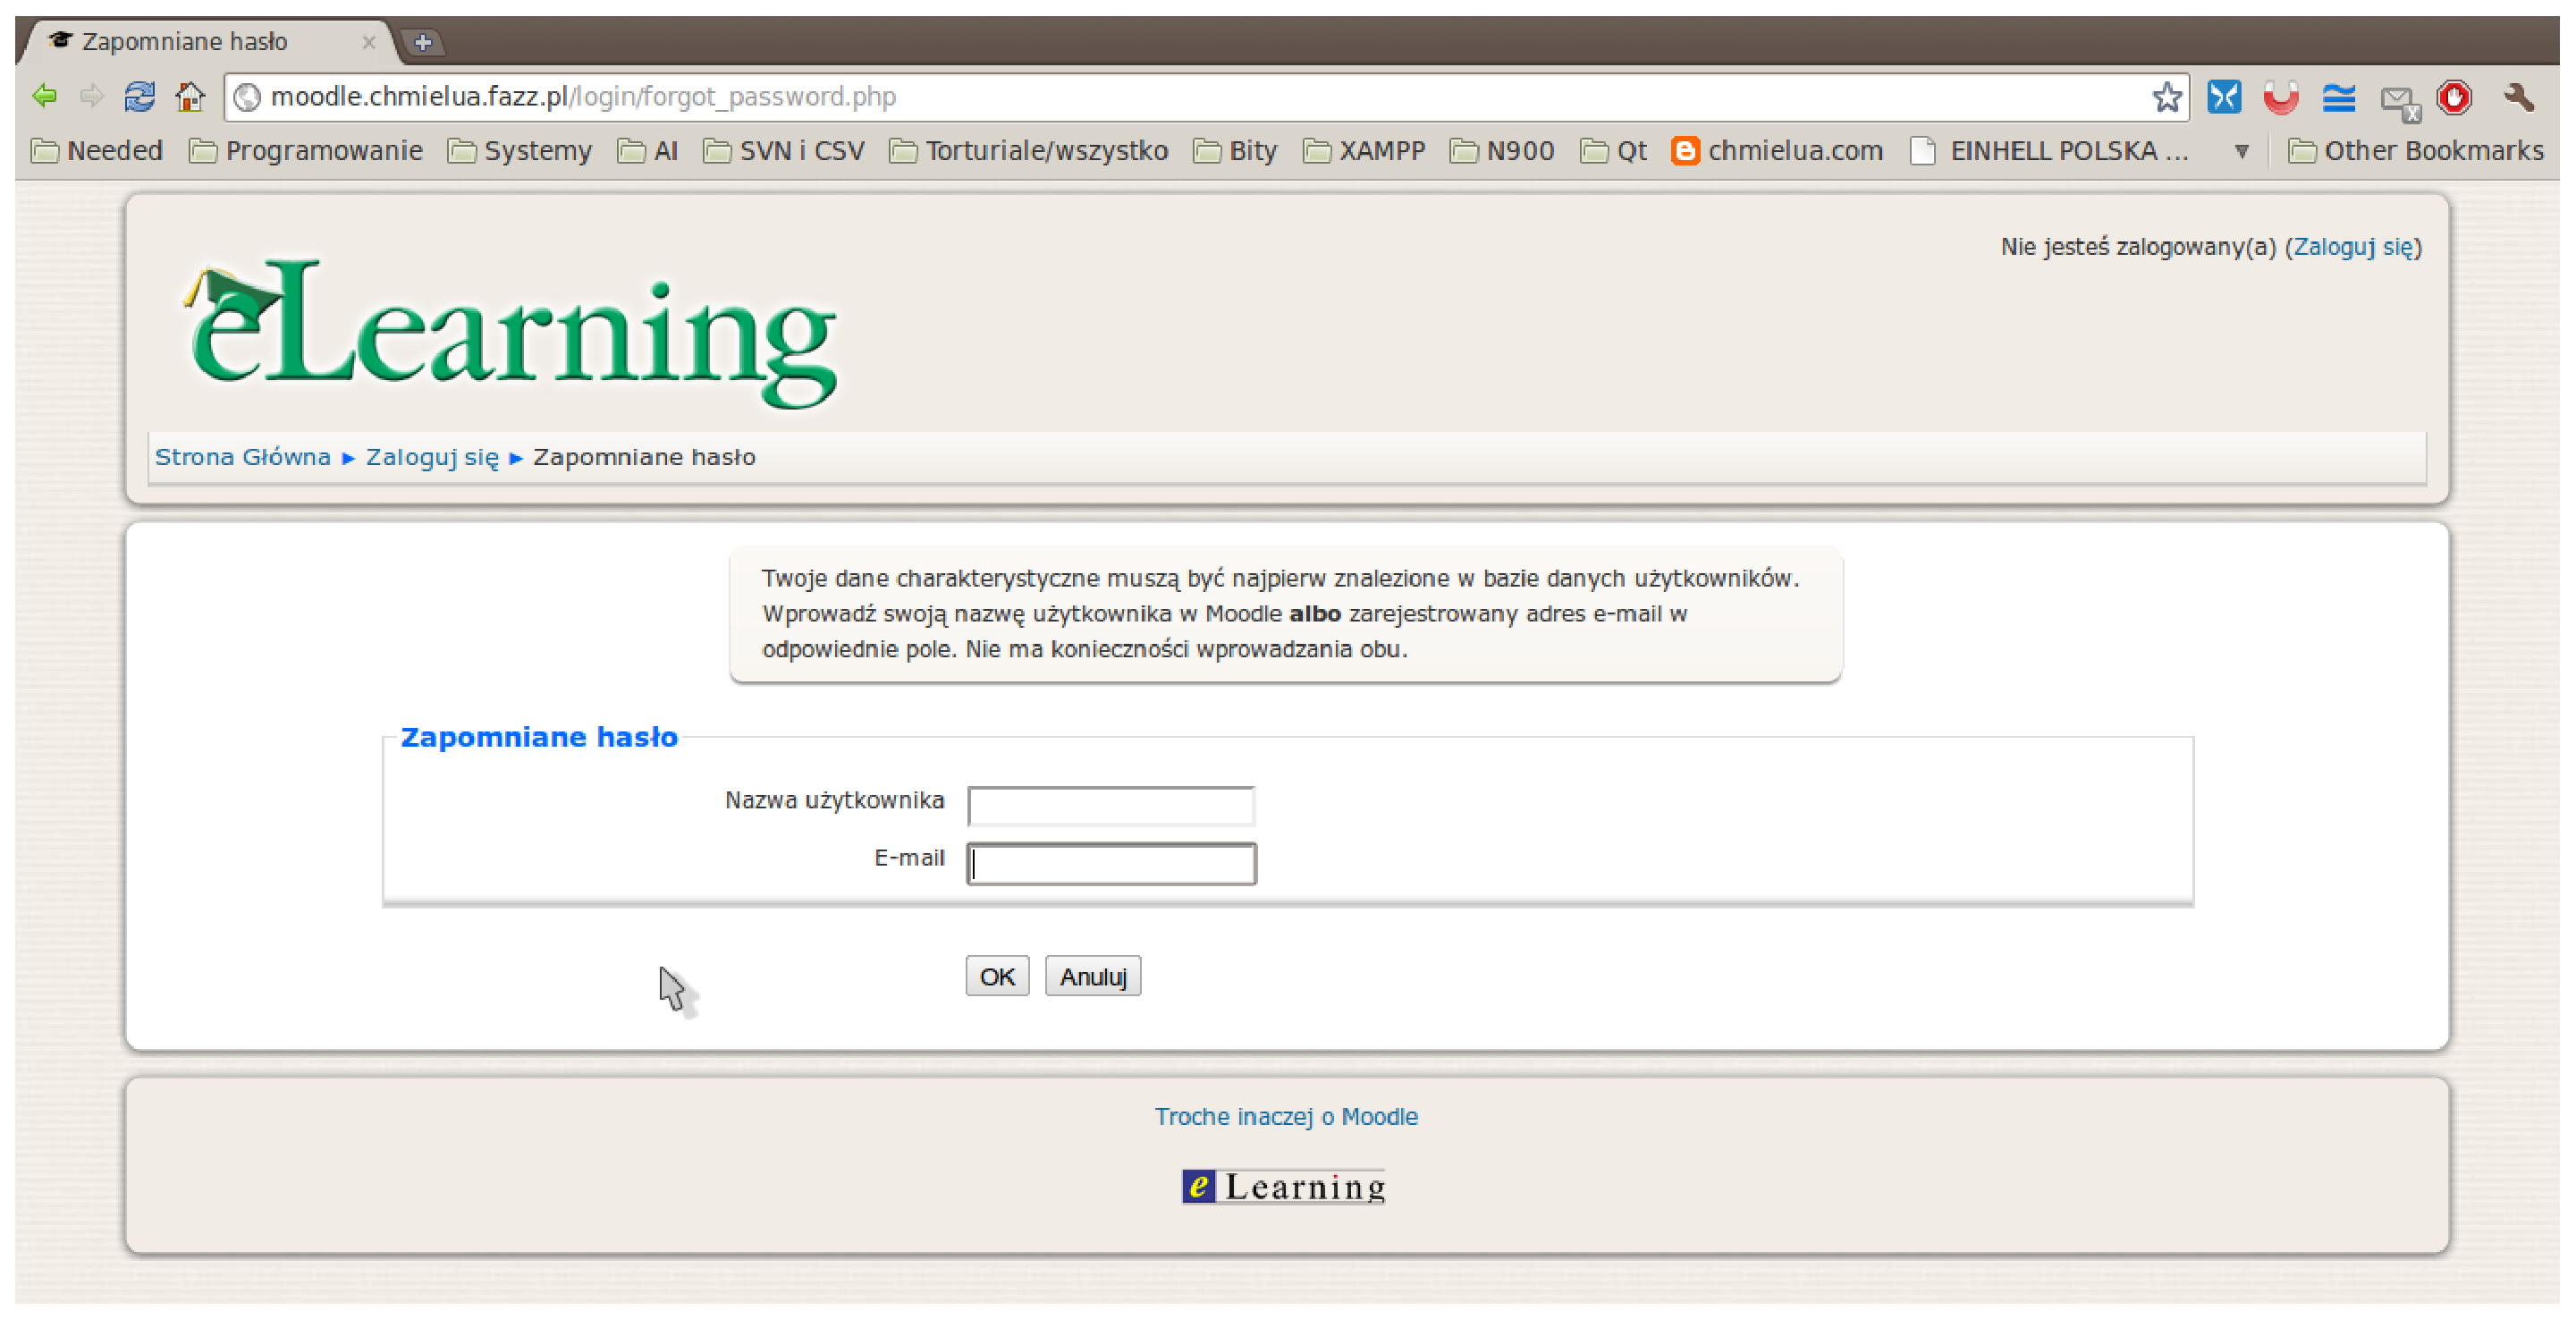
\includegraphics[width=1\textwidth]{projekt_sys//rys//lost_pass.eps}
\end{figure}
Na stronie należy wypełnić jedno z dwóch pól i wcisnąć \textit{OK}. Zostanie wysłana wiadomość, gdzie aby potwierdzić i otrzymać nowe hasło za pośrednictwem poczty elektronicznej, nalezy przejść na podana pod spodem stronę. Strona ta powinna wyglądać tak jak na rys.\ref{rys:new_pass}.
\begin{figure}[!h]
	\centering
		\caption{Automatyczna generacja nowego hasła} \label{rys:new_pass}
		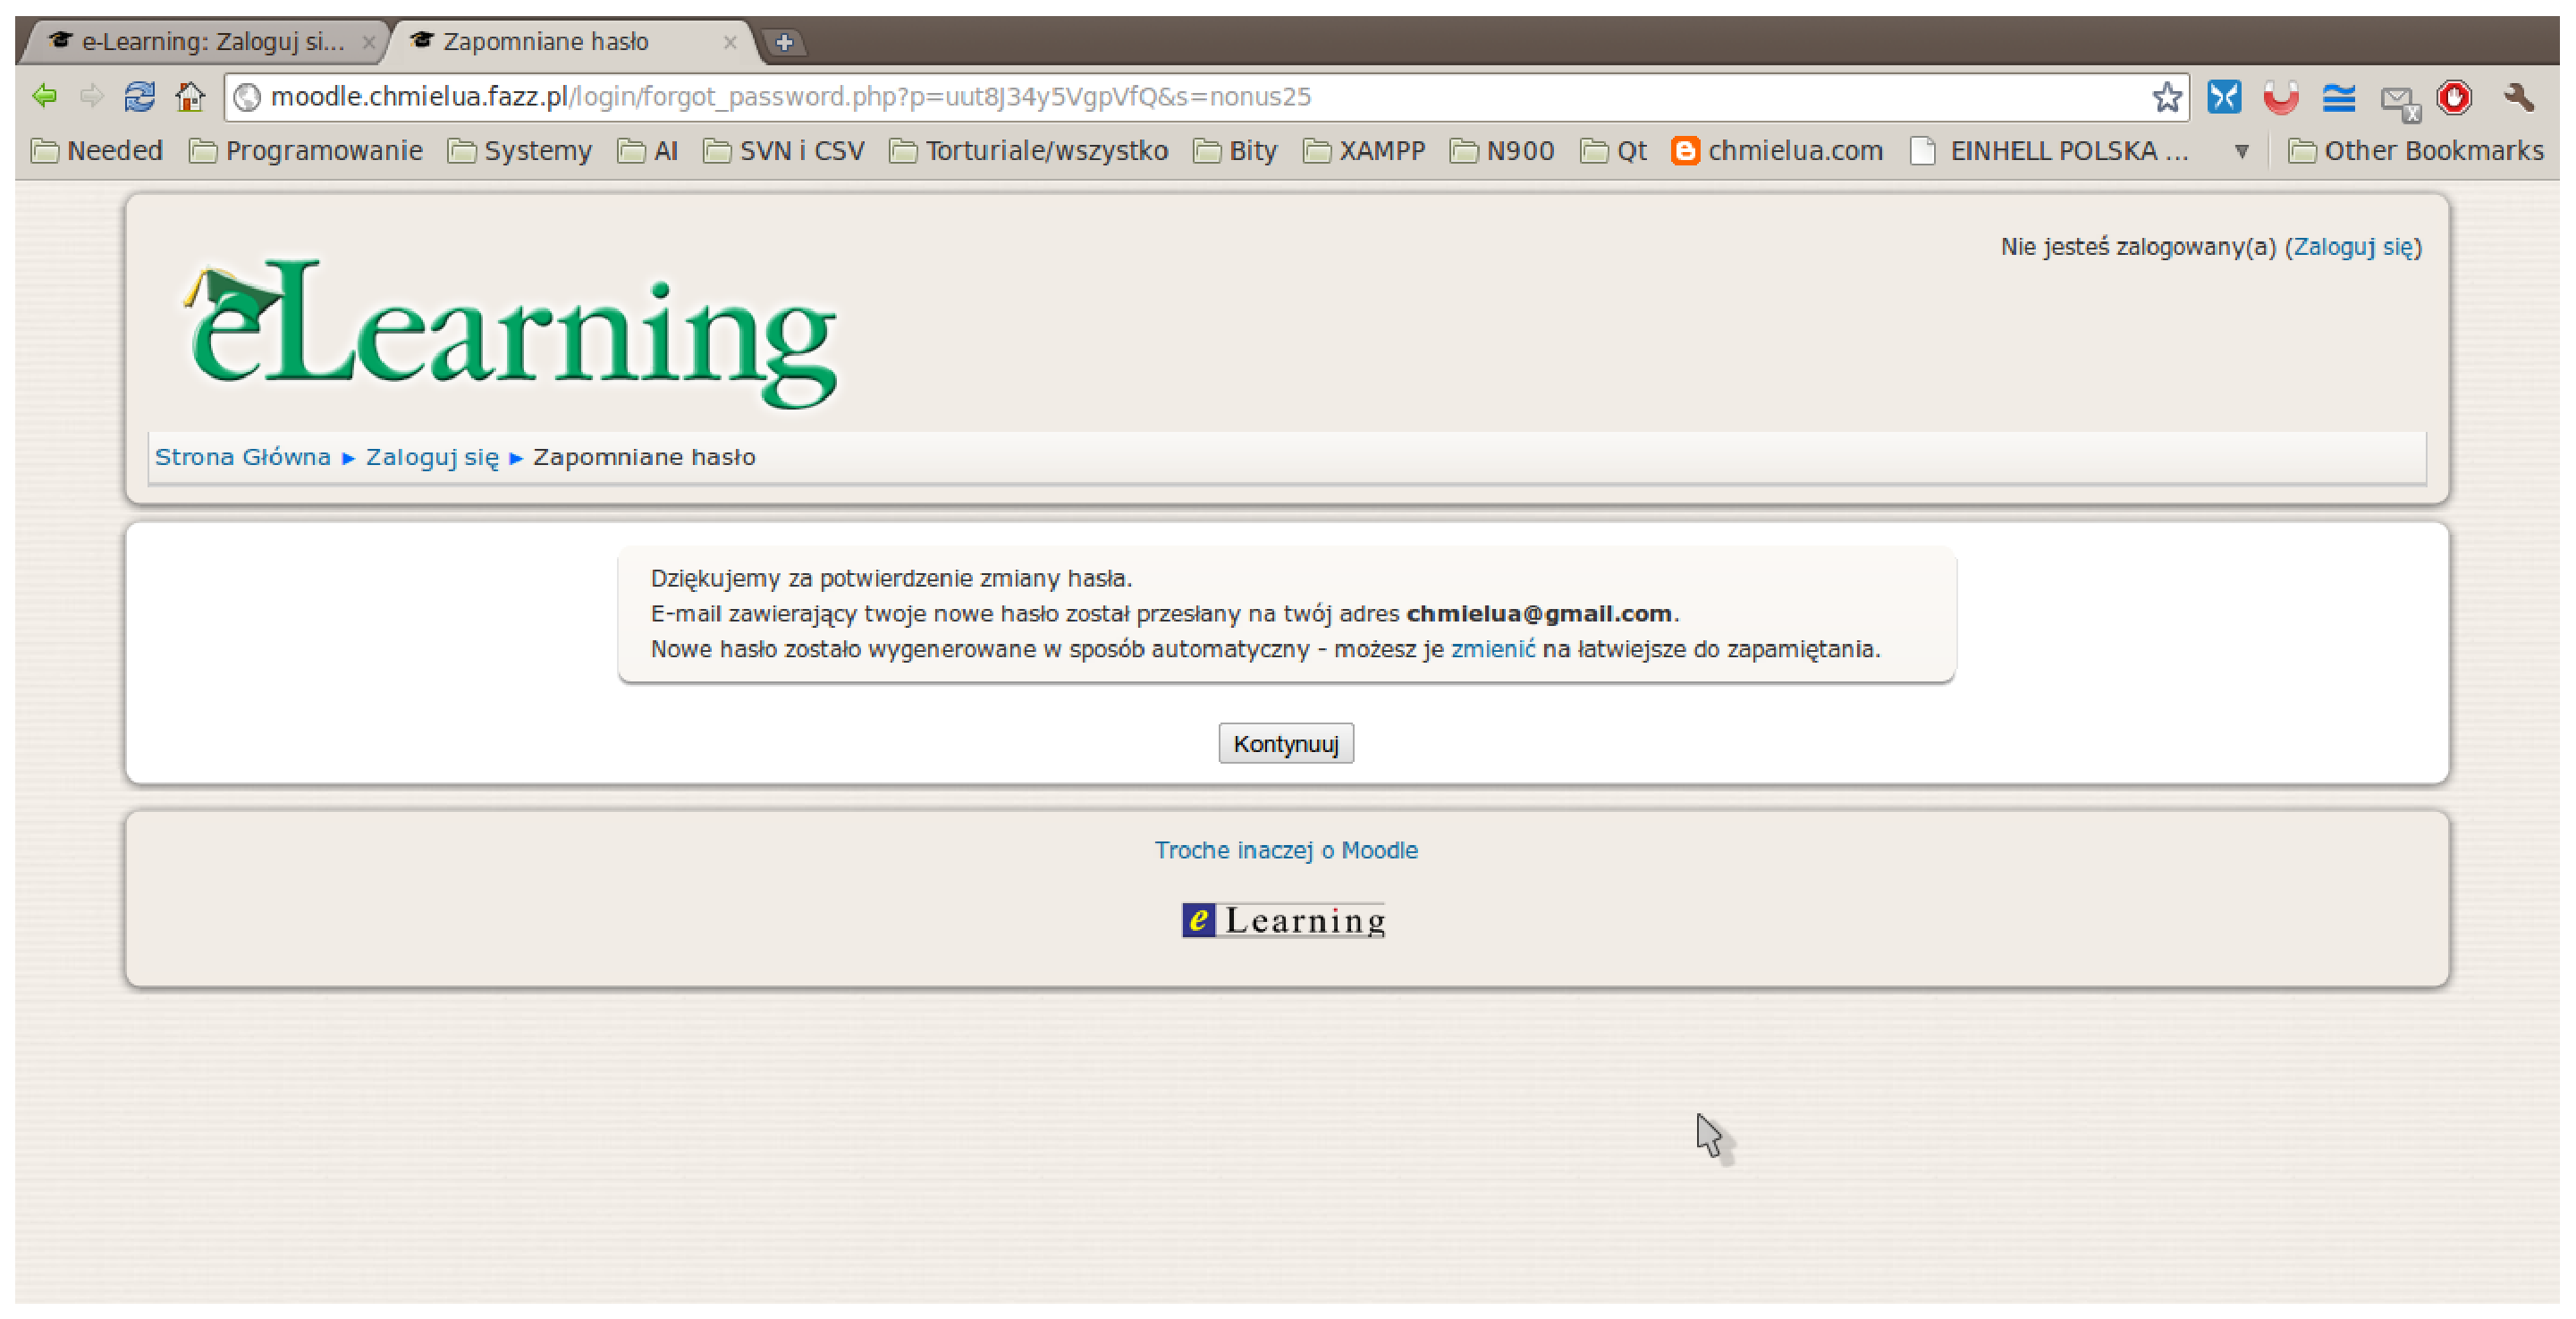
\includegraphics[width=1\textwidth]{projekt_sys//rys//nowe_haslo.eps}
\end{figure}
Po wciśnięciu kontynuuj zostanie ponownie wyslana wiadomość do nas. Wiadomość ta będzie zawierać nowe hasło, nazwę użytkownika i link do zmiany wygenerowanego hasła. Gdy przejdziemy do strony odpowiedającej za zmiane hasła\ref{rys:zmien_haslo} należy podać hasło, które zostało do nas wysłane, a następnie podać swoje własne nowe hasło. 
\begin{figure}[!h]
	\centering
		\caption{Ręczna zmiana hasła} \label{rys:zmien_haslo}
		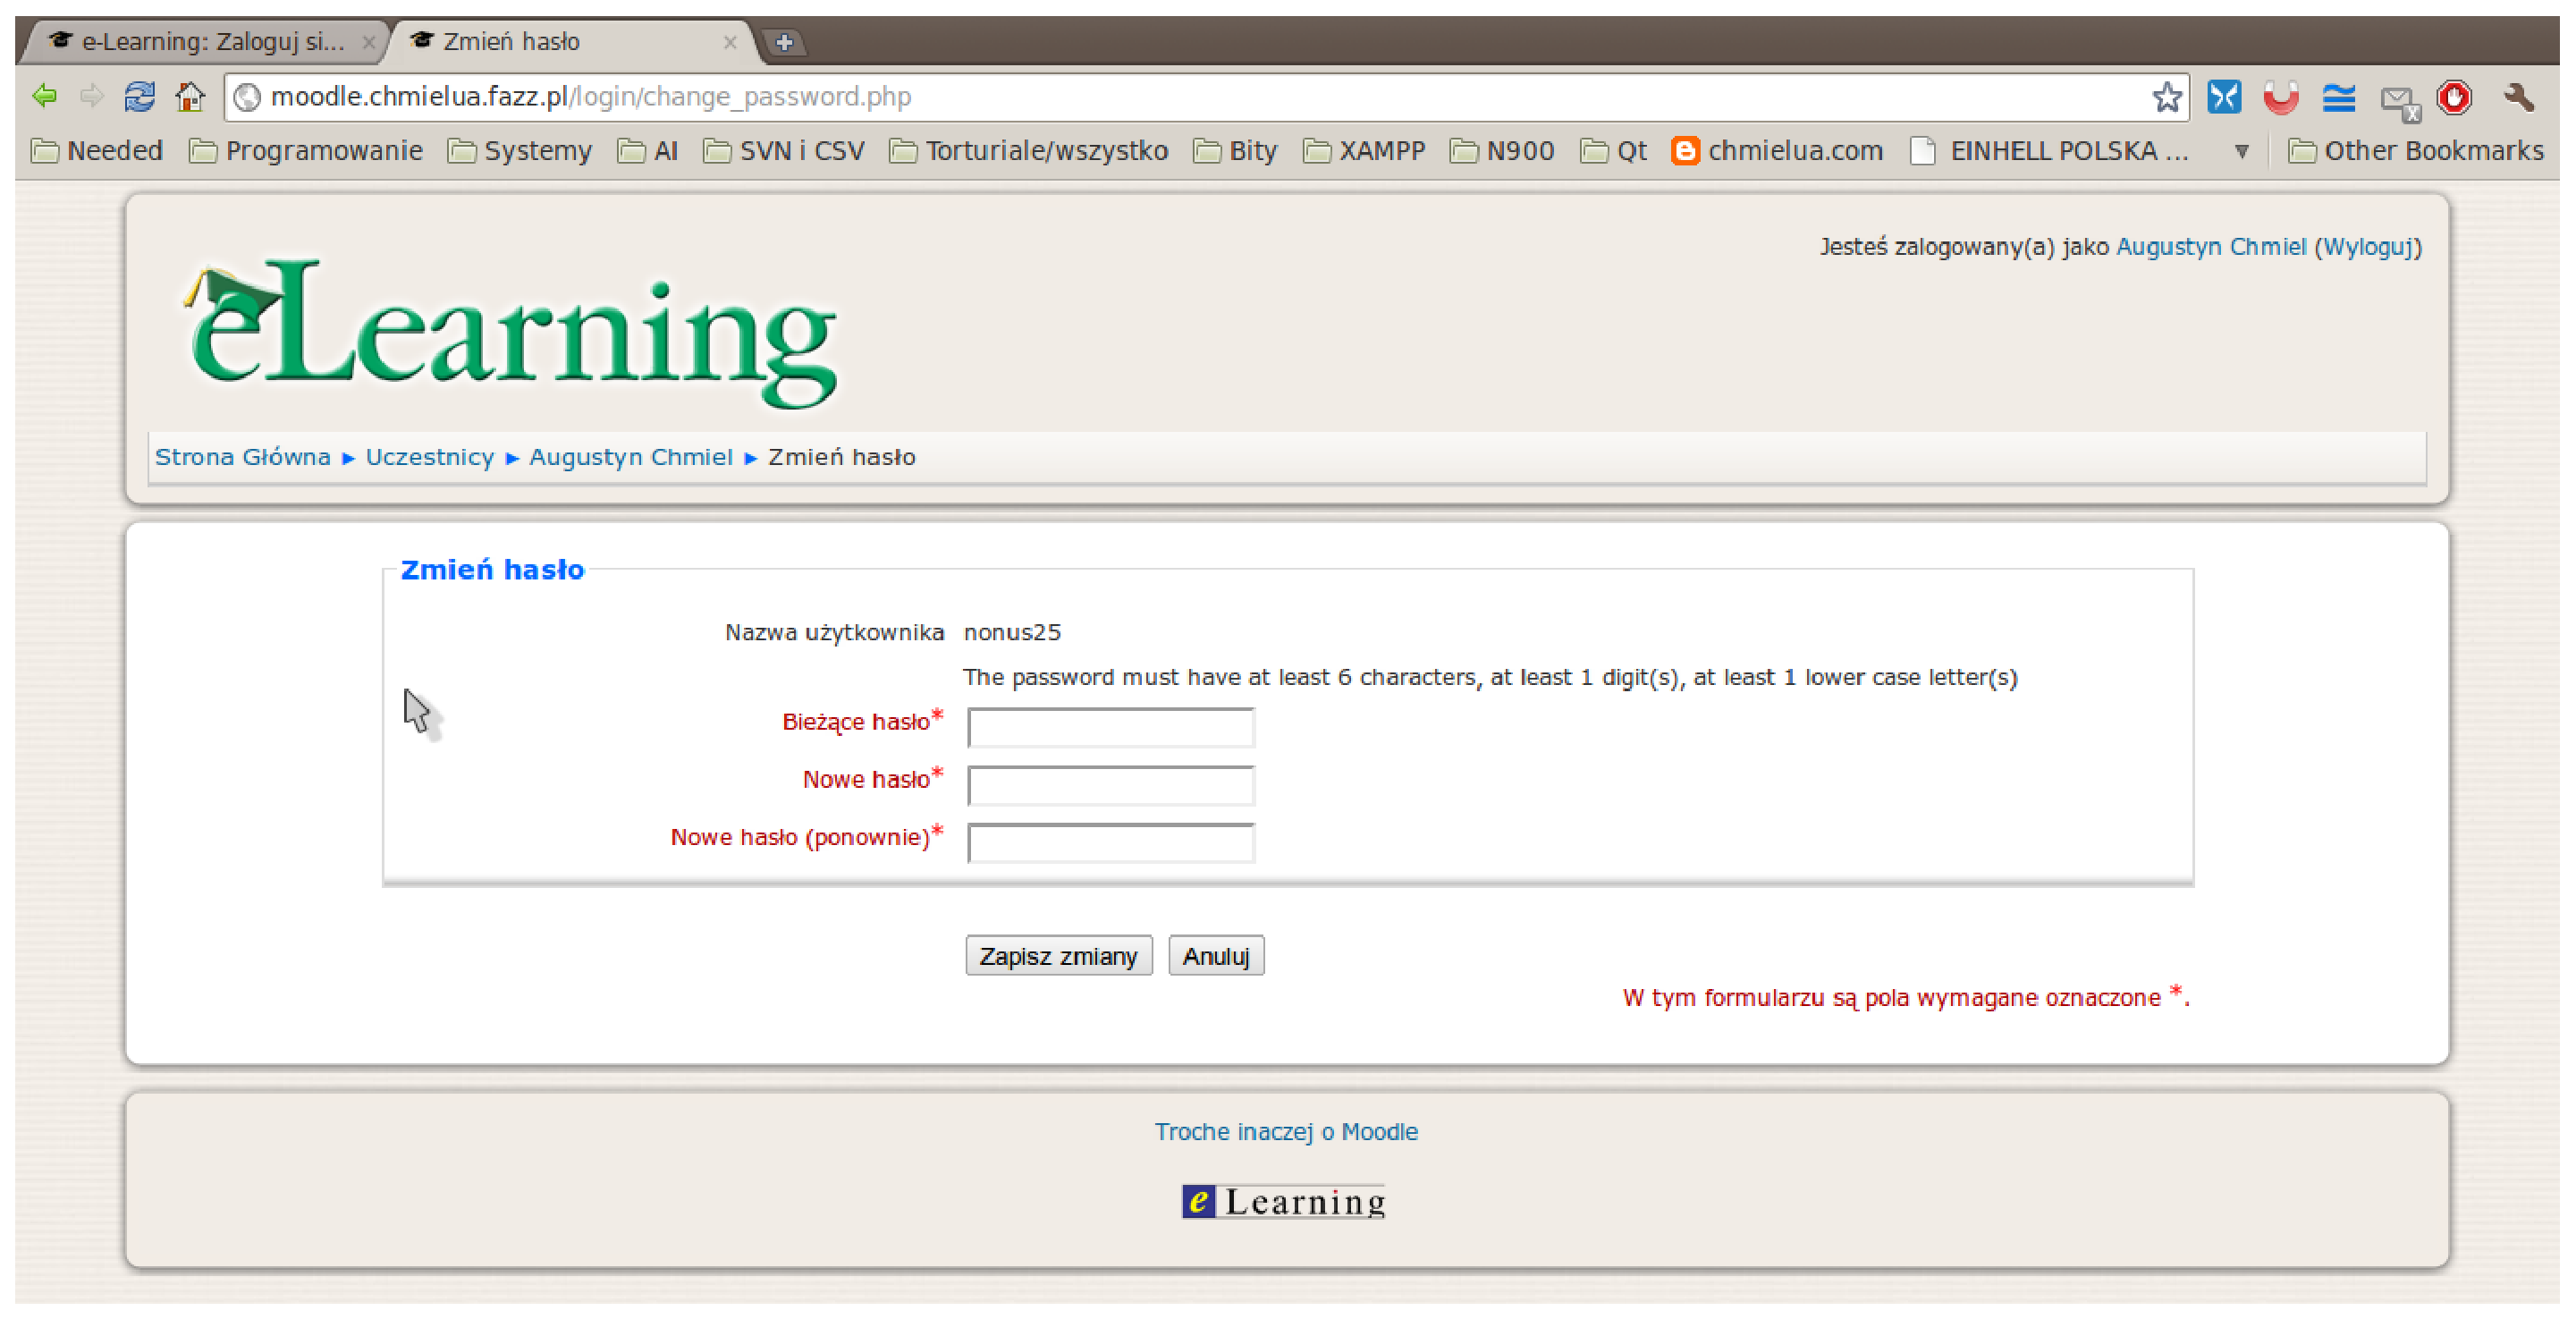
\includegraphics[width=1\textwidth]{projekt_sys//rys//zmiana_hasla.eps}
\end{figure}
Przy istniejącym kącie i po udanej próbie logowania jesteśmy wstanie zobaczyć strone główną witryny \href{http://moodle.chmielua.fazz.pl/}{\textit{http://moodle.chmielua.fazz.pl/}} rys. \ref{rys:glowna}
\begin{figure}[!h]
	\centering
		\caption{Strona główna} \label{rys:glowna}
		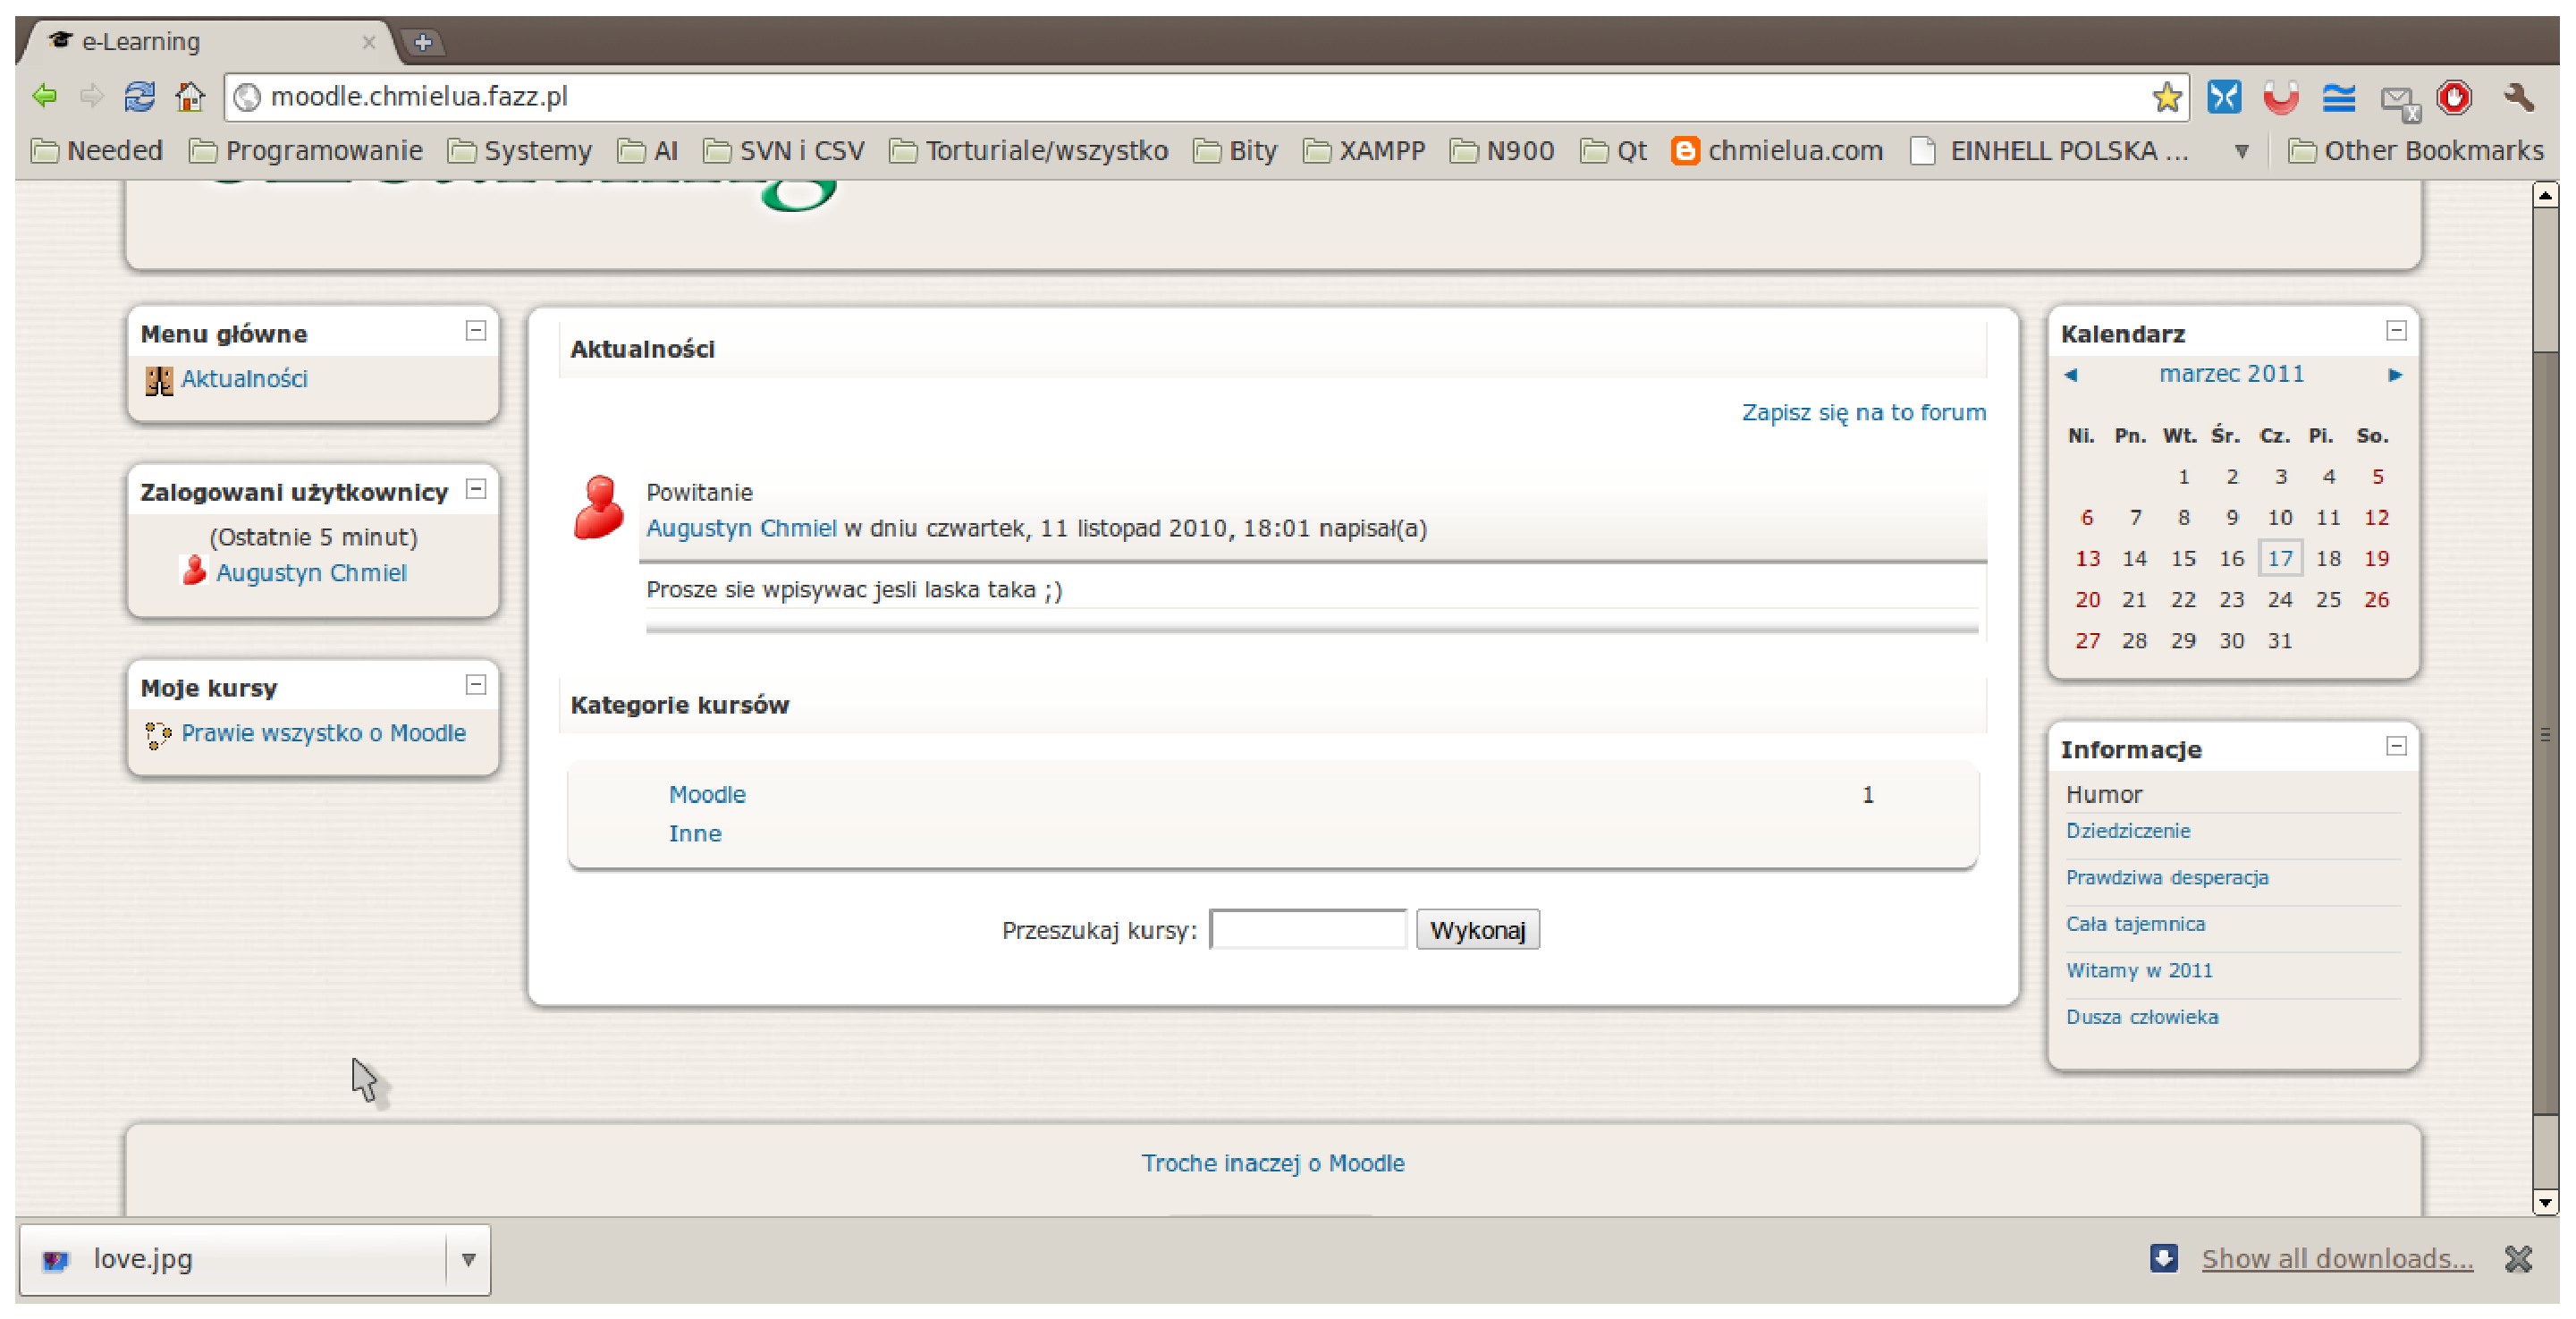
\includegraphics[width=1\textwidth]{projekt_sys//rys//glowna.eps}
\end{figure}
Na stronie głównej znajdują się podstawowe informacje takie jak Aktualności, Uczestnicy, Zalogowani użytkownicy, Kategorie kursów, Kalendarz i Humor zaciągnięty ze strony \href{http://demotywatory.pl/}{\textit{http://demotywatory.pl/}} przy wykorzystaniu kanału RSS\footnote{RSS – umowna rodzina języków znacznikowych do przesyłania nagłówków wiadomości i nowości na wybranych przez użytkownika RSS stronach.}. Następnie w bloku o tytule \textit{Kategorie kursów} znajdują się dwie kategorie \textit{Moodle} i \textit{Inne} co widać dokladnie na rys. \ref{rys:glowna}. Kategoria Moodle zawiera kurs który nosi nazwę \textit{Prawie wszystko o Moodle} rys. \ref{rys:kurs}
\begin{figure}[!h]
	\centering
		\caption{Kategorja Moodle} \label{rys:kurs}
		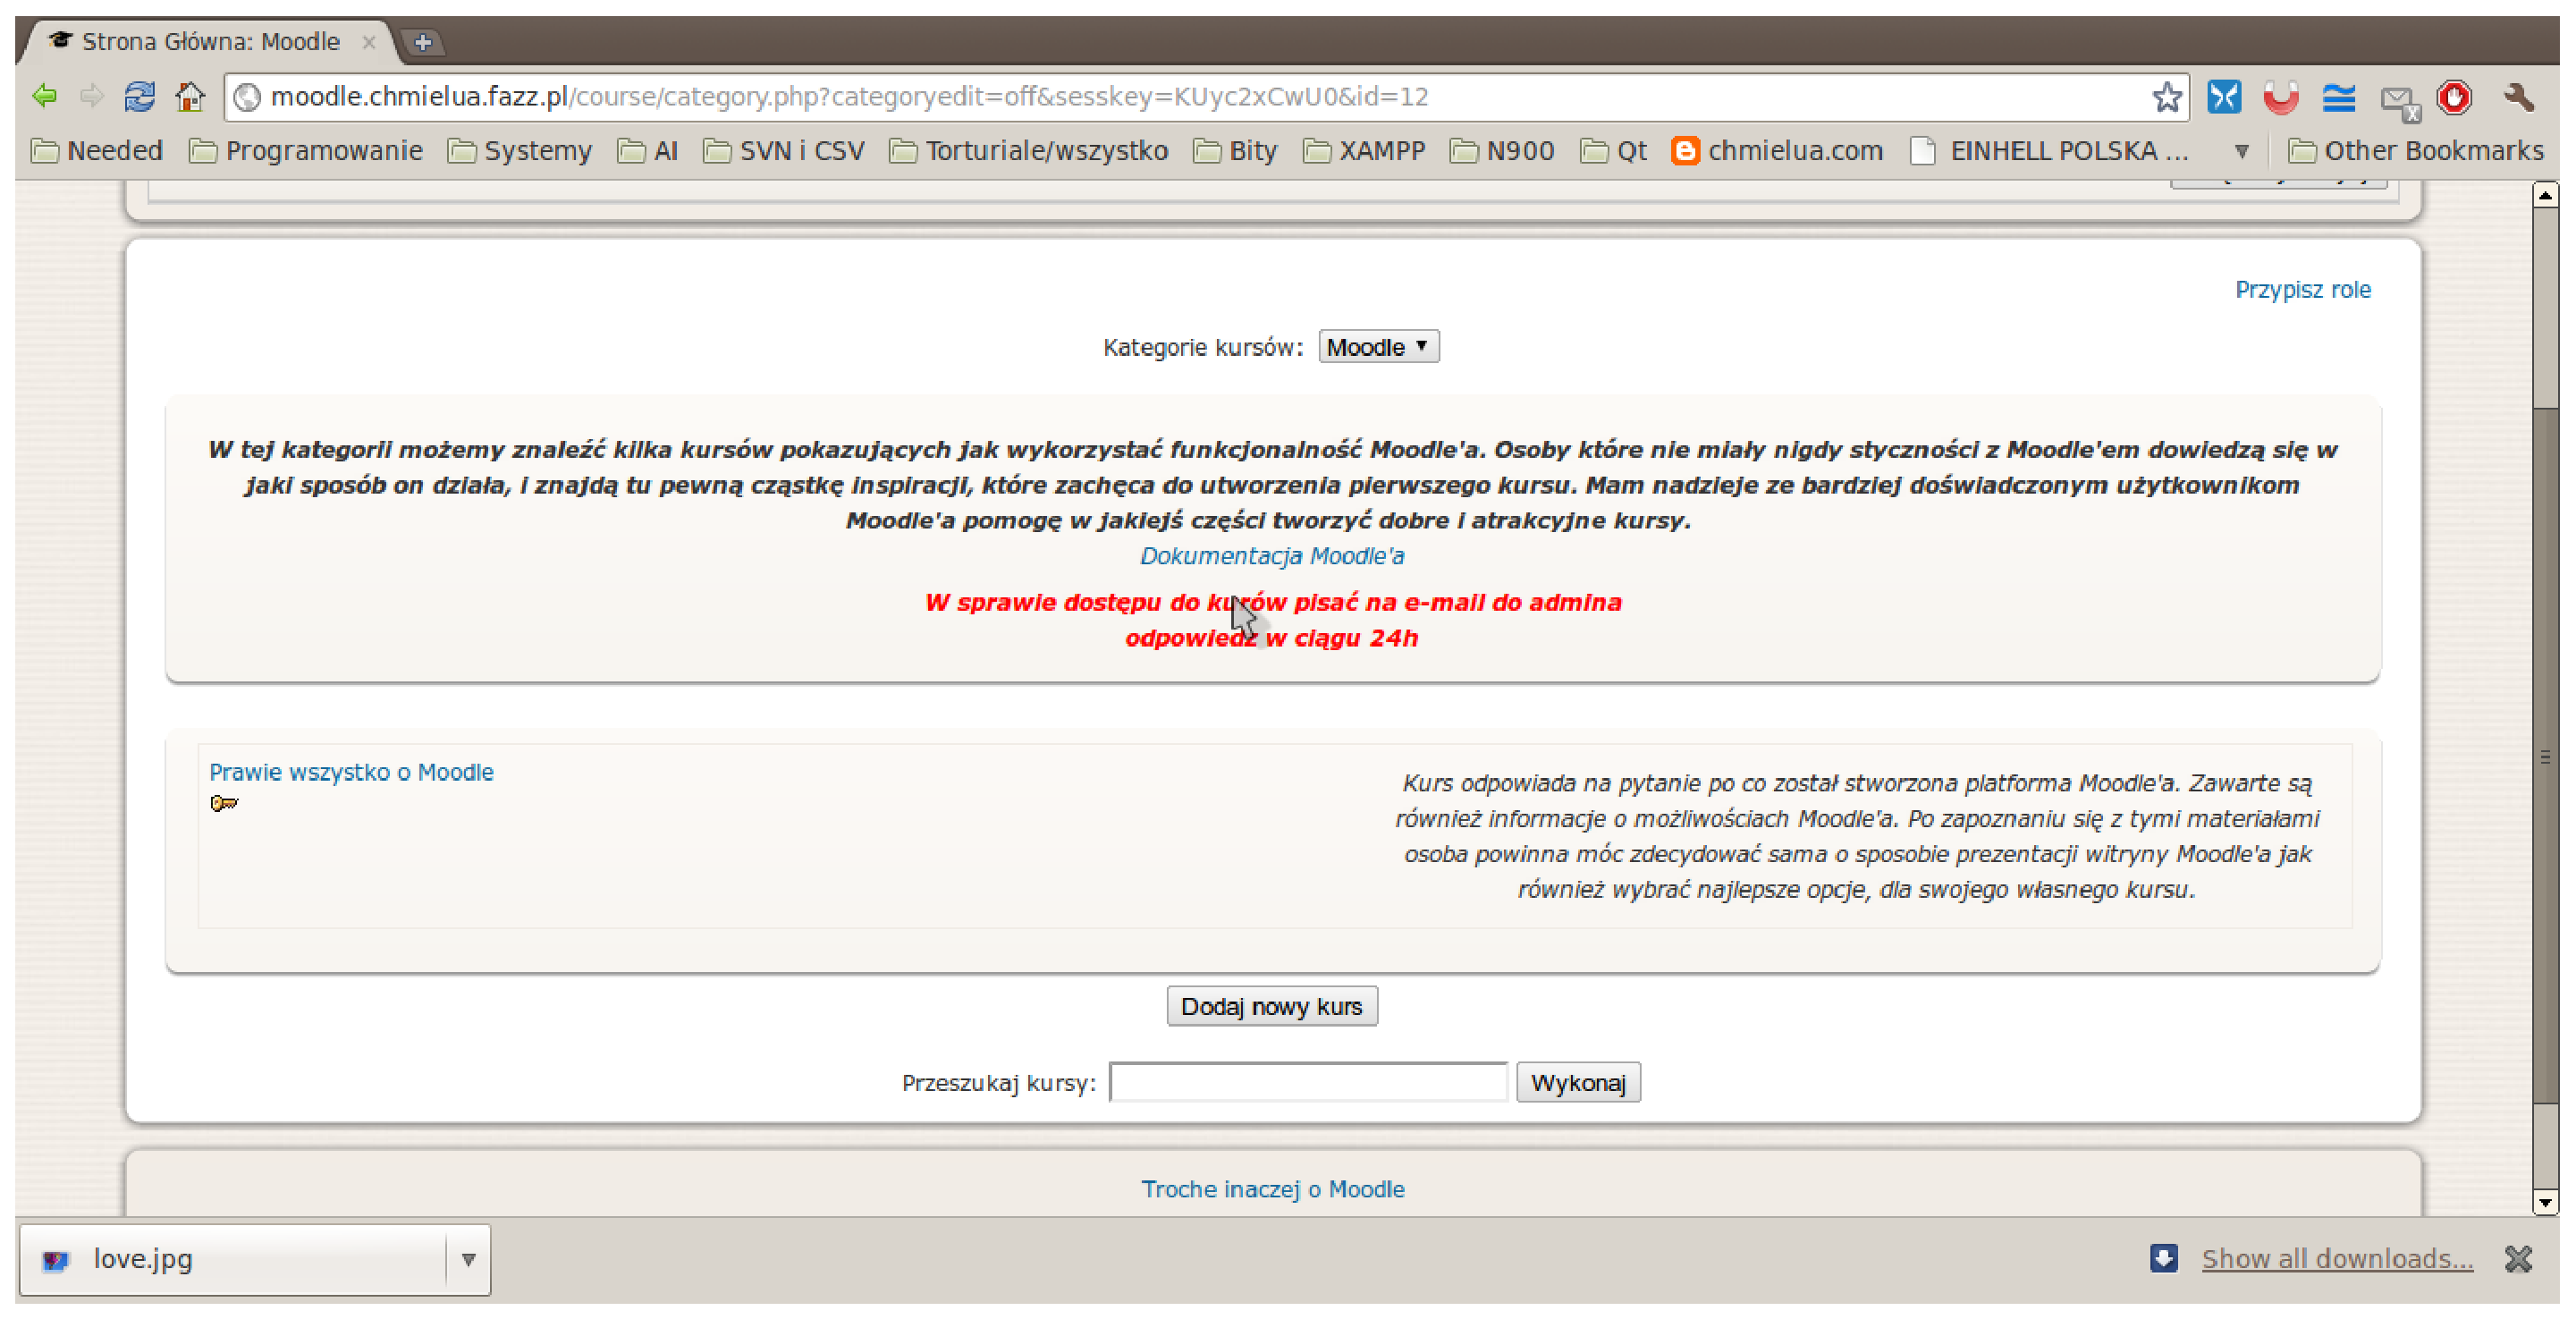
\includegraphics[width=1\textwidth]{projekt_sys//rys//kurs.eps}
\end{figure}
\begin{figure}[!h]
	\centering
		\caption{Kurs: Prawie wszystko o Moodle} \label{rys:kurs_moodle}
		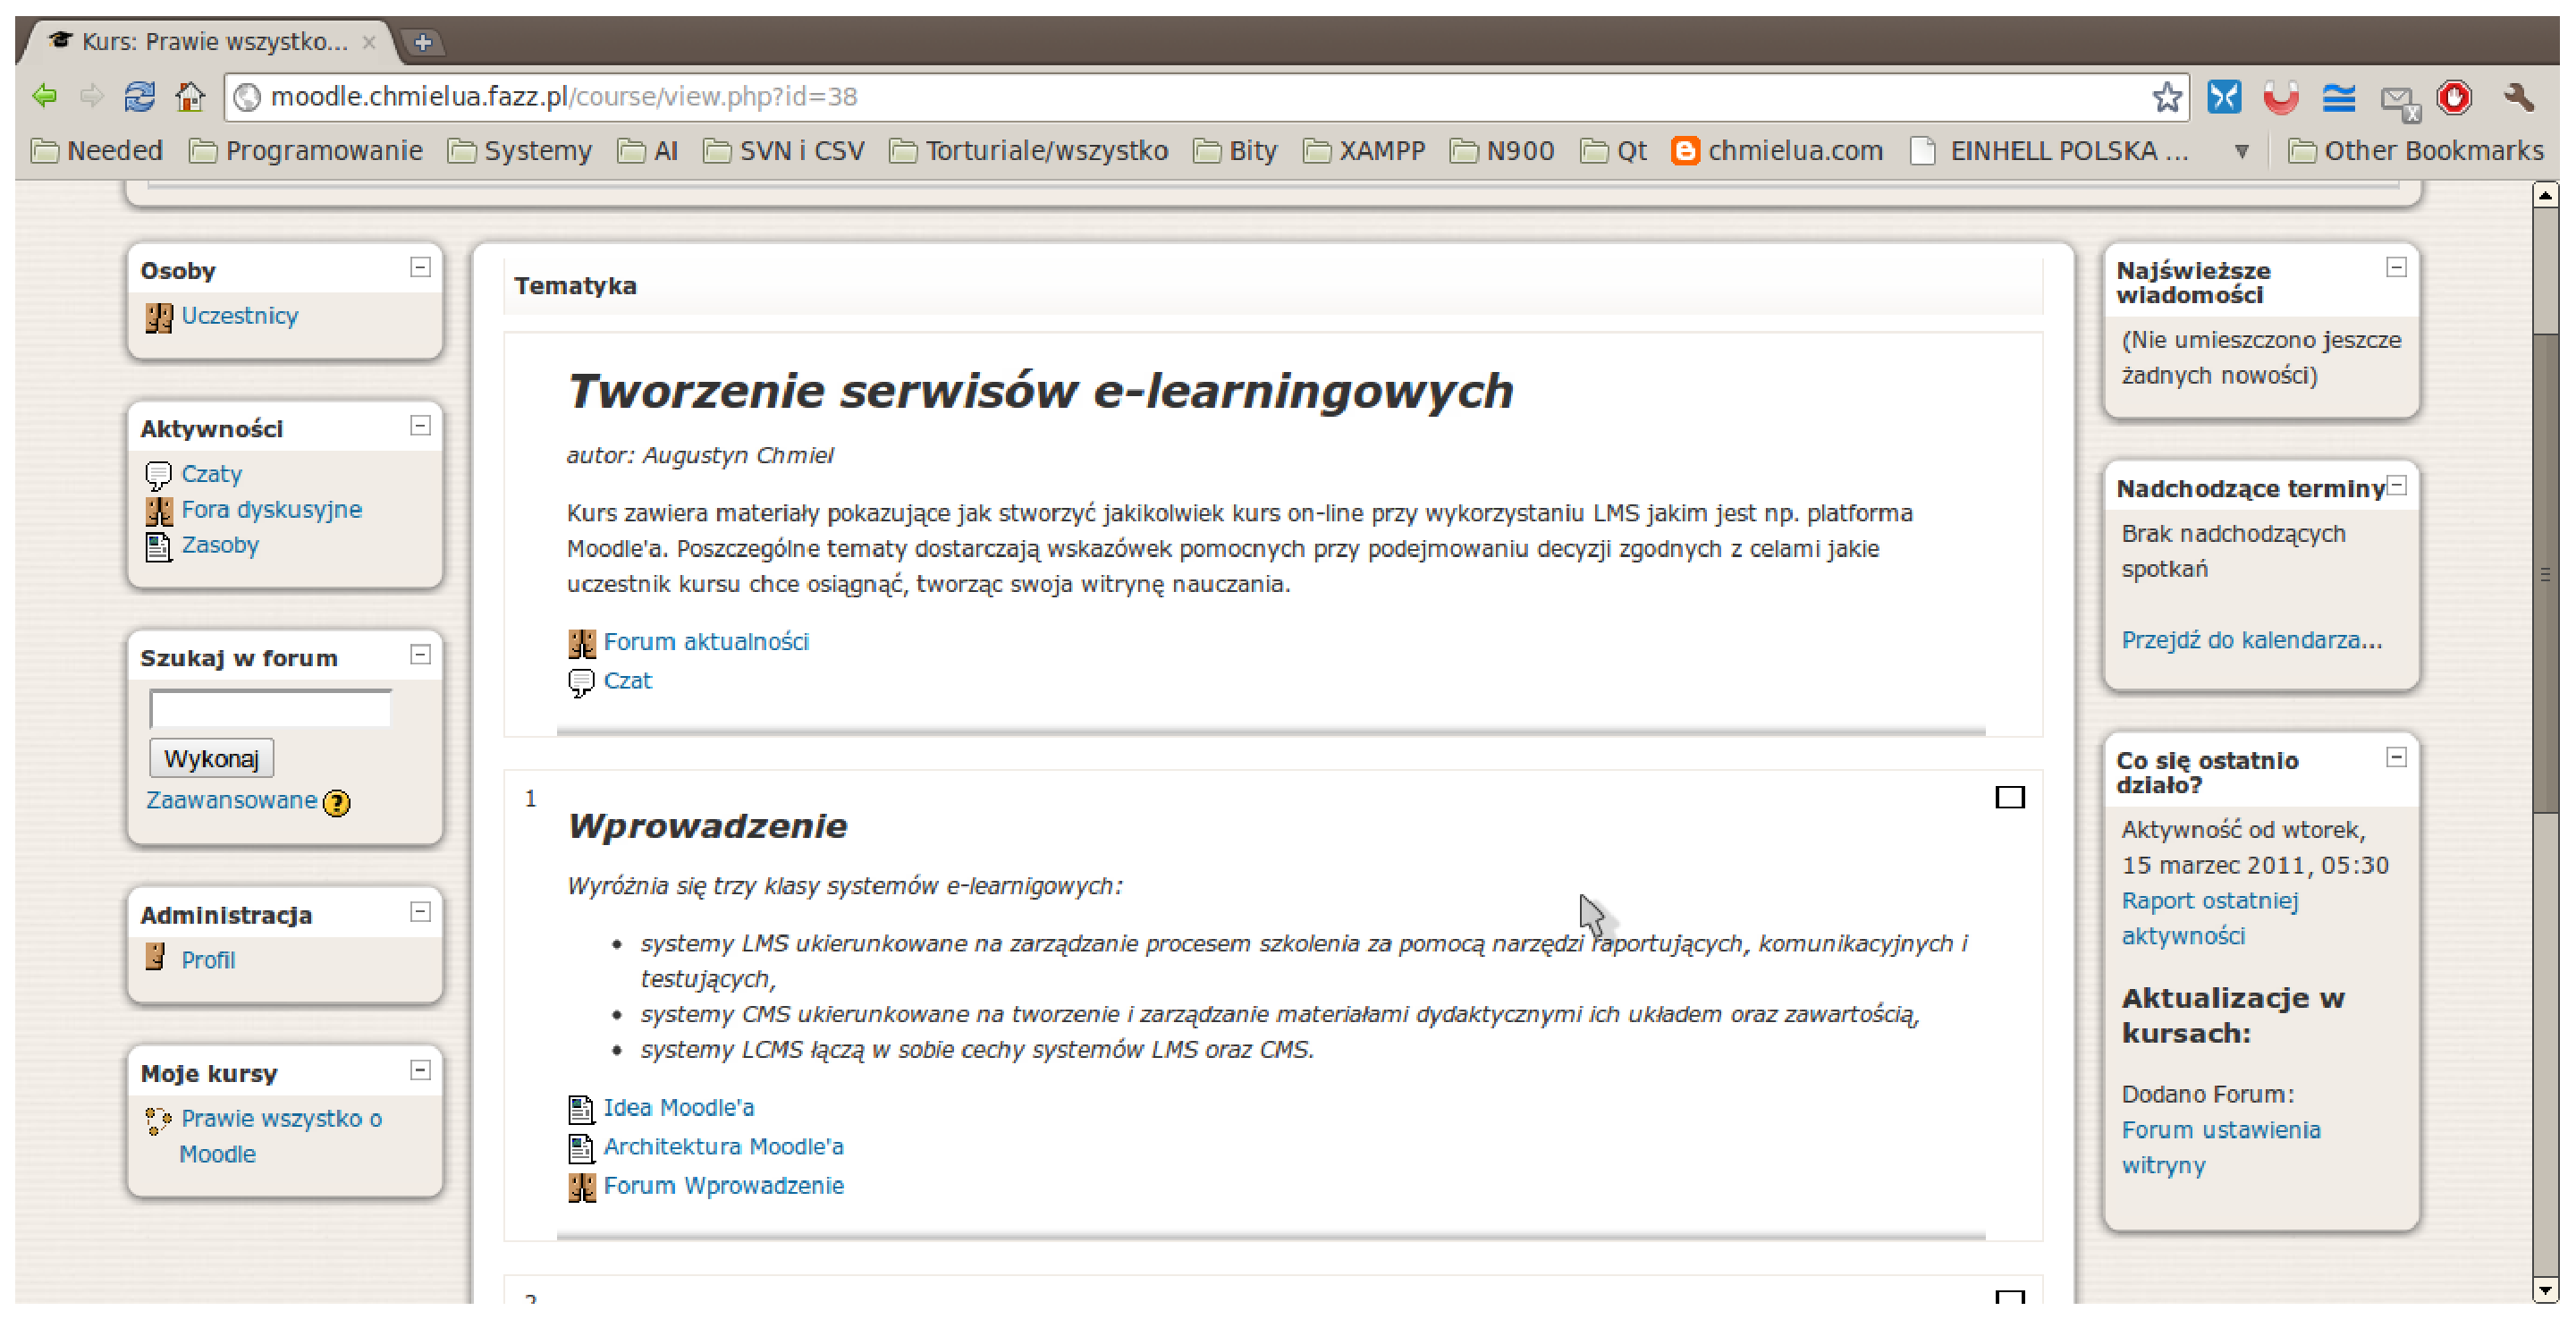
\includegraphics[width=1\textwidth]{projekt_sys//rys//kurs_moodle.eps}
\end{figure}
\begin{figure}[!h]
	\centering
		\caption{Kurs: Prawie wszystko o Moodle} \label{rys:kurs_moodle2}
		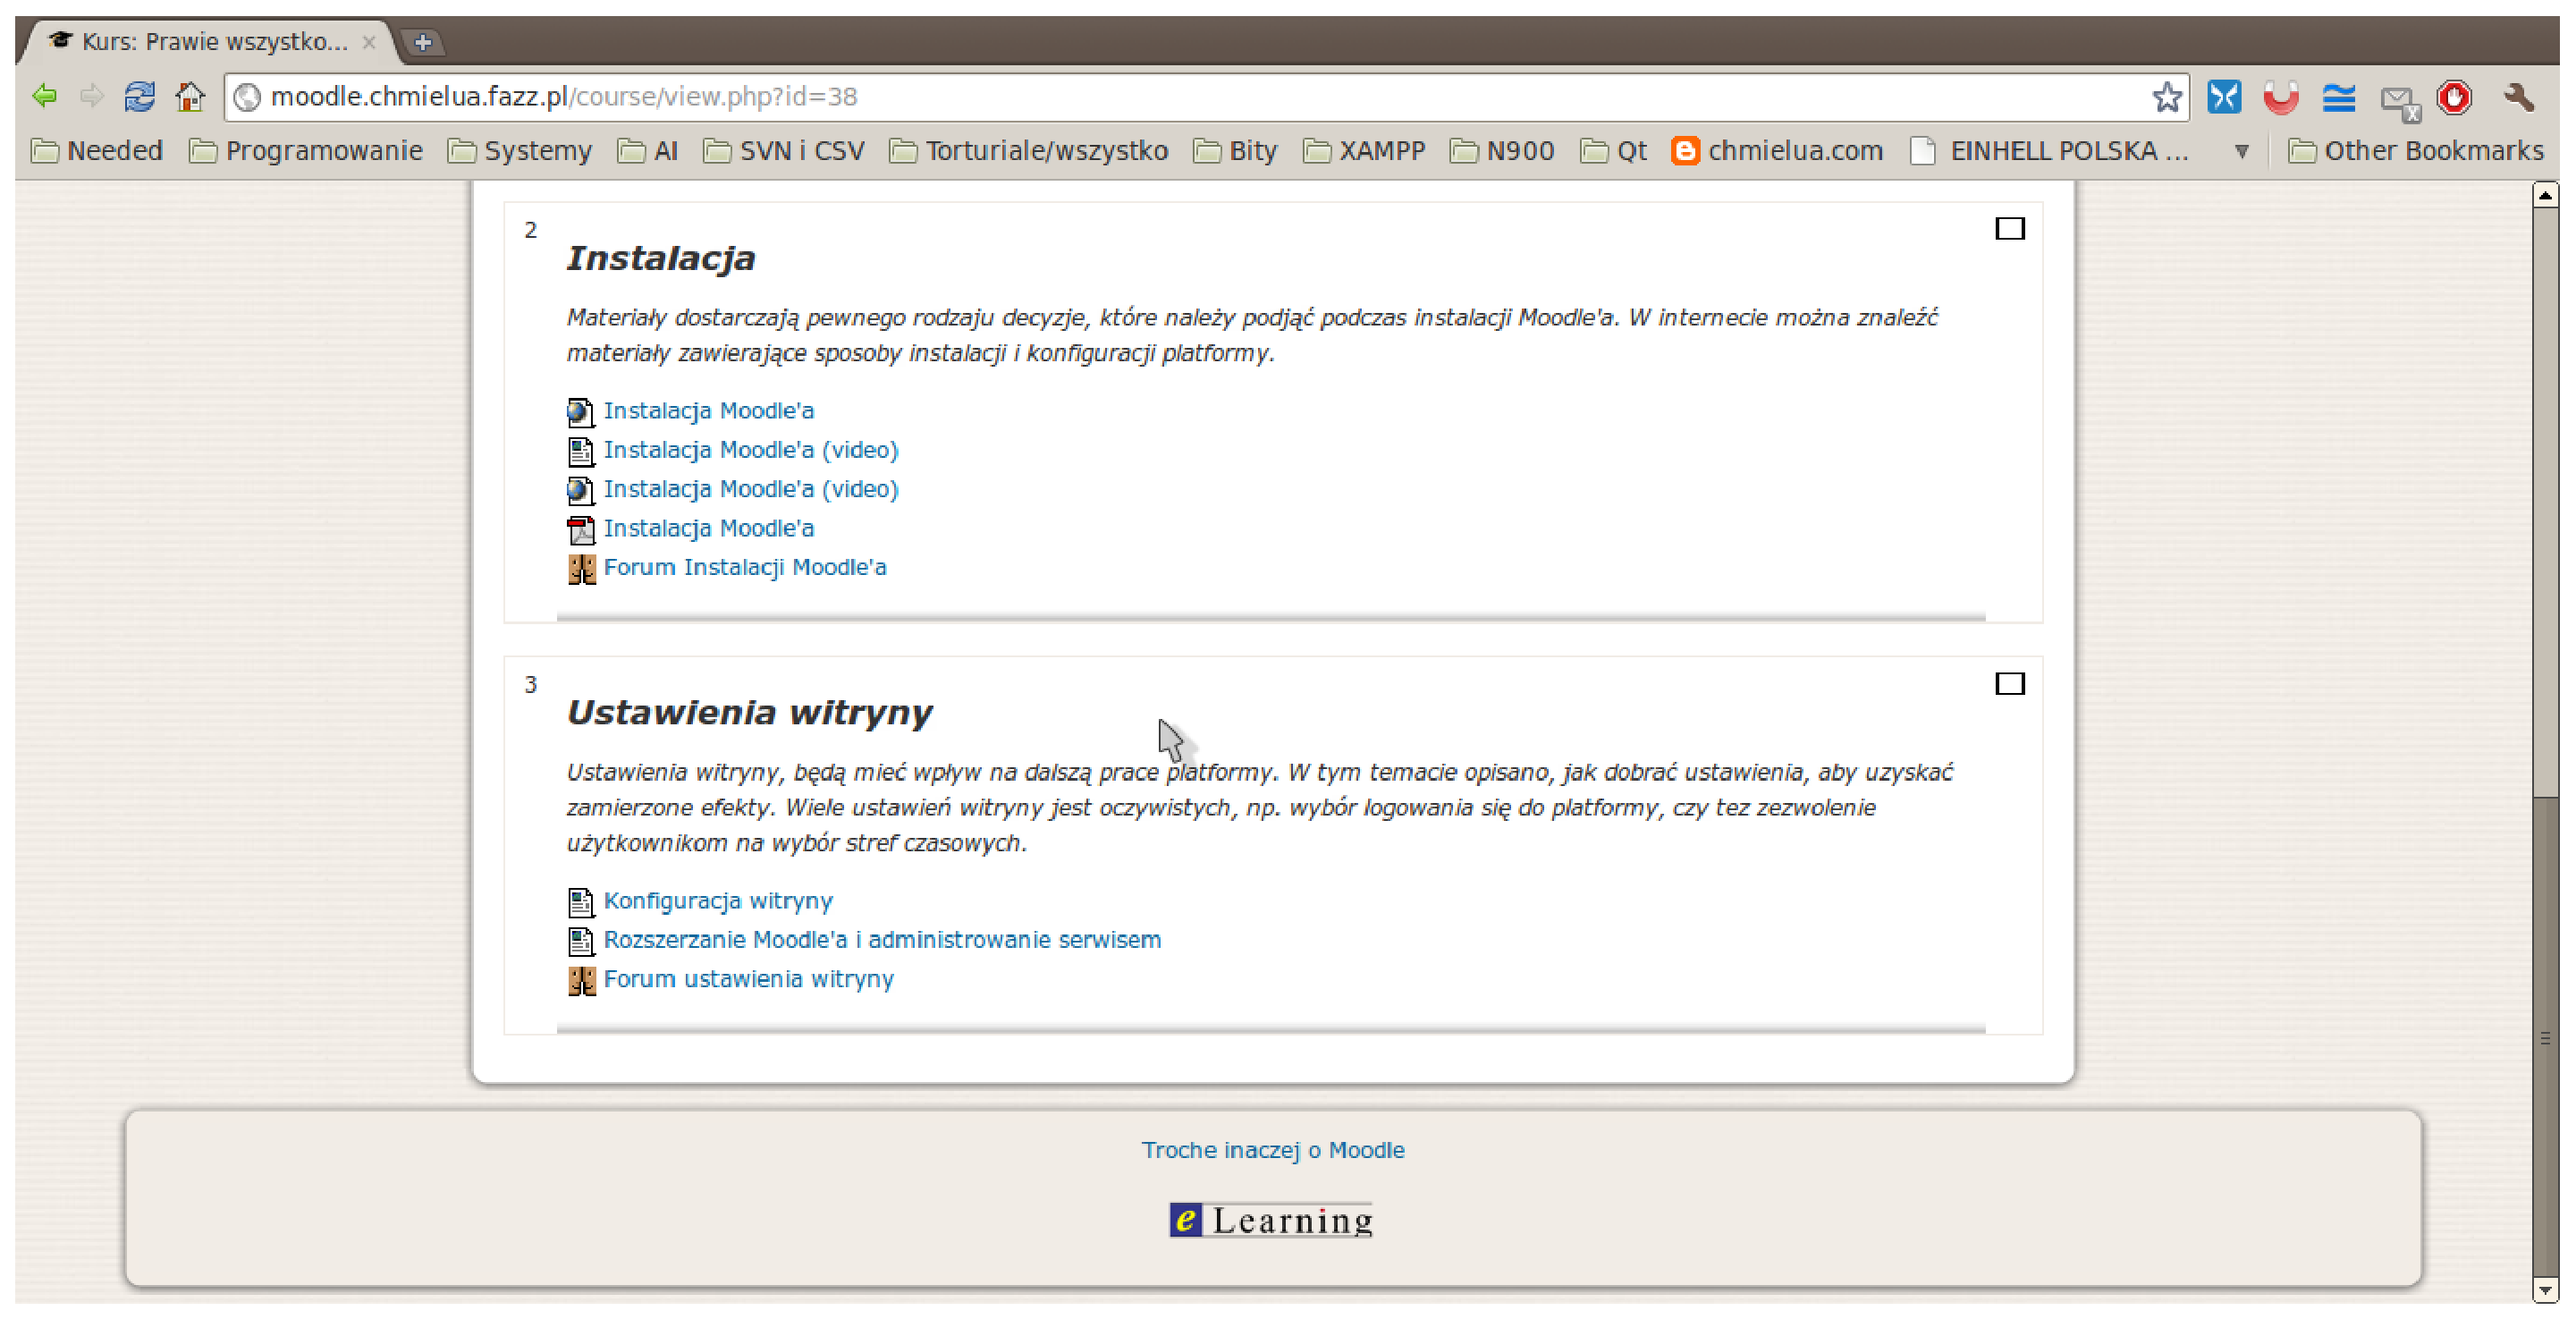
\includegraphics[width=1\textwidth]{projekt_sys//rys//kurs_moodle2.eps}
\end{figure}
Należy wybrać kurs. Przeniesie to nas do strony podzielonej na trzy tematy:
\begin{itemize}
	\item \textit{Wprowadzenie}
	\item \textit{Instalacja}
	\item \textit{Ustawienia witryny}
\end{itemize}
Rys. \ref{rys:kurs_moodle} \ref{rys:kurs_moodle2} pokazują wygląd kursu. Każdy z tematów zawiera materjały dydaktyczne w róznych formach. Na stronie widać że cały kurs posiada forum aktualności i czat. Każdy temat ma swoje osobne forum gdzie mogą być rozstrzygane problemy lub tez można dyskutować na dany temat. \\
\ \\
Administrator platformy posiada dość ciekawy zestaw narzędzi do przeglądania raportów i statystyk rys. \ref{rys:stat} dla danego użytkownika. Dzięki narzędziu GeoIP administrator jest w stanie okreslić skąd pochodziło dane logowanie. Usługa GeoIP identyfikuje pochodzenie adresu IP jak to pokazuje rys. \ref{rys:geoip}. Wynik rozpoznania pokazywany jest z wykorzystaniem narzędzia Google Map.
\begin{figure}[!h]
	\centering
		\caption{Narzędzie GeoIP} \label{rys:geoip}
		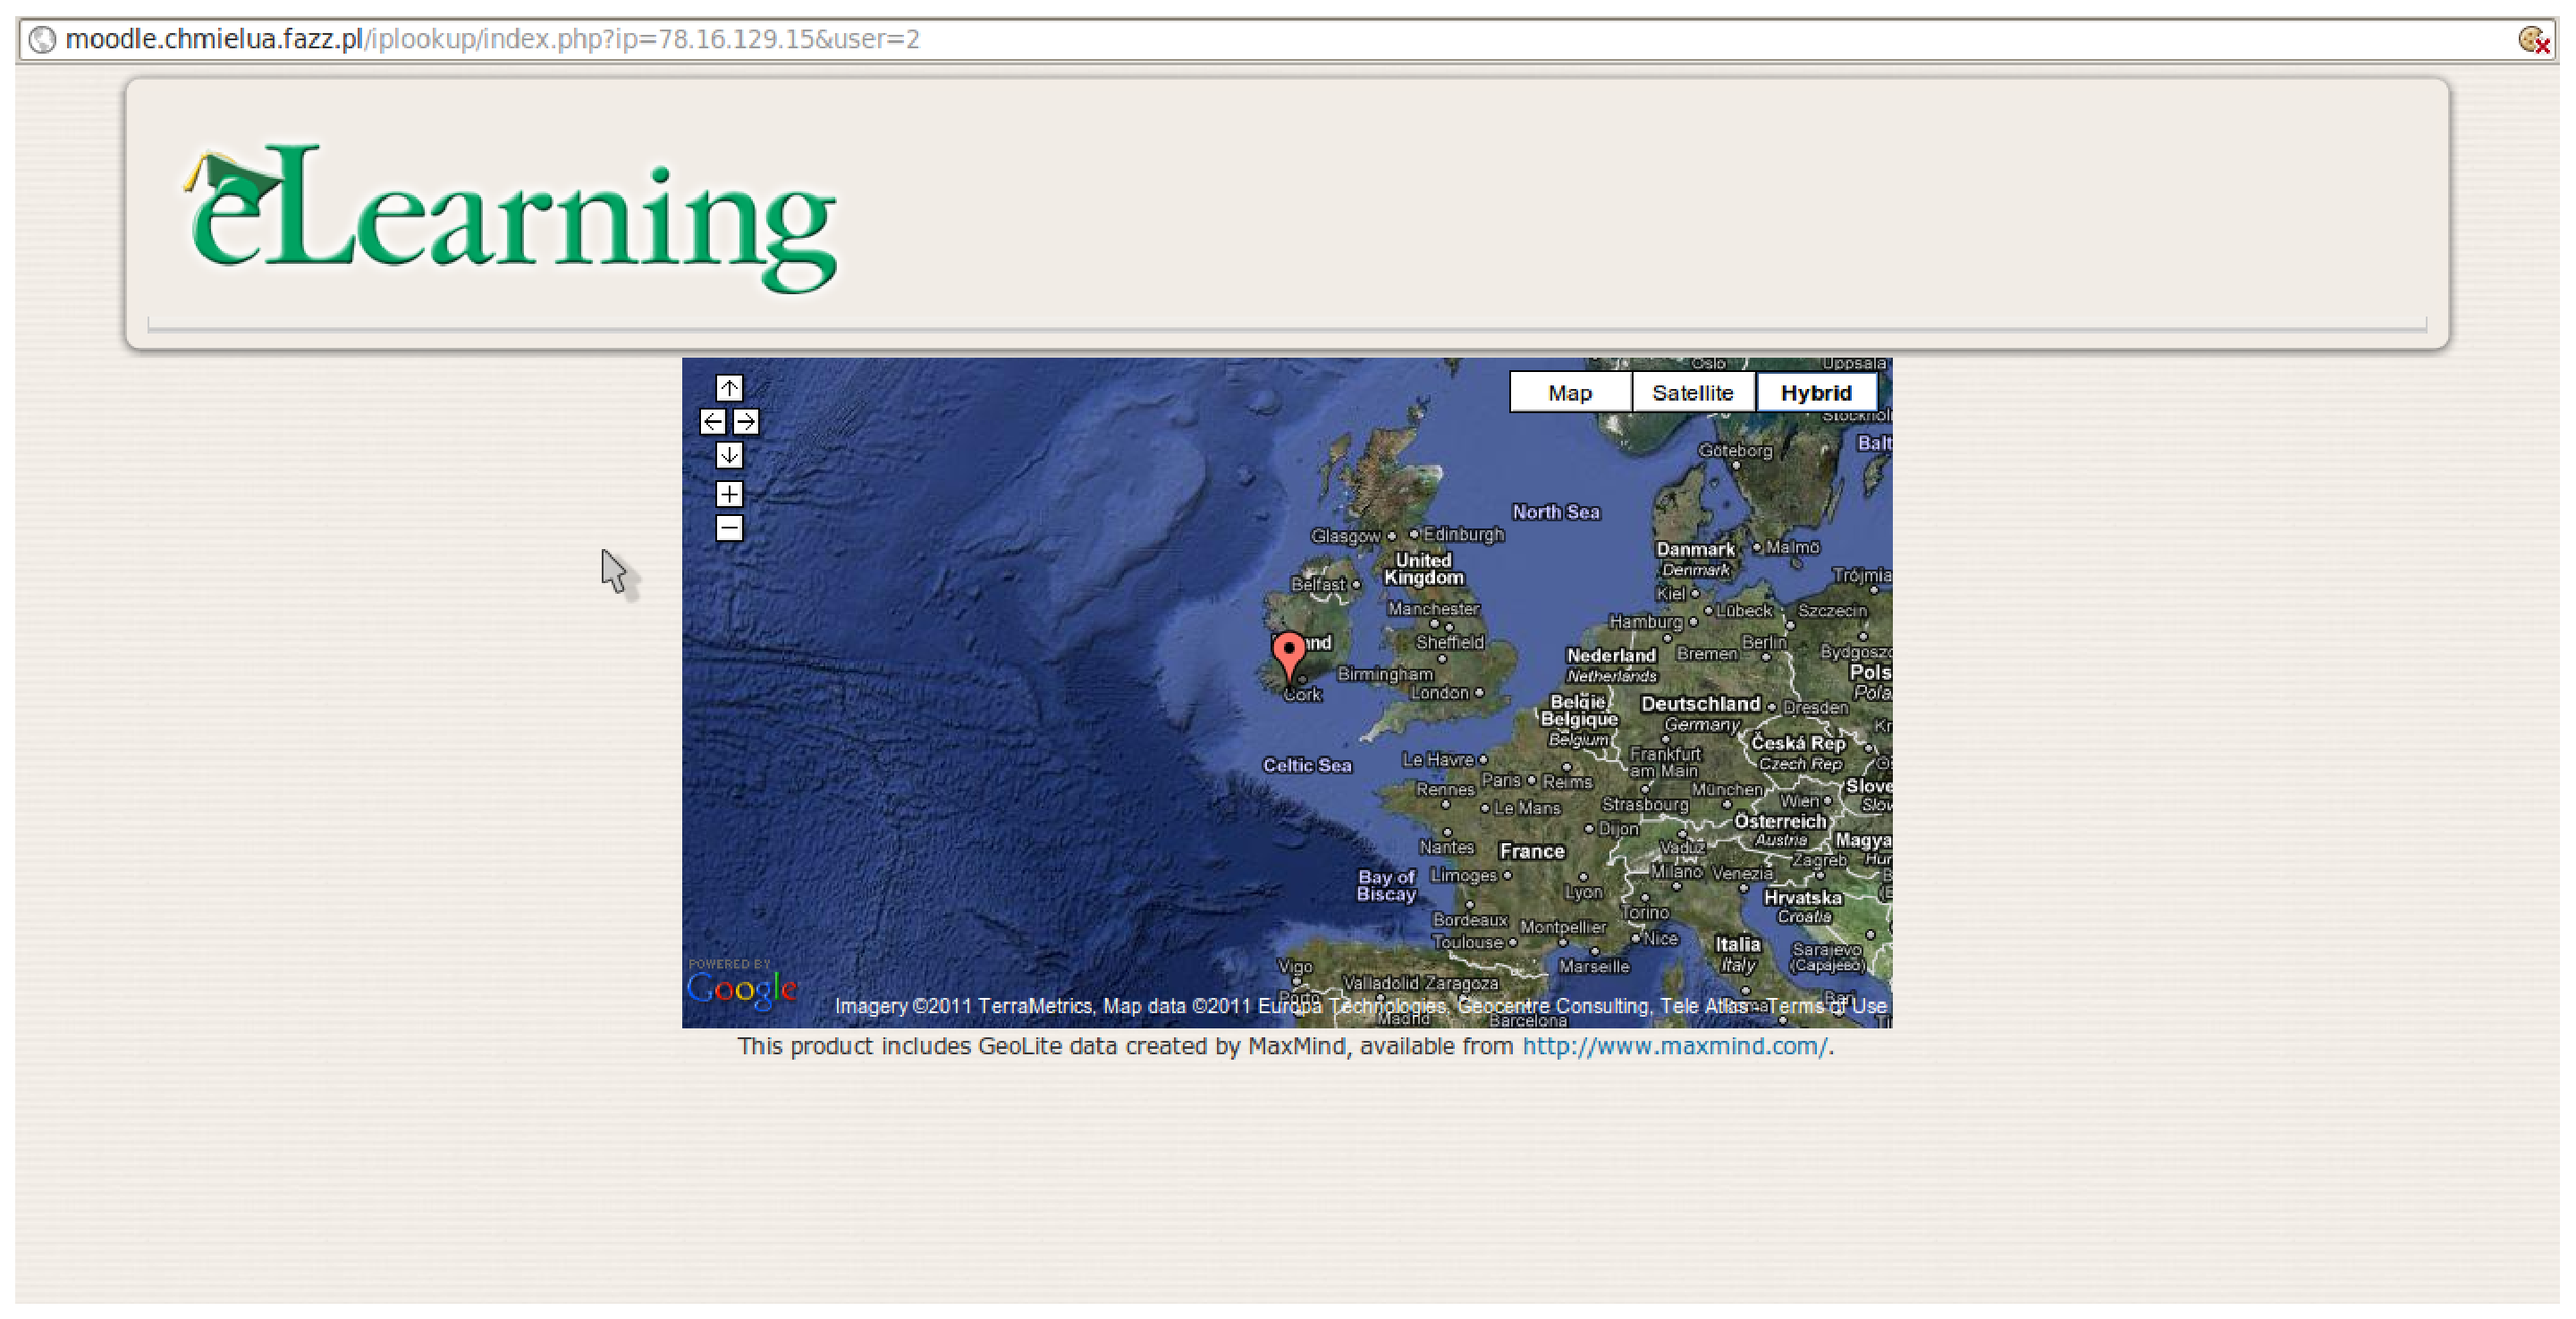
\includegraphics[width=1\textwidth]{projekt_sys//rys//geoip.eps}
\end{figure}
\begin{figure}[!h]
	\centering
		\caption{Przykładowe statystyki} \label{rys:stat}
		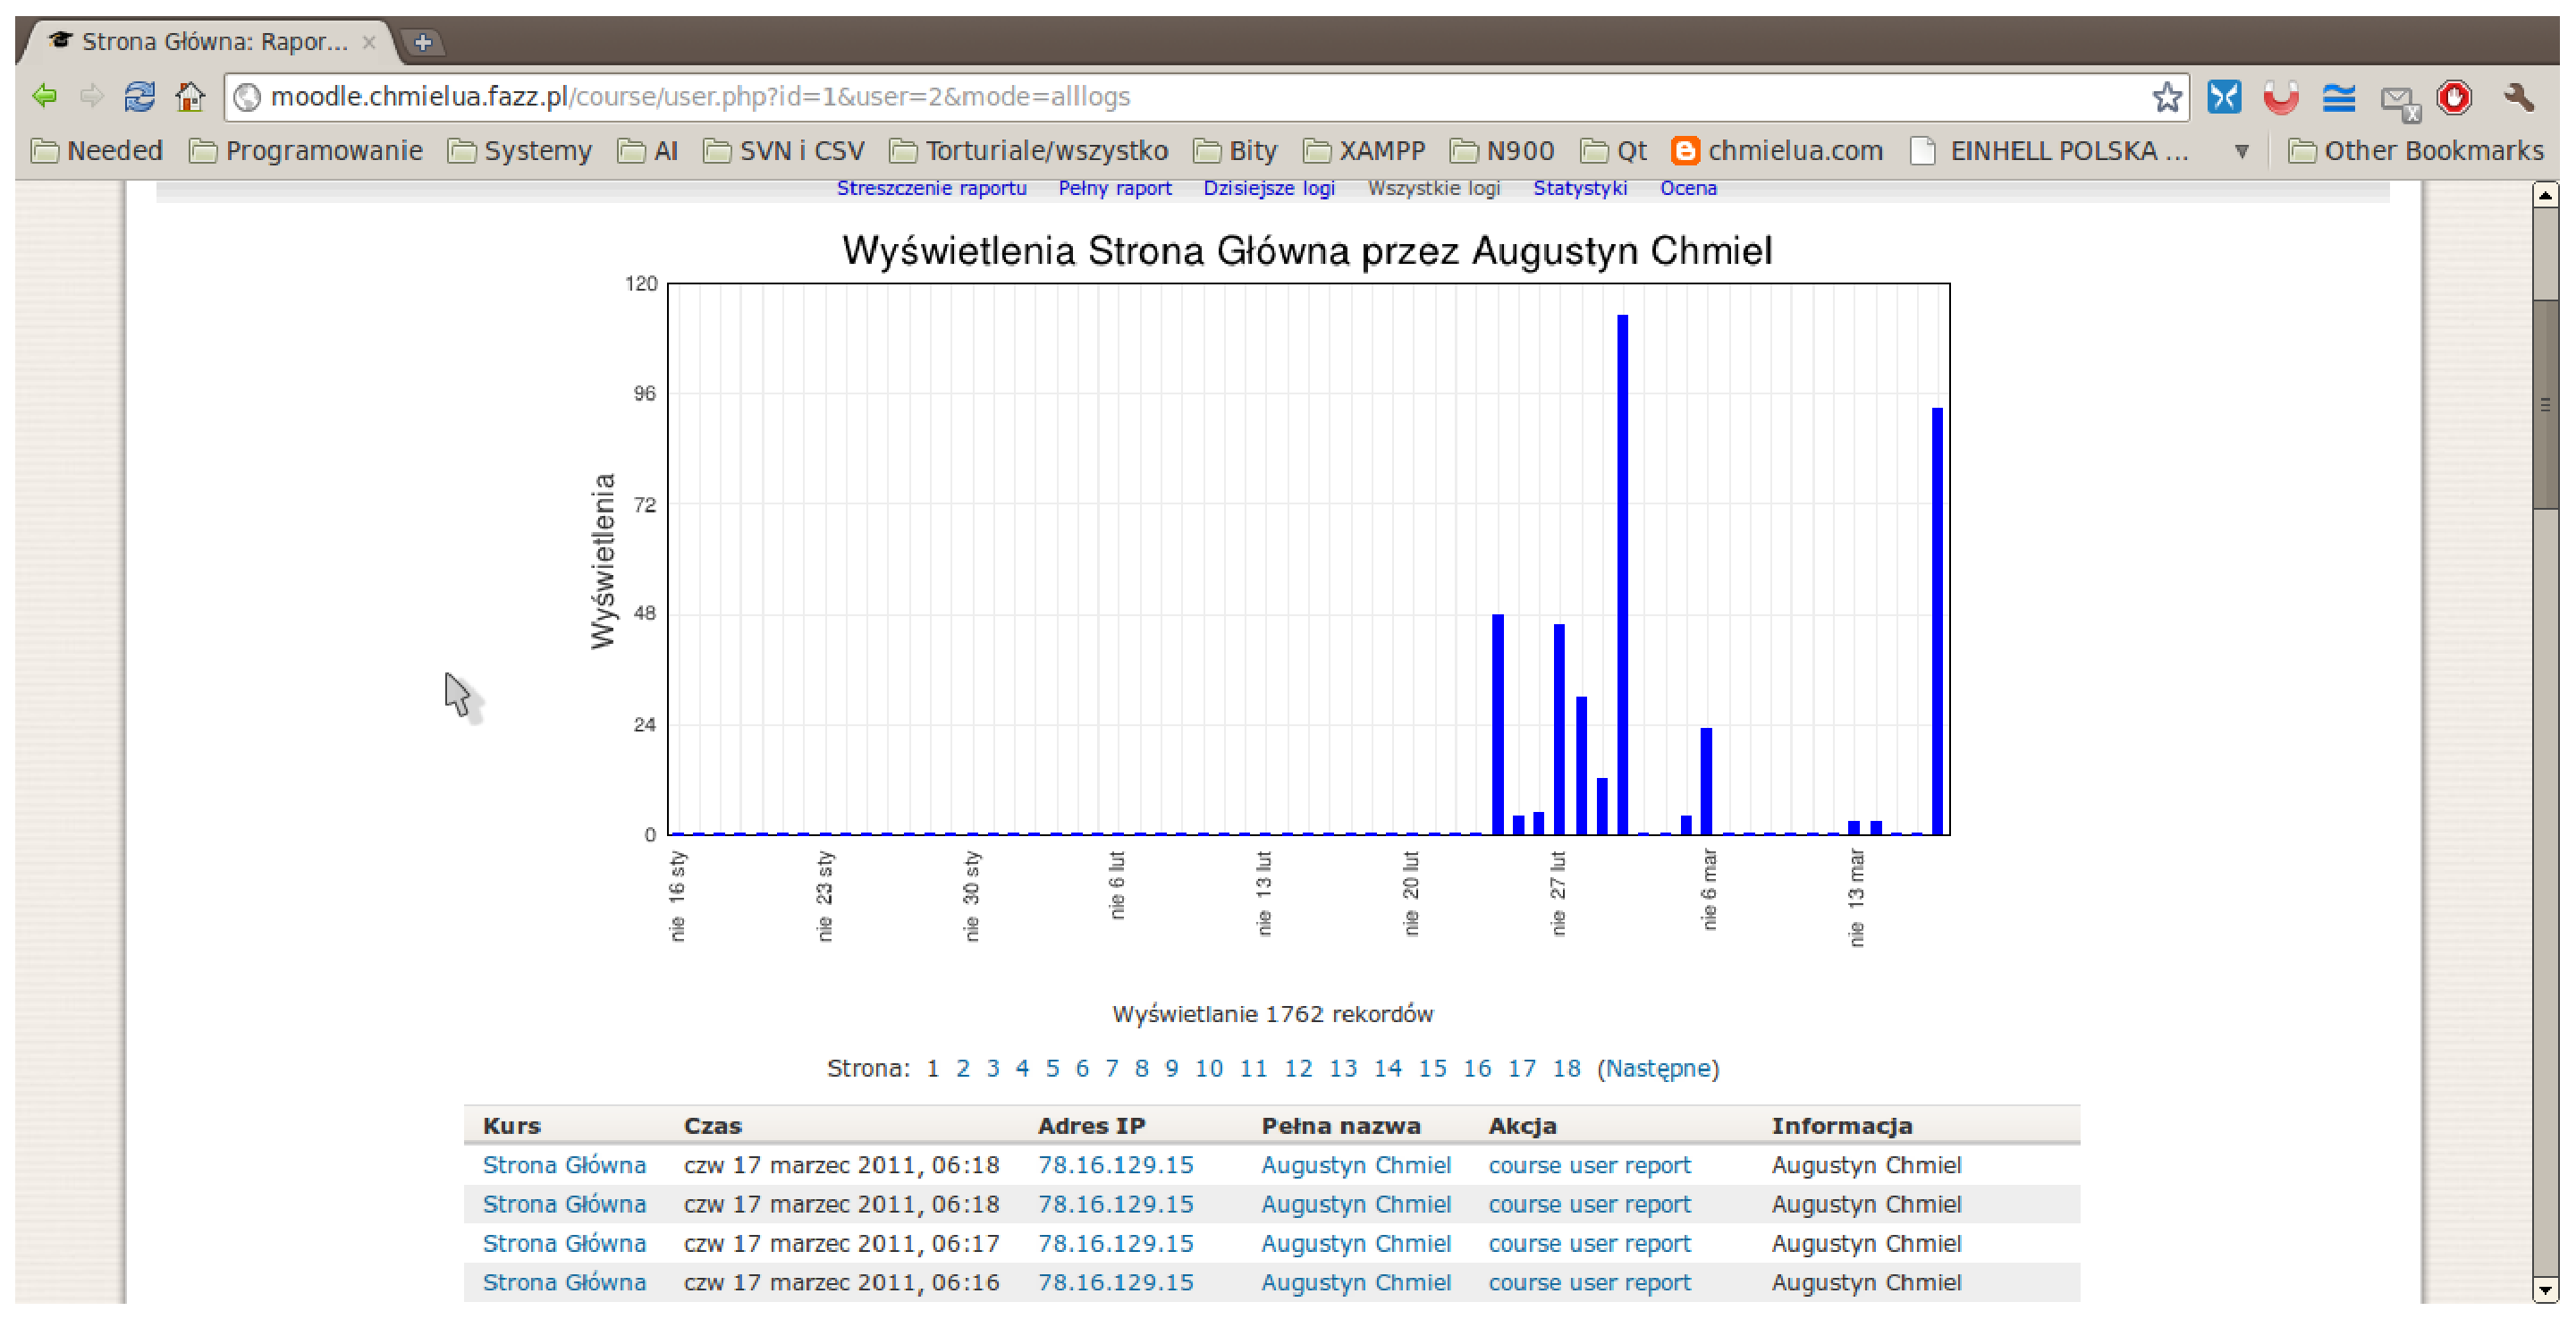
\includegraphics[width=1\textwidth]{projekt_sys//rys//stat.eps}
\end{figure}
\section{Konfiguracja witryny} \label{roz:konfig}
Z menu administracji korzystamy najczęściej podczas tworzenia witryny, w późniejszym czasie korzystamy z niego od czasu do czasu, poprawiając lub też całkiem zmieniając działanie platformy. Aby jednak mieć dostęp do menu administracyjnego trzeba skorzystać z konta administratora. Będąc zalogowanym jako administrator jesteśmy w stanie wpływać na sposób korzystania z witryny przez użytkowników. \\
\ \\
\textbf{Uwierzytelnianie} \\
\ \\
Poprzez uwierzytelnianie rozumiemy sposób logowania się do systemu. I to w jaki sposób system będzie potwierdzał tożsamość logującego się użytkownika. W Moodle'u jest udostępnionych wiele sposobów uwierzytelniania użytkowników. Ich lista znajduje się w rys. \ref{rys:blok_administracji} \textit{Administracja serwisu/Użytkownicy/Uwierzytelnianie/Zarządzaj uwierzytelnianiem} każda z tych opcji jest pokrótce objaśniona po kliknięciu \textit{Ustawienia} rys. \ref{rys:info_uwierz}.
\begin{figure}[!h]
	\centering
		\caption{Blok Administracji serwisu} \label{rys:blok_administracji}
		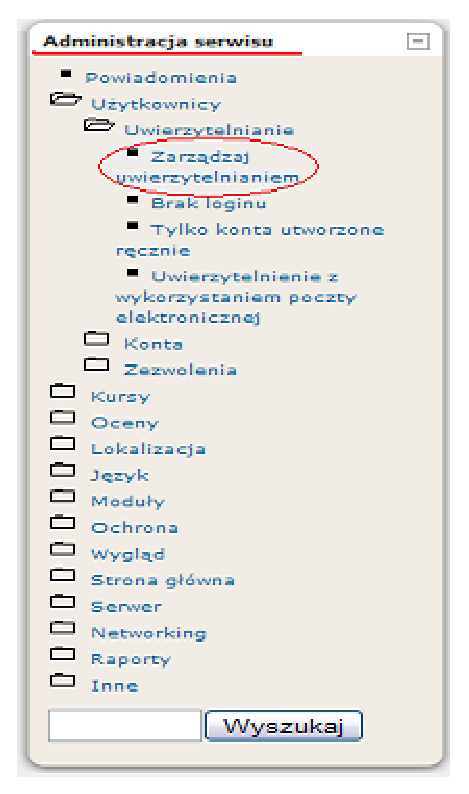
\includegraphics[width = 208px]{projekt_sys//rys//admin.eps}
\end{figure}
\begin{figure}[!h]
	\centering
		\caption{Zarządzanie uwierzytalnianiem} \label{rys:info_uwierz}
		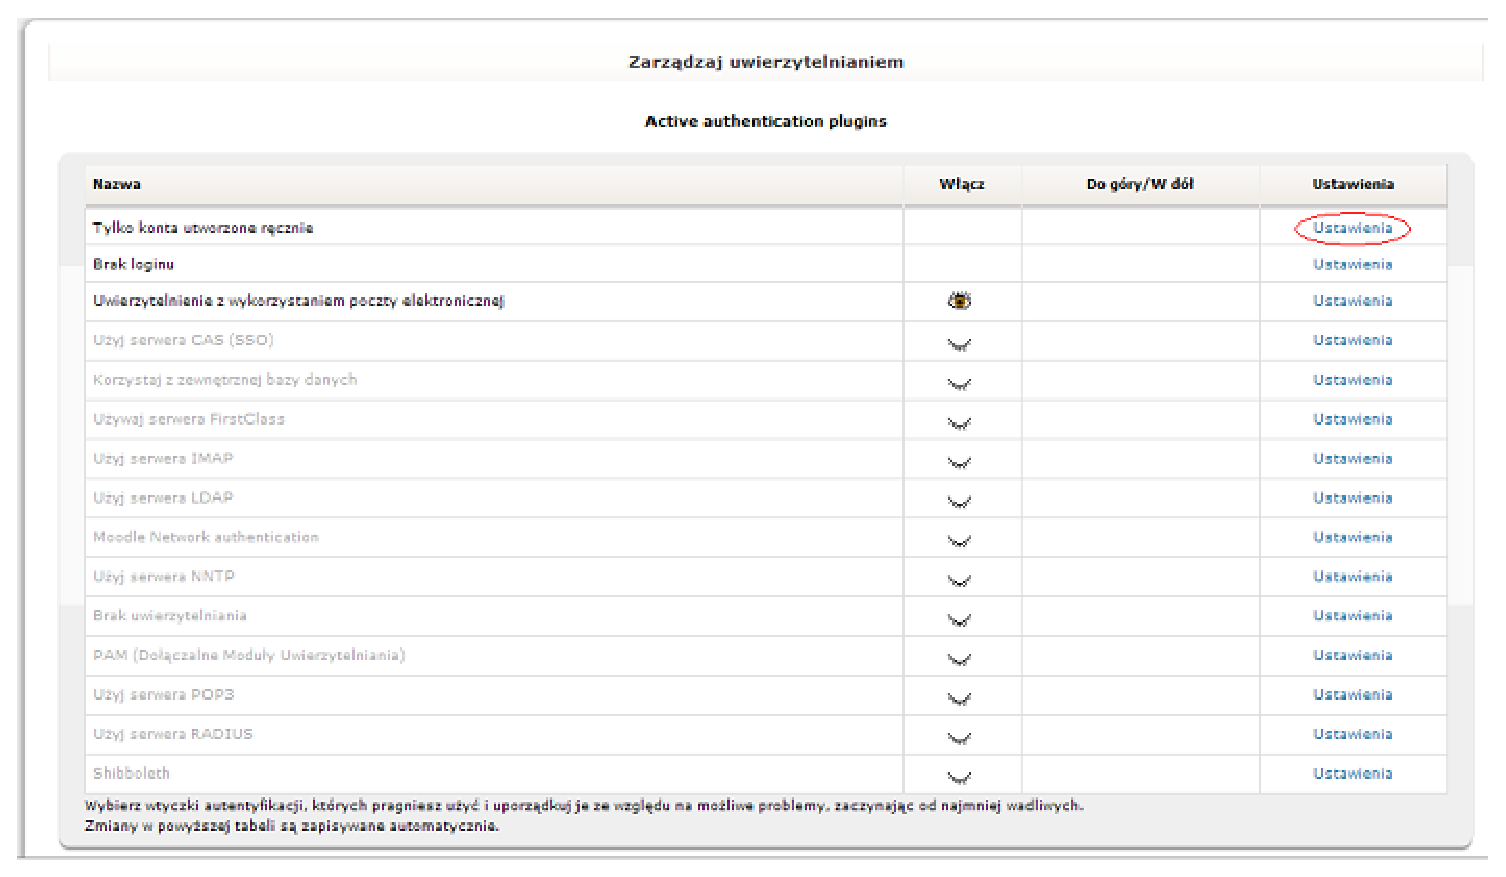
\includegraphics[width=1\textwidth]{projekt_sys//rys//uwierz.eps}
\end{figure}
\textbf{Uwierzytelnianie przy użyciu zewnętrznej bazy danych lub zewnętrznego serwera.}\\
\ \\
W przypadku uwierzytelniania za pomocą zewnętrznej bazy danych hasła można przechowywać na dwa sposoby: \\
\begin{enumerate}
	\item Moodle może tworzyć kopie danych zawartych w zewnętrznej bazie danych, w ustawieniach zewnętrznej bazy danych możemy decydować jak często ma dochodzić do mapowania danych. Teraz gdy użytkownik będzie się logować uwierzytelnianie użytkownika będzie się odbywać z użyciem wewnętrznej bazy danych.
	\item Moodle może również korzystać z zewnętrznej bazy danych przy każdym logowaniu. Przy takim stanie rzeczy Moodle nie przechowuje danych użytkownika w swojej wewnętrznej bazie danych. Nie jest też możliwe zmienianie jakichkolwiek danych przy użyciu platformy. Jeżeli użytkownik będzie chciał edytować jakiekolwiek dane będzie musiał dokonać tych zmian w zewnętrznej bazie danych.
\end{enumerate}
\textbf{Zapisy} \\
\ \\
Zapisy są czymś innym niż uwierzytelnianie. Zapisy określają do jakich kursów użytkownik przynależy, zaś uwierzytelnianie odbywa się podczas logowania do platformy. Tak samo jak przy uwierzytelnianiu, przy zapisach mamy również kilka opcji jakie umożliwiają nam dołączenie do kursu. W menu \textit{Administracja witryny/kursy/zapisy} będziemy mieć listę dostępnych opcji, które po kliknięciu \textit{Modyfikuj} rys. \ref{rys:zapisy} będą pokrótce objaśnione.\\
\begin{figure}[!h]
	\centering
		\caption{Zarządzanie zapisywaniem} \label{rys:zapisy}
		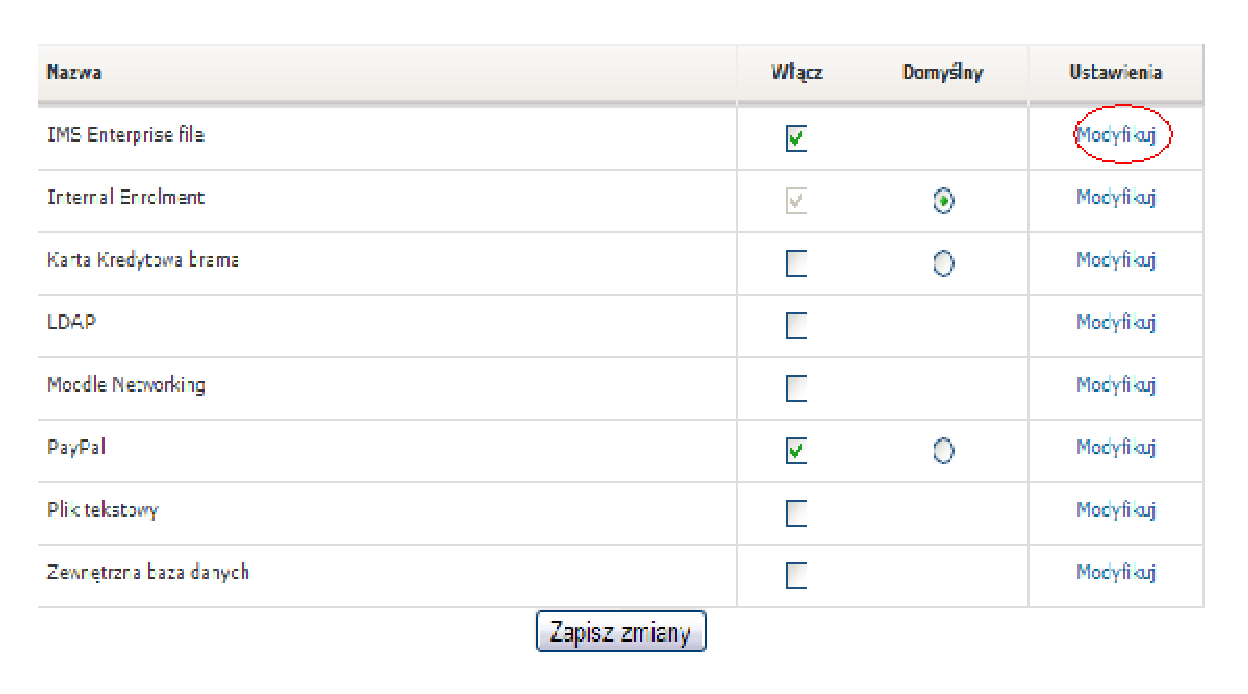
\includegraphics[width=1\textwidth]{projekt_sys//rys//zapisy.eps}
\end{figure}
\textbf{Zapisy wewnętrzne} \\
\ \\
Jest domyślną metodą zapisów. Jeżeli pozostawimy ten rodzaj zapisu, będziemy mieli możliwość zapisu ucznia, poprzez Administratora lub Nauczyciela. Innym rozwiązaniem jest opcja klucz zapisów. Jak się można domyśleć aby móc się zapisać na kurs trzeba będzie posiadać klucz.\\
\ \\
\textbf{Plik tekstowy} \\
\ \\
W przypadku zapisu większej ilości uczniów istnieje możliwość podania listy uczniów poprzez plik tekstowy. Aby móc przeprowadzić zapis poprzez plik tekstowy trzeba utworzyć plik w odpowiednim formacie. \\
\ \\
\textit{opcja, rola, identyfikator użytkownika, identyfikator kursu}\\
np.\\
\textit{add, student, 001, MOODLE01} \\
\ \\
W pliku wpisujemy skrócone nazwy ról "student" gdzie nazwa roli pisana jest wielką literą \textit{Student}. Przykład dla pliku powyżej określa nam że użytkownik o numerze \textit{001} zostanie dodany w roli ucznia do kursu o identyfikatorze \textit{MOODLE01}.\\
\begin{itemize}
	\item \textit{operacja}~-~podajemy tutaj nazwę operacji która ma być wykonana, np. \textit{add, del}
	\item \textit{rola}~-~podajemy nazwę roli jaka użytkownik będzie pełnił w kursie, \textit{student, teacher, admin}
	\item \textit{identyfikator użytkownika}~-~inaczej numer id, pole to znajduje się w profilu każdego użytkownika, aby moc skorzystać z funkcji pliku pole to musi mieć nadany identyfikator.
	\item \textit{identyfikator kursu}~-~jest to unikalny identyfikator danego kursu, może być nadawany np. podczas tworzenia kursu.
\end{itemize}
\begin{figure}[!h]
	\centering
		\caption{Numer ID użytkownika} \label{rys:nr_id}
		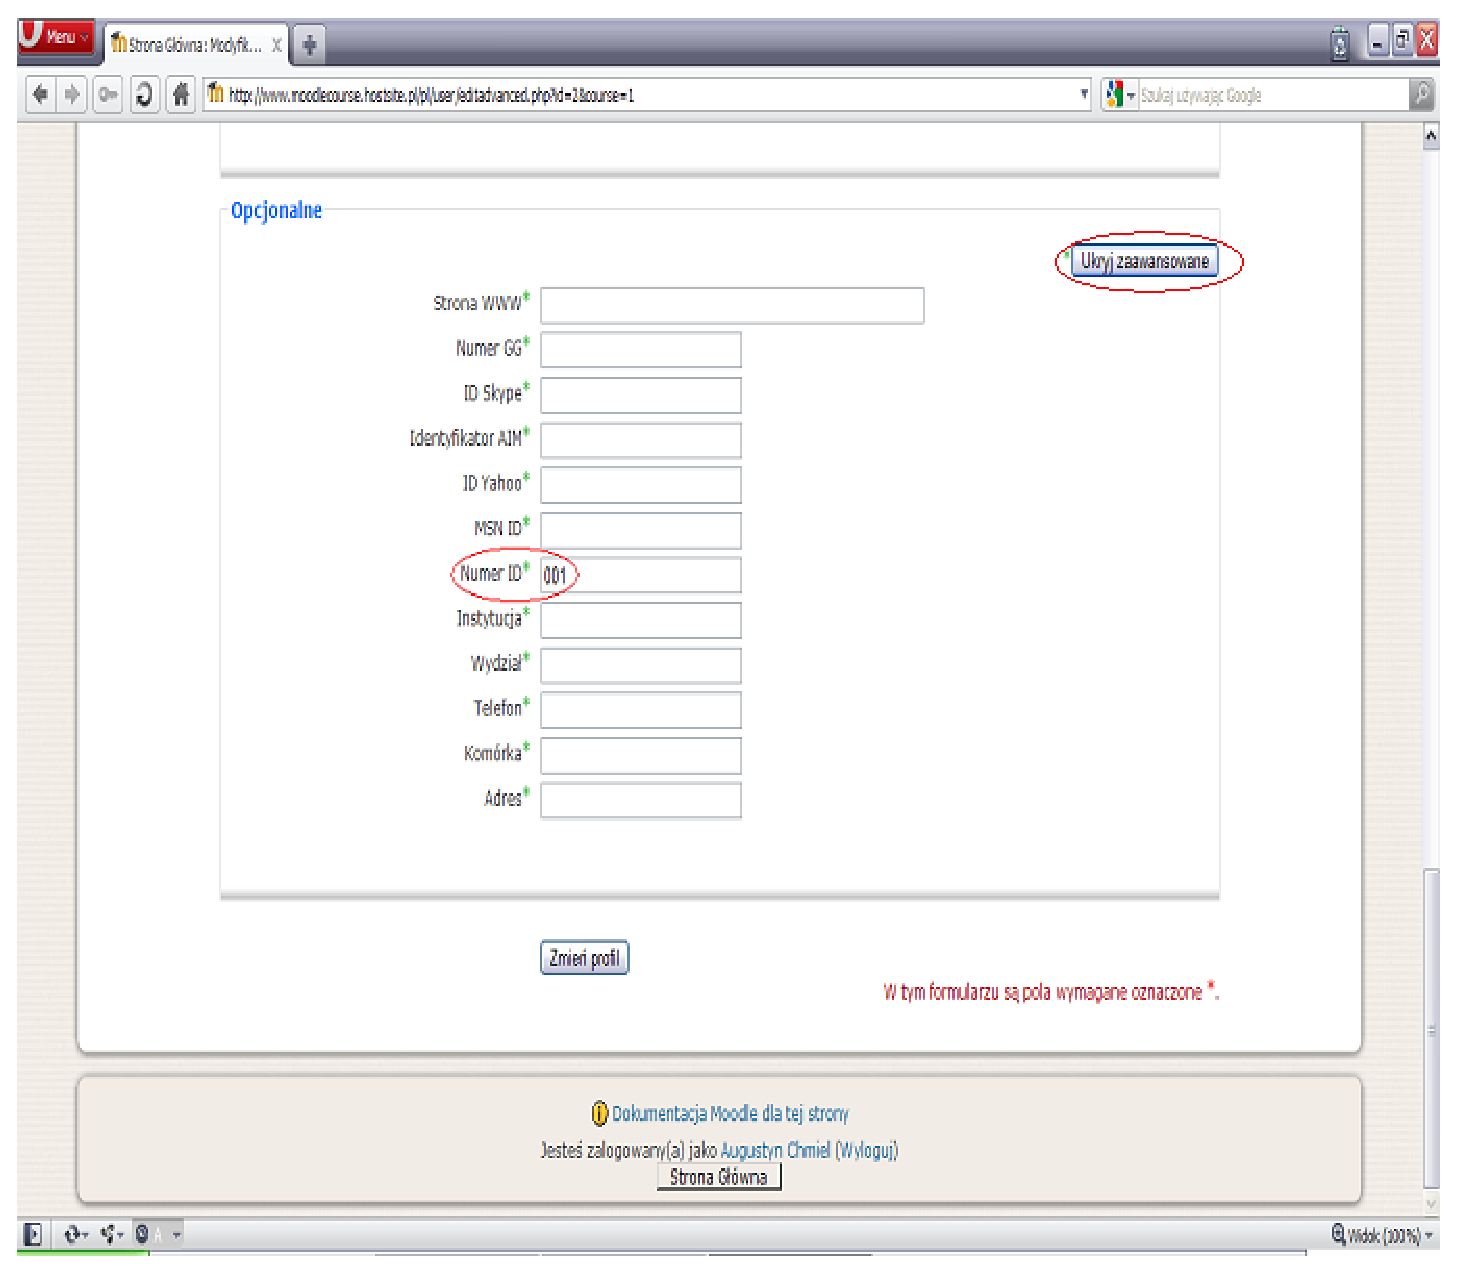
\includegraphics[width=1\textwidth]{projekt_sys//rys//nr_id.eps}
\end{figure}
Identyfikator ucznia jest wymagany przy metodzie zapisów za pomocą pliku tekstowego. W bazie danych znajduje on się w tabeli mdl\_user w kolumnie idnumber. Najszybszym sposobem wypelnienia tych pól jest zgłoszenie takiego zadania administratorowi który odpowiednia komenda SQL wypełni wszystkie pola. Na przykład coś takiego:
\begin{verbatim}
use moodle;
delimiter $

CREATE PROCEDURE id_number(id_max INT)
	BEGIN
		set @id_start = id_max - (id_max - 1);
		WHILE @id_start < id_max do
			UPDATE mdl_user SET idnumber = @id_start
                                        WHERE id = (@id_start + 1);
			set @id_start = @id_start + 1;
		END WHILE;
        END$
delimiter ;

CALL id_number((SELECT max(id) from mdl_user));
\end{verbatim}
Przydatna informacją też jest fakt że pole to jest typu VARCHAR(255) - czyli łańcuchem znaków o zmiennej długości, max 255 znaków. Również szybszym sposobem niż edycja każdego użytkownika z osobna w Moodle'u będzie skorzystanie z panelu phpMyAdmin, gdzie można w trochę szybszy sposób wyklinać wszystko i nanieś poprawki ręcznie rys. \ref{rys:baza_users},
\begin{figure}[!h]
	\centering
		\caption{Tabela użytkowników \textit{mdl\_users}} \label{rys:baza_users}
		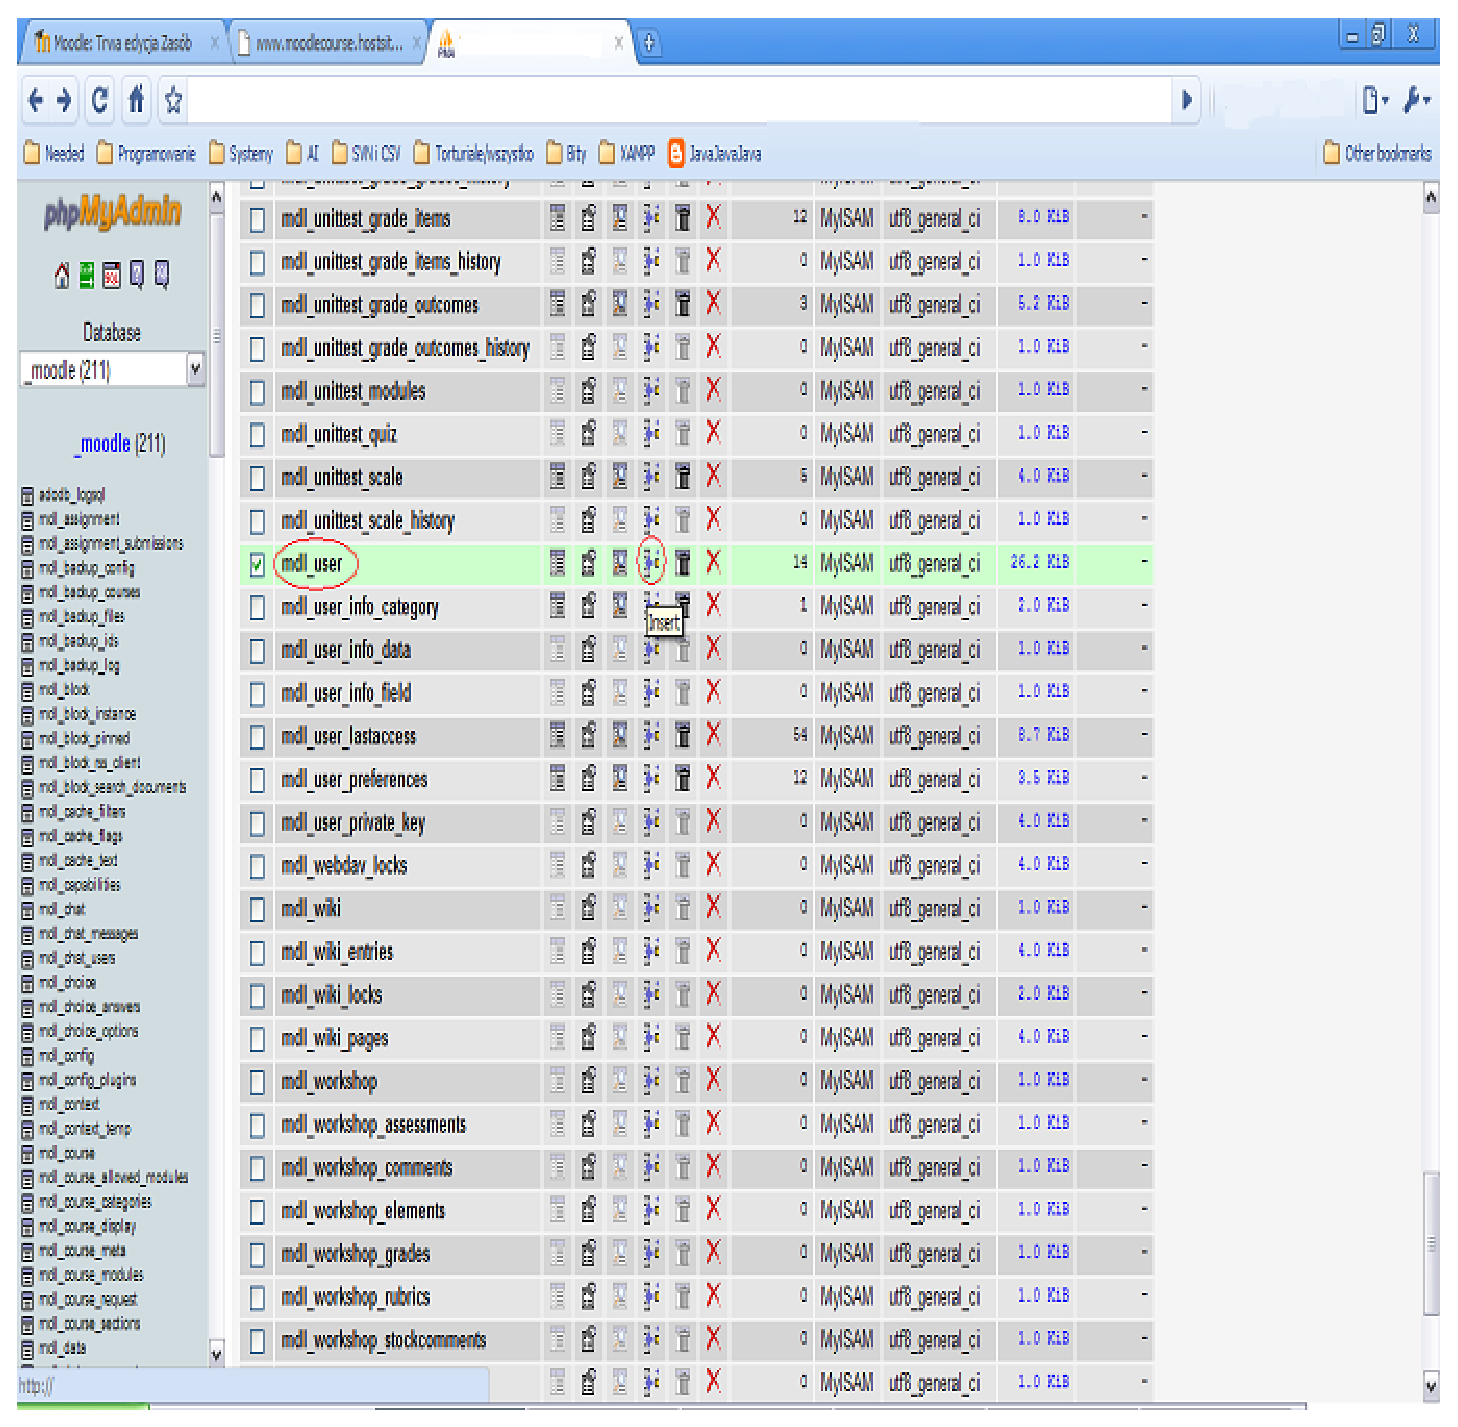
\includegraphics[width=1\textwidth]{projekt_sys//rys//baza_users.eps}
\end{figure}
\ref{rys:insert},
\begin{figure}[!h]
	\centering
		\caption{Dodanie użytkownika do \textit{mdl\_users} } \label{rys:insert}
		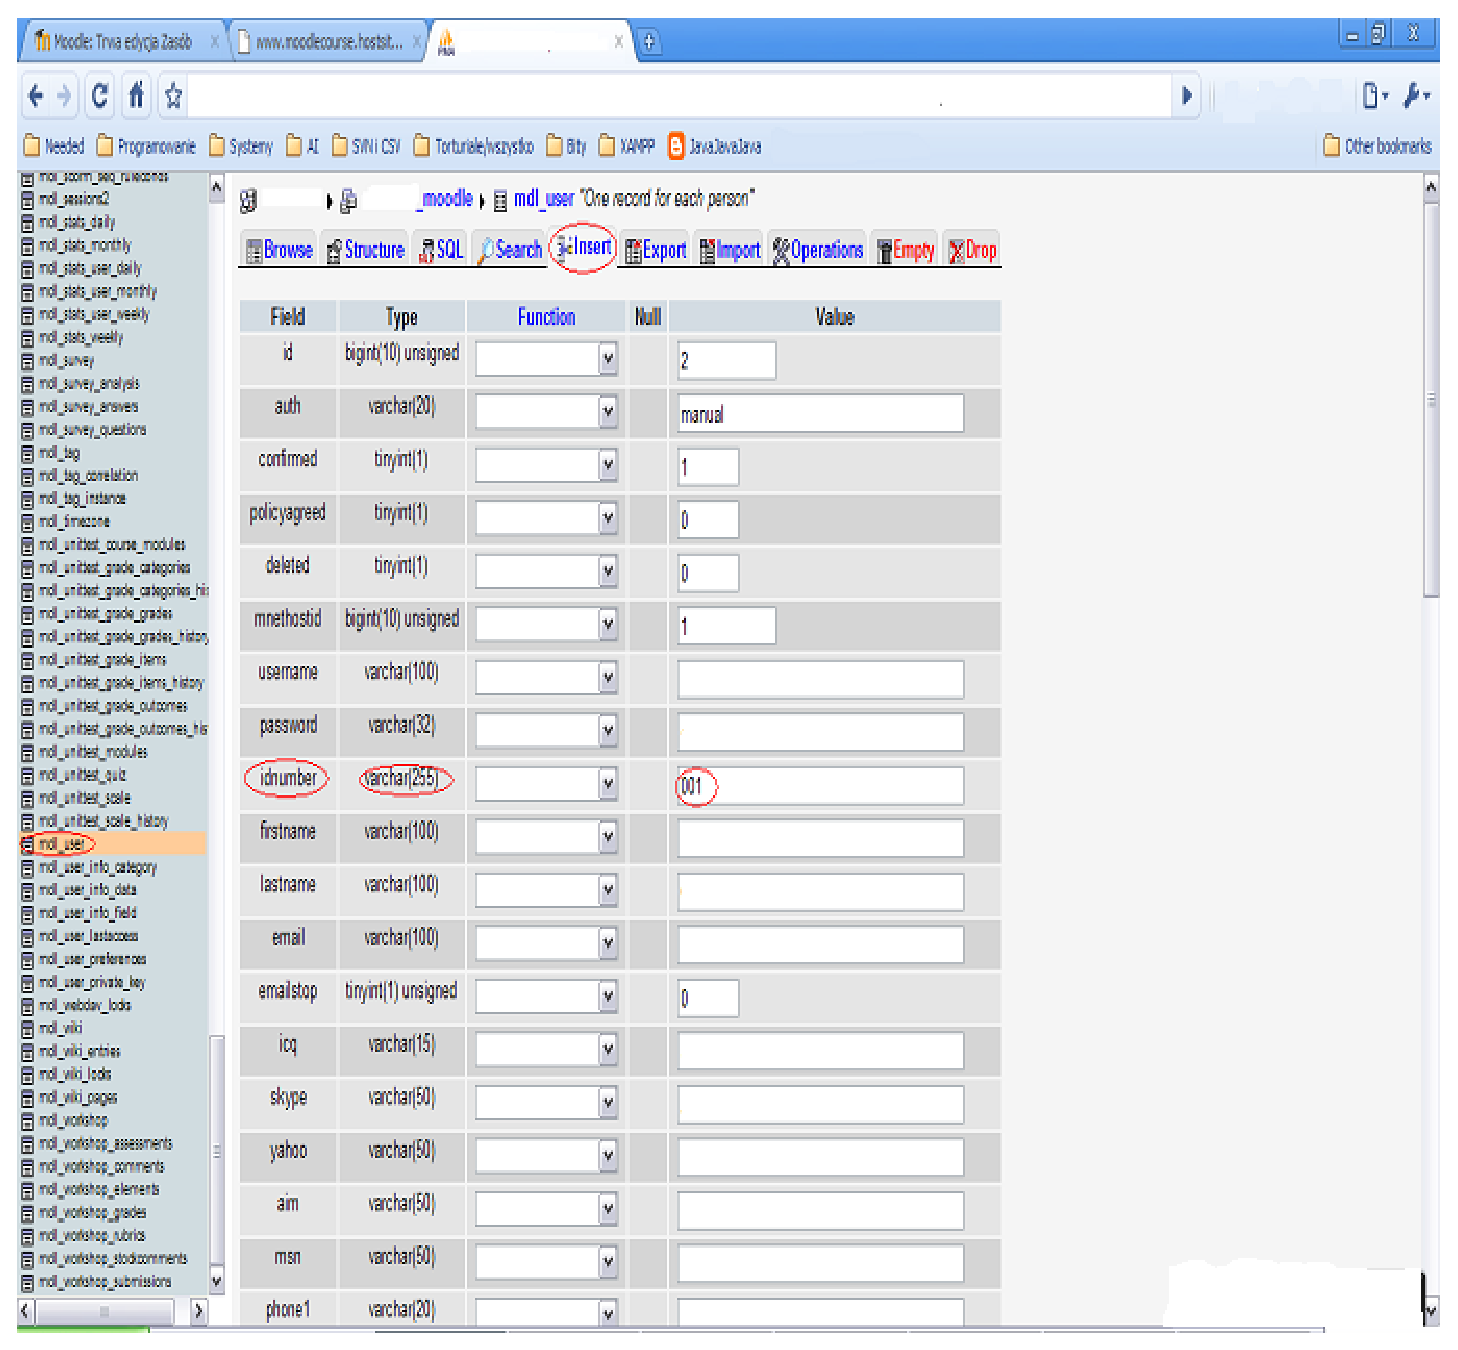
\includegraphics[width=1\textwidth]{projekt_sys//rys//insert.eps}
\end{figure}
\ref{rys:tab_user}.
\begin{figure}[!h]
	\centering
		\caption{Tabela \textit{mdl\_users}} \label{rys:tab_user}
		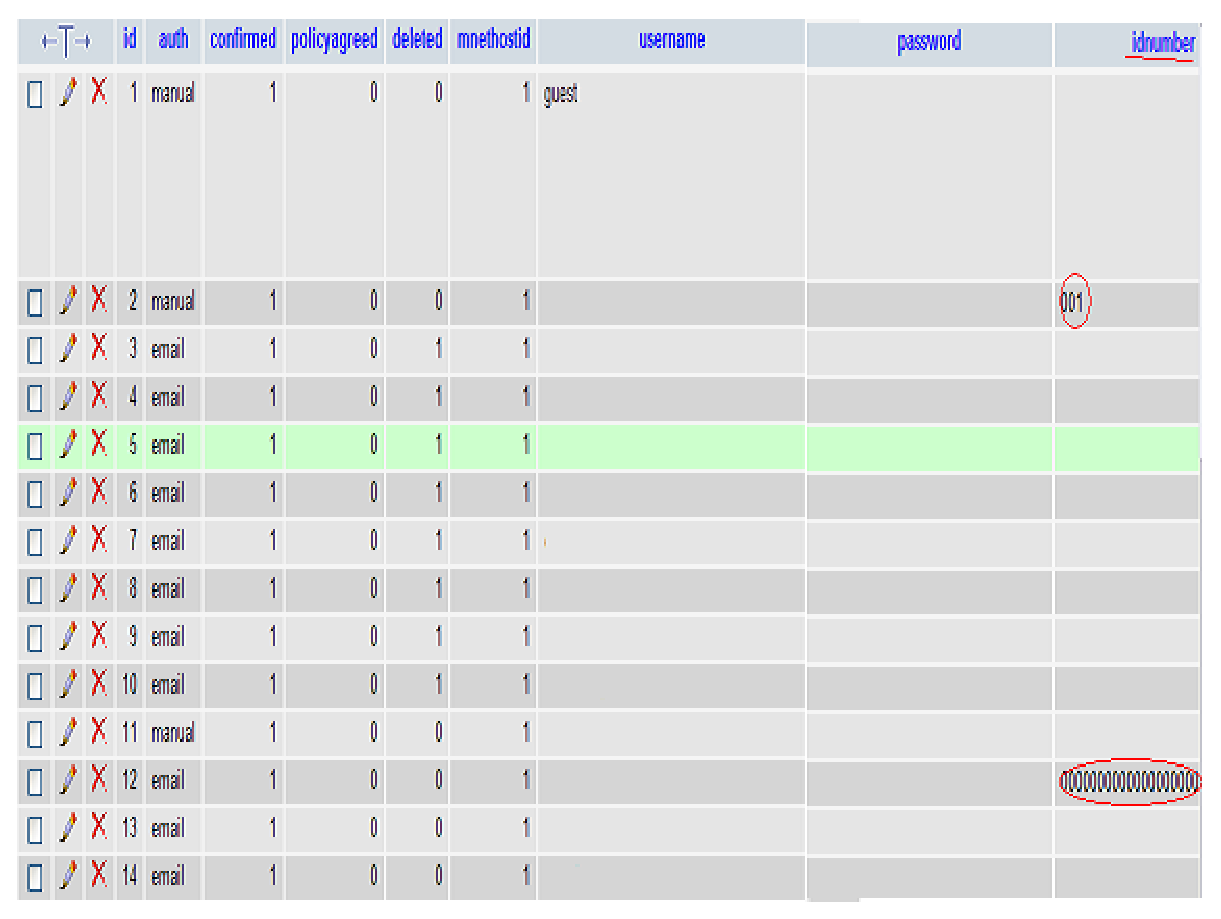
\includegraphics[width=1\textwidth]{projekt_sys//rys//tab_user.eps}
\end{figure}
A tak wygląda nasza baza po wykonaniu bardzo prostej procedury, mała rzecz, a cieszy ;) rys. \ref{rys:baza_id_users}.
\begin{figure}[!h]
	\centering
		\caption[Tabela \textit{mdl\_users} po wykonaniu procedury]{Tabela użytkowników \textit{mdl\_users} po wykonaniu procedury} \label{rys:baza_id_users}
		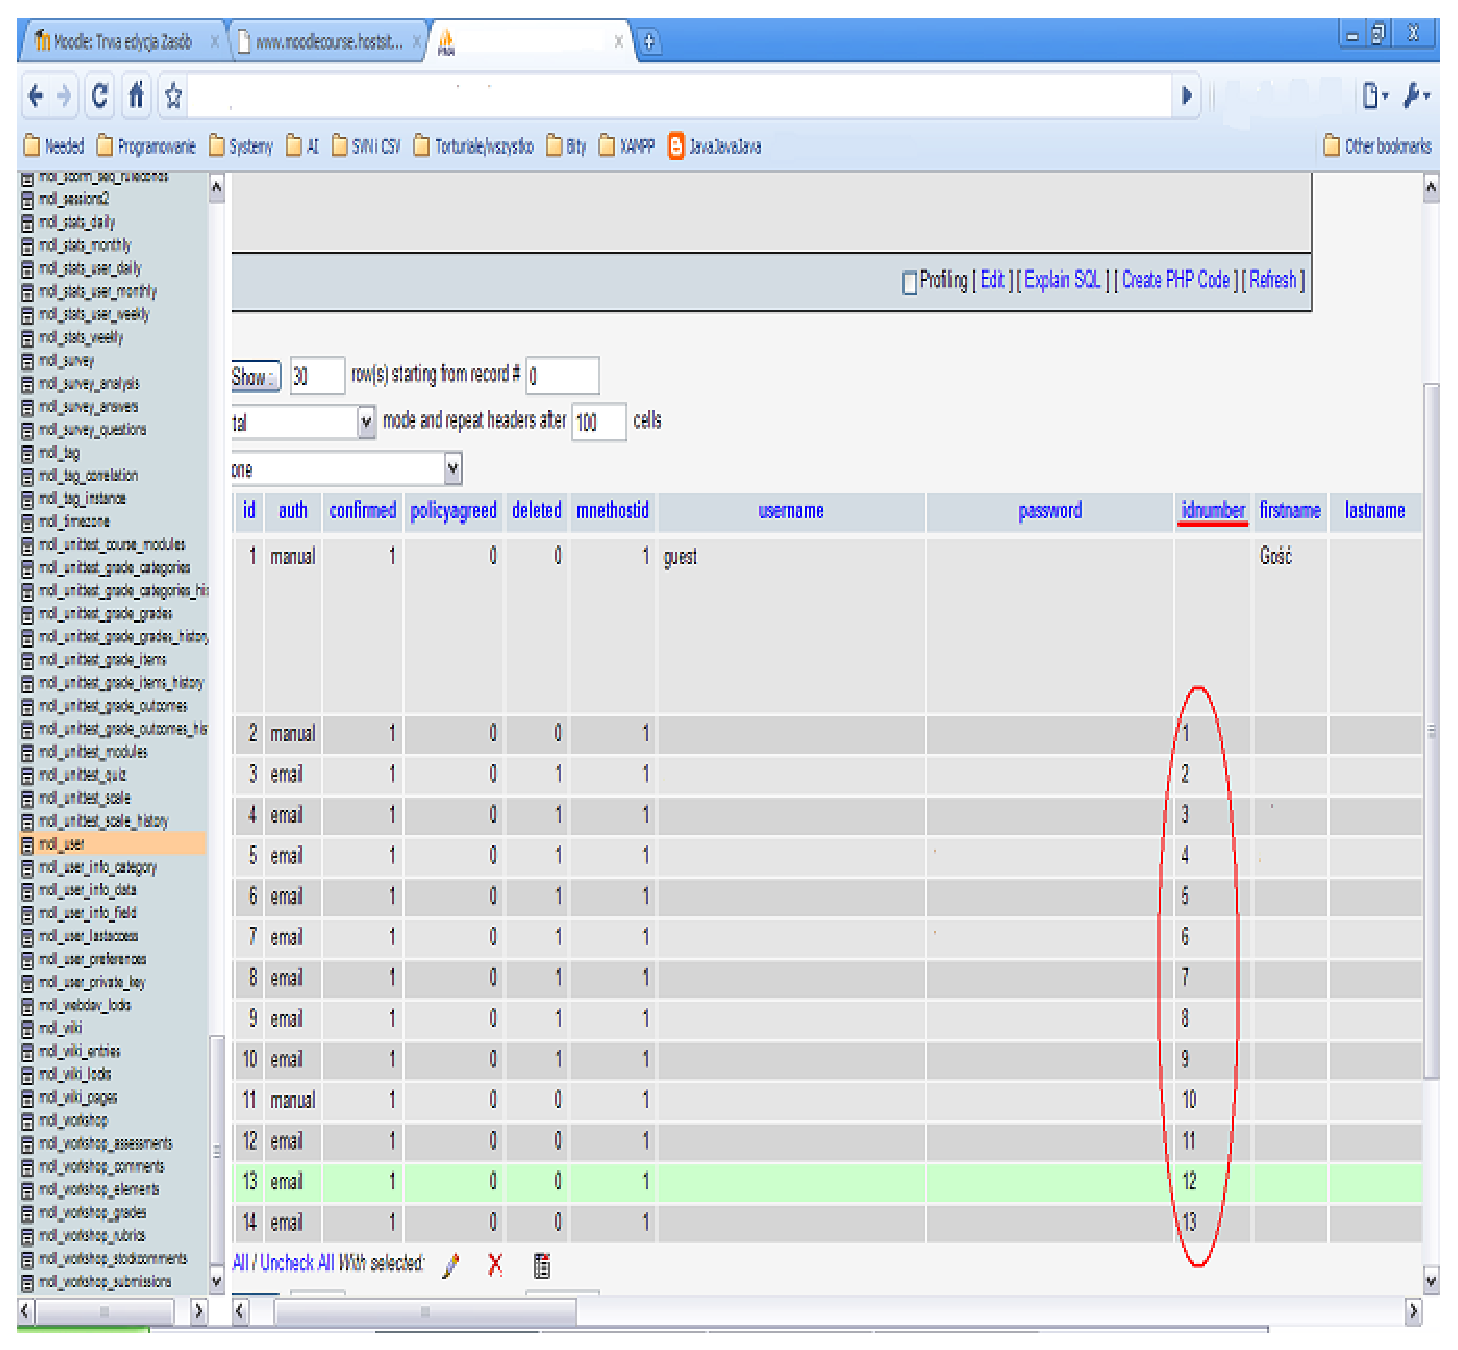
\includegraphics[width=1\textwidth]{projekt_sys//rys//procedura.eps}
\end{figure}
To jest jeden z przykładów jakiegoś tam rozwiązania można również zastosować jakiś wyzwalacz, który automatycznie po dodaniu użytkownika do tabeli nada mu jego \textit{idnumber}. Po prostu pokazuje tutaj ze można znacznie ułatwić sobie życie takimi pomysłami administrując w ten sposób platformę. \\
\ \\
Identyfikator kursu analogicznie jak to było z identyfikatorem użytkownika jest polem opcjonalnym. W bazie danych Moodle'a identyfikator kursu można znaleźć w tabeli \textit{mdl\_course} i również w kolumnie \textit{idnumber}. Tyle że w tym przypadku mamy pole typu \textit{VARCHAR(100)} czyli łańcuch o zmiennej długości, o maksymalnym zakresie 100 znaków. \\
\ \\
\textbf{Rola} \\
\ \\
Role określają nam status użytkownika, czyli mówią nam co dany użytkownik może a czego nie może. Ważnym punktem tutaj jest powiedzenie że użytkownik może mieć określoną role dla witryny, jak i również dla danego kursu i nie musi ona być taka sama jaka jest zdefiniowana dla witryny. Aby sprawdzić wszystkie domyślnie zdefiniowane role, oraz poznać ich skrócone nazwy, należy przejść do Administracja witryny/Użytkownicy/Uprawnienia/Definicje ról po wyborze roli z listy dostaniemy dokładniejsze informacje na temat roli.\\
\ \\
\textbf{Format IMS Enterprise} \\
\ \\
Jest to plik XML, który jest zgodny ze standardami okreslonymi przez \textbf{IMS Global Learning Consortium}. Pliki tego formatu maja bardzo wiele zastosowań z których głównie korzystają instytucje z systemami zarządzania zasobami ludzkimi, więcej na ten temat można znaleźć tu.\\
\ \\
\textbf{LDAP}\\
\ \\
LDAP może być wykorzystywany do zapisów jak i do uwierzytelniania, korzystając z LDAP przy zapisach, nie zmusza to nas do korzystania z niego przy uwierzytelnianiu i na odwrót.\\
\ \\
\textbf{Zewnętrzna baza danych} \\
\ \\
Moodle do obecnej wersji 1.9 nie wspiera zewnętrznej bazy danych, czyli wszystkie zmiany danych jakich trzeba dokonać w zewnętrznej bazie danych muszą być dokonywane przez inny program. Podczas korzystania z zewnętrznej bazy danych przy zapisach na kursy, możemy również korzystać z bazy wewnętrznej w Moodle'u. W ustawieniach zewnętrznej bazy danych trzeba zdefiniować pole po którym dane z wewnętrznej bazy danych będą kojarzone z bazą zewnętrzną. Mianowicie do pola o nazwie \textit{enrol\_localcoursefield} należy podać nazwę kolumny z tabeli \textit{mdl\_course}. Nazwa kolumny która nas interesuje to znów nasze \textit{idnumber} i tak samo postępujemy z następnym polem o nazwie \textit{enrol\_localuserfield} znów podajemy \textit{idnumber}.\\
\ \\
\textbf{Wybór języka}\\
\ \\
Przy wyborze języka dobrze jest się zastanowić już na samym początku tworzenia naszej platformy. Mianowicie instalacja Moodle'e zawiera wiele pakietów językowych, które służą do tłumaczenia interfejsu a nie zasobów kursu. Może się również zdarzyć że jakaś część interfejsu nie została przetłumaczona, wówczas Moodle używa domyślnie wersji językowej angielskiej. W celu dokładniejszego przetłumaczenia interfejsu można się pokusić o pogrzebanie w plikach znajdujących się w katalogu \textit{/moodledata/lang/} i tak np. dla jeżyka polskiego następnym katalogiem będzie \textit{/pl\_utf8/}. Moodle może nam podać dokładną liczbę brakujących tłumaczeń. W tym celu należy się udać \textit{Administracja/Język/Edycja języka}. Platforma posiada tłumaczenia, ale tylko i wyłącznie samych interfejsów. W celu uzyskania pełnego tłumaczenia wraz z zawartością kursów, mamy dostępne następujące opcje: \\
Utworzenie dokumentów dla danego kursu w rożnych językach, co moim zdaniem jest jakiś rozwiązaniem, ale daje dość brzydki bałagan na stronie kursu czy też w kursach. \\
\ \\
Drugą opcją jest utworzenie różnych kursów w rożnych językach.\\
\ \\
Trzecią możliwością jest utworzenie odrębnej platformy Moodle'a dla każdego języka np. \textit{http://www.moodlecourse.pl/pl/} dla języka polskiego i \textit{http://www.moodlecourse.pl/en/} dla języka angielskiego. Na stronie głównej uczniowie wybierają język i są automatycznie przekierowywani do odpowiedniej instalacji Moodle'a. Więc widzimy że chcąc udostępniać platformę w różnych językach dobrze jest rozważyć taką sytuacje przed instalacją Moodle'a. \\
\  \\
Ostatnią możliwością jest zastosowanie filtrów. Rodzaje filtrów i ich ustawienia znajdziemy tu: \textit{Administracja/Moduły/Filtry/Filtruj} ustawienia następnie należy włączyć filtr o nazwie treść wielojęzyczna, aby nasz filt prawidłowo zadziałał należy umieścić tekst w znacznikach \textit{<spam>} w następujący sposób:\\
\begin{verbatim}
<span lang = "en">English Course</span>
<span lang = "pl">Polski kurs</span>   
\end{verbatim}
\section{Plan tworzenia witryny nauczania} \label{roz:plan}
W tym podrozdziale przedstawie liste zadan jakie należy wykonać, aby utworzyć witryne nauczania z wykorzystaniem platformy Moodle (źródło: \cite{tworzenie_serwisow}):
\begin{enumerate}
	\item Planowanie kursu.
	\begin{description}
		\item[a)] Określenie celów nauczania~-~należy określić jąką wiedze mają posiąść użytkownicy w trakcie kursu.
		\item[b)] Zbieranie materiałów do kursu. 
		\item[c)] Zastanowienie się nad ideą konstrukcjonizmu społecznego. Zaplanowanie sposobu nauki online pozwalającego na eksplorację i instalację.
	\end{description}
	\item Instalacja i konfiguracja Moodle'a.
	\begin{description}
		\item[a)] Instalujemy Moodle'a...
		\begin{itemize}
			\item Otrzymanie uprawnień na serwerze, który spełnia wymagania Moodle'a.
			\item Utworzenie poddomen i/lub katalogów potrzebnych do instalacji Moodle'a i do przechowywania jego danych.
			\item Pobranie i rozpakowanie Moodle'a oraz przesłanie go na serwer.
			\item Utworzenie katalogu danych Moodle'a.
			\item Utworzenie bazy danych Moodle'a.
			\item Ustawienie zadań corna.
			\item Aktywacja instalacji.
		\end{itemize}
		\item[b)] Jeżeli administrujemy witrynę lub tworzymy kursy...
		\begin{itemize}
			\item Konfiguracja zmiennych dla całej witryny.
			\item Konfiguracja ustawien dla całej witryny.
			\item Konfiguracja uwierzytelniania i kopii zapasowych.
		\end{itemize}
	\end{description}
	\item Tworzenie struktury witryny nauczania.
	\begin{description}
		\item[a)] Tworzenie i porządkowanie kategorii kursów.
		\item[b)] Tworzenie kursów.
		\begin{itemize}
			\item Konfiguracja ustawień kursu.
			\item Porządkowanie kursów w kategoriach.
			\item Przypisywanie ról nauczycielom.
		\end{itemize}
		\item[c)] Wybieranie bloków do wyświetlaniaw całej witrynie.
		\item[d)] Wybieranie bloków do wyświetlania w poszczególnych kursach.
	\end{description}
	\item Dodawanie podstawowego materiału do kursów.
		\begin{description}
			\item[a)] Dodawanie materiałów do czytania: stron tekstowych i internetowych.
			\item[b)] Dodawanie odnośników do innych witryn.
			\item[c)] Tworzenie katalogów plików i przesyłanie plików do nich.
			\item[d)] Porządkowanie materiału w tematy lub tygodnie.
			\item[e)] Dodawanie etykiet.
			\item[f)] Dodawanie bloku \textit{Activities (elementy interaktywne)}, jeżeli jest potrzebny.
		\end{description}
	\item Tworzenie elementów interaktywnych.
		\begin{description}
			\item[a)] Dodawanie zadań.
			\item[b)] Dodawanie głosowań.
			\item[c)] Dodawanie dzienników uczniów.
			\item[d)] Tworzenie lekcji
			\begin{itemize}
				\item Zaplanowanie przebiegu lekcji.
				\item Określenie kryteriów oeniania.
				\item Dodawanie materiałów do lekcji.
				\item Dodawanie pytań i przejść pomiędzy nimi.
			\end{itemize}
			\item[e)] Tworzenie quizów.
			\begin{itemize}
				\item Tworzenie kategorii pytań.
				\item Tworzenie pytań.
				\item Wybieranie pytań do quizów.
			\end{itemize}
		\end{description}
	\item Tworzenie elementów społecznościowych.
	\begin{description}
		\item[a)] Dodawanie czatów, opcjonalnie można je ukryć do czasu zaplanowanego czasu spotkania.
		\item[b)] Jeżeli czaty są zaplanowane, dodanie bloków \textit{Calendar (kalendarz)} i \textit{Upcoming Events (nadchodzące wydarzenia)}.
		\item[c)] Dodawanie forów dla uczniów do witryny i kursów.
		\item[d)] Dodawanie forów dla nauczycieli.
		\item[e)] Dodawanie ukrytych forów, w celu przesyłania masowych e-maili.
		\item[f)] Dodawanie lokalnych i globalnych słowników pojęć.
		\item[g)] Dodawanie stron wiki i konfigurowaniedostępu do nich.
		\item[h)] Dodawanie warsztatów.
			\begin{itemize}
				\item Jakie będzie zadanie dla każdego z uczniów ?
				\item Kto będzie mógł zobaczyć przesyłane zadania ?
				\item W jaki sposób zadania będą oceniane ?
				\item Kiedy uczniowie będą mogli przesłać swoje zadania ?
			\end{itemize} 
	\end{description}
	\item Tworzenie strony powitalnej dla nowych i zarejestrowanych w systemie użytkowników.
	\begin{description}
		\item[a)] Decydowanie o pozwoleniu na dostęp przez konto gościa lub anonimowy dostęp do całej witryny lub jej części.
		\item[b)] Wybór strony powitalnej dla nowych użytkowników~-~strona logowania lub strona główna.
		\item[c)] Modyfikacje wyglądu i zachowania strony logowania.
		\item[d)] Dodawanie materiałów do strony głównej. Tworzenie kursu, którym jest strona główna.
		\item[e)] Modyfikacje wyglądu witryny.
	\end{description}
	\item Wykorzystanie narzędzi nauczycieli w celu zarządzania i administracji kursami.
	\begin{description}
		\item[a)] Tworzenie własnych skal oceniania.
		\item[b)] Tworzenie forów dla nauczycieli.
		\item[c)] Interpretacja logów dostępu.
		\item[d)] Wyświetlanie i pobieranie ocen uczniów.
	\end{description}
	\item Rozszerzanie możliwości Moodle'a~-~dodatkowe moduły.
	\begin{description}
		\item[a)] Instalacja i integracja dodatkowych modułów.
		\item[b)] Testowanie dodatkowych modułów.
		\item[c)] Tworzenie kopii zapasowych modułów i/lub witryny.
		\item[d)] Wykorzystanie modułu PayPal w celu tworzenia płatnych kursów i witryn.
	\end{description}
\end{enumerate}

\section{Schematy blokowe} \label{roz:schematy}
\begin{figure}[!h]
	\centering
		\caption[Instalacja Moodle'a]{Schemat blokowy Instalacji Moodle'a} \label{rys:instalacja}
		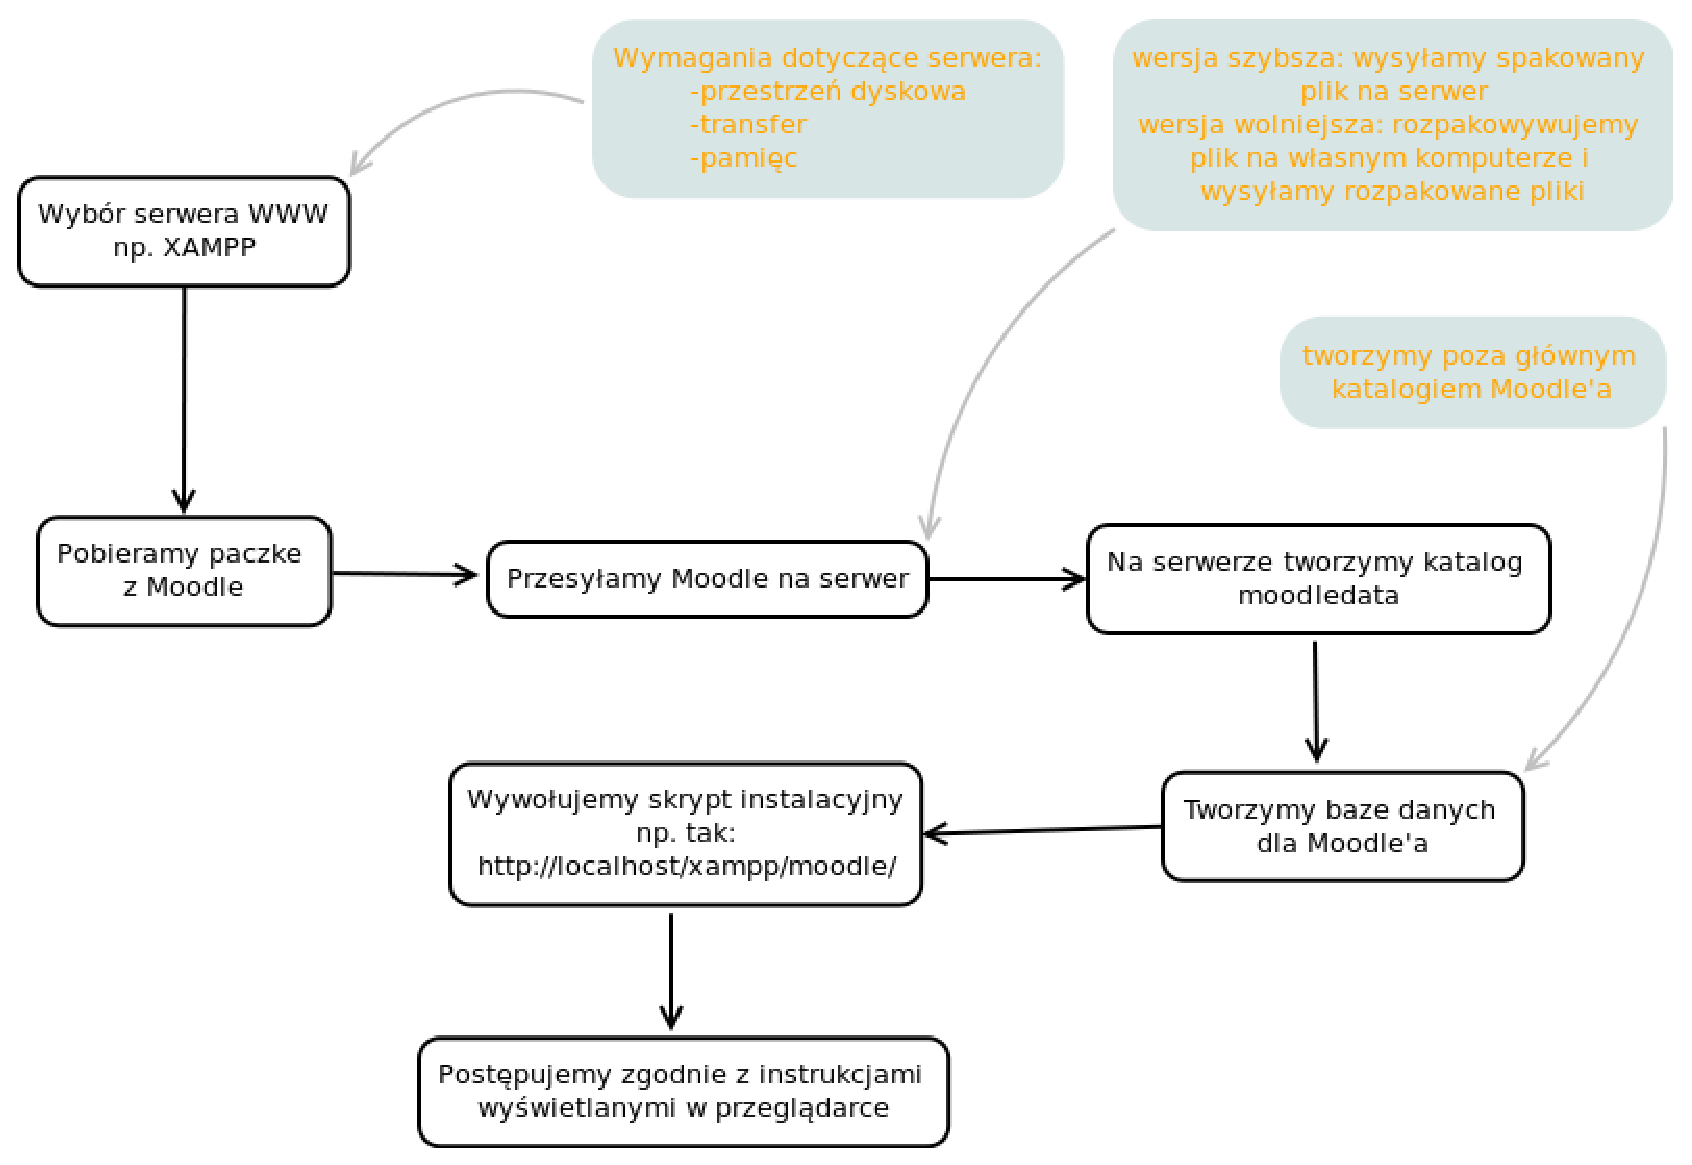
\includegraphics[width=1\textwidth]{projekt_sys//rys//instalacja.eps}
\end{figure}
\begin{figure}[!h]
	\centering
		\caption[Tworzenie kursu]{Schemat blokowy tworzenia nowego kursu} \label{rys:kurs}
		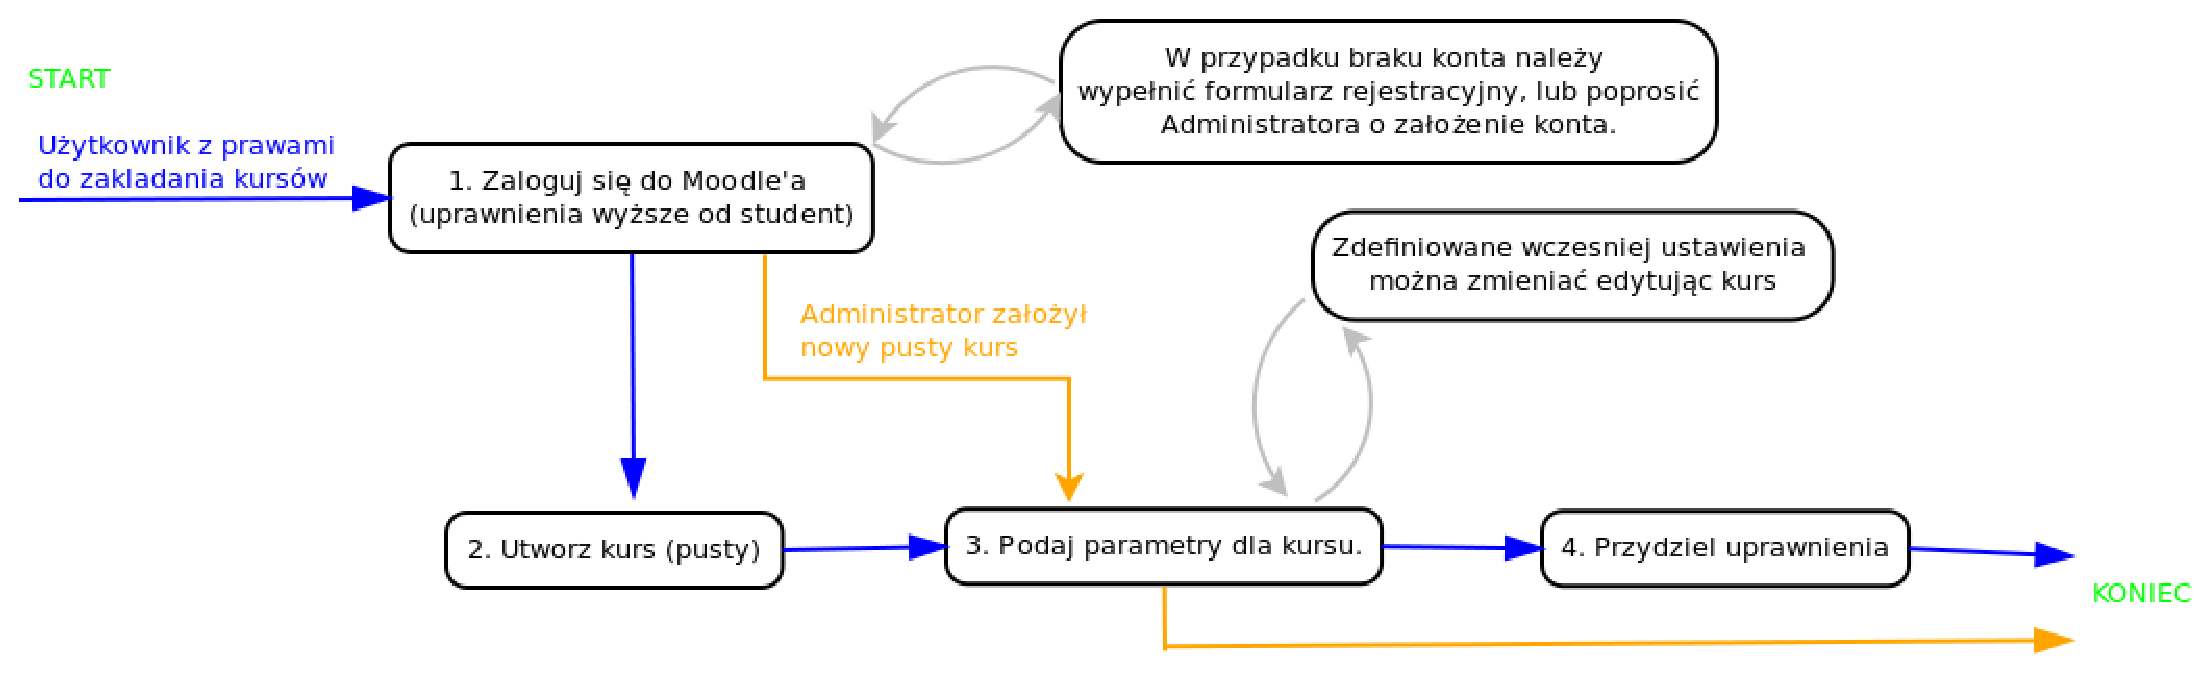
\includegraphics[width=1\textwidth]{projekt_sys//rys//nowy_kurs.eps}
\end{figure}

	\newpage
\chapter{Uwagi końcowe i wnioski} \label{roz:rozdzial_8}
	\thispagestyle{empty}
	\hspace{1cm} Przyglądając się stronie technicznej Moodle'a widać że jego struktura jest taka sama jak ogólna struktura platformy edukacyjnej. Więc aby podsumować i ująć wszystko w kilku słowach możemy powiedzieć, że potrzebny nam serwer, inaczej komputer, który działa przez 24 godziny, jest wpięty do sieci Internet i ma rozpoznawalny adres IP. Następnie musimy mieć zainstalowaną platformę Moodle'a. Cel ten udało się osiągnąć. W tym przypadku skorzystałem z usług hostingowych ze strony \href{http://fazz.pl/}{\textit{http://fazz.pl/}}. Jest to jeden z darmowych hostingów. Na jednym z darmowych kont można śmiało postawić Moodle'a. Proces i plan tworzenia kursu został omówiony w rozdziale wyżej. W projekcie widać, utworzenie prostego kursu nie stanowi żadnego problemu nawet dla laika. Dodawanie materiałów do kursu również nie stanowi większych problemów. Dzięki dobremu interfejsowi platforma Moodle'a jest platformą bardzo intuicyjną. I można samemu idąc drogą eksperymentów stworzyć dobry kurs czy też dobrze przygotowany kawałek materiałów. Mój kurs miał za zadanie przeprowadzić użytkownika przez proces instalacji co udało się zrealizować. \\
\ \\
Platforma Moodle'a jest intuicyjna w obsłudze i została zaopatrzona w przydatny system pomocy, dostępny na oficjalnej stronie \href{http://moodle.org}{\textit{moodle.org}}. Użytkownik znajdzie tam dokładne informacje dotyczące korzystania z każdej funkcji Moodle'a. Do zalet systemu Moodle zalicza się różnorodność zasobów edukacyjnych:
\begin{itemize}
	\item Teksty pisane
	\item Teksty mówione
	\item Animacje
	\item Prezentacje
	\item Rebusy
	\item Hiperłącza
\end{itemize}
Struktura Moodle'a odpowiada potrzebą szkół i uczelni, co widać w sieci. Prawie każda uczelnia posiadająca swoja platformę edukacyjną bazuje ją na Moodle'u. Chociażby nasza politechnika. Która również dla swoich potrzeb wdrożyła dany system. Tworząc kurs korzystamy z pewnych form stworzonych specjalnie pod to zadanie, ale każdy autor kursu decyduje sam o jego specyfice. Autor kursu ma możliwość wprowadzania korekt do działalności, zarówno uczącego się jak i nauczyciela. Tworząc kurs posiadamy różne możliwości zarządzania kursem poprzez takie narzędzia jak:
\begin{itemize}
	\item Lekcje
	\item Warsztaty
	\item Głosowania
	\item Ankiety
	\item Zadania
	\item Fora
	\item Czaty
	\item Opisy
	\item Testy
	\item Dzienniki
\end{itemize}
Na mojej witrynie do zarządzania kursem zostały użyte takie narzędzia jak czaty i fora. Podczas prowadzenia kursów mamy możliwości dodawania dodatkowych materiałów które rozszerzają naszą wiedzę w danym temacie. W kursie mamy również możliwość wielokrotnego powracania do konkretnych treści. Kurs nie przewiduje dzielenia na grupy, które są zbyteczne przy takiej formie kursu, ale istnieje możliwości dzielenia uczniów na grupy. Jest to pomocne w przypadku chęci podzielenia uczniów ze względu na klasy. Witryna posiada również kalendarz który pozwala przypominać użytkownikom o różnych zdarzeniach. Witryna pozwala na śledzenie każdego działania użytkownika, pokazuje operacje jakie wykonał użytkownik przy rozwiązywaniu konkretnych zadań. Mamy również możliwość adaptować zawartość, metody i tempo uczenia się, ze względu na poziom i możliwości uczącego się. Więc można stwierdzić z całą pewnością, że postawiony cel którym było stworzenie przykładowej witryny e-learning-owej wspomagającej zdalne nauczanie został osiągnięty przy pomocy systemu Moodle'a. Pokazuje to, że Moodle stanowi dużą konkurencje i alternatywę dla komercyjnych platform e-learning-owych. Dzięki budowie modułowej jesteśmy wstanie w łatwy sposób tworzyć kursy i dodawać do nich nowe treści. Moodle obserwuje bardzo duży i szybki wzrost użytkowników. I co za tym idzie zwiększa się jego społeczność, gdzie to właśnie ona jest odpowiedzialna za rozwój tej platformy.\\
\ \\
Praca można potraktować jako plan projektu, który można zrealizować. Poszczególne rozdziały dostarczają wiedzy na temat e-learningu oraz jego idei. Pomagają również w podjęciu decyzji zgodnych z postawionym wcześniej celem, które dany użytkownik chce osiągnąć tworząc własną witrynę nauczania. Podczas tworzenia witryny wykonuje się zazwyczaj określona sekwencję kroków, które zostały zaprezentowane w pracy. Poprzez własne eksperymenty można w łatwy sposób wzbogacić swoją witrynę poprzez zwiększenie jej możliwości. Moodle jest platformą która dzięki przyjaznemu interfejsowi zachęca do eksploracji zawartych w systemie funkcji. W pracy dużą część poświęcono na pokazaniu zalet jakie niesie za sobą korzystanie z e-learningu. \\
\ \\
Podczas pisania pracy nie zabrakło i problemów. Jednym z pierwszych problemów było znalezienie darmowego hostingu. Gdyż nie wszystkie darmowe konta spełniają możliwości platformy Moodle'a. Problem ten po większej analizie usług hostingowych został rozwiązany. Następnym krokiem był proces instalacji i konfiguracji platformy, gdzie obyło się bez większych niespodzianek. Proces instalacji w sam w sobie jest zadaniem prostym i nawet ktoś z nie wielką wiedzą informatyczną jest w stanie zainstalować tego typu platformę. Projekt witryny został stworzony jakiś czas temu. Podczas upływającego czasu usługodawca hostingu zmienił serwery. I co za tym idzie zmieniła się darmowa domena dla platformy. Co w znacznym stopniu utrudniło przywracanie backup'u. Po przywróceniu całej platformy należało zmienić ręcznie ścieżki do obrazków czy też innych źródeł zawartych w materiałach. Gdzie bazy danych również musiały być przywracane ręcznie przy pomocy panelu phpMyAdmin i skryptów SQL. Większość prac nad witryną przebiegała sprawnie i nie wymagała dużej ingerencji z mojej strony w kod źródłowy. \\
\  \\
Witrynę możemy rozwijać wedle jakich kol wiek upodobań. Moodle jest systemem z bardzo dużą opcją możliwości. \\
Zacznijmy od sposobów uwierzytelniania, dostępne opcje to:
\begin{itemize}
	\item Uwierzytelnienie z wykorzystaniem poczty elektronicznej (opcja ta jest wykorzystana w projekcie)
	\item Użycie serwera CAS\footnote{CAS~-~Centralny System Uwierzytelniania (ang. Central Authentication Service) CAS to specjalny program. W dużym uproszczeniu służy do pilnowania, gdzie komu w konkretnym systemie informatycznym (lub ich zbiorze) wolno zajrzeć. Sam CAS nie przechowuje jednak danych użytkowników, takich jak hasła. Musi współpracować z jakimś zbiorem informacji o użytkownikach.}.
	\item Zewnętrzna baza danych
	\item Użycie serwera IMAP\footnote{IMAP~-~(ang. (Internet Message Access Protocol) jest protokołem warstwy aplikacji w architekturze protokołów Internetowych. Jego głównym zadaniem jest umożliwienie stacji roboczej dostępu do listów elektronicznych znajdujących się w skrzynce pocztowej na serwerze pocztowym. }
	\item Użycie serwera LDAP\footnote{LDAP~-~(ang. Lightweight Access Directory Protocol) serwer usług katalogowych.}.
	\item Moodle Network authentication.
	\item Użycie serwera NNTP\footnote{NNTP~-~(ang. Network News Tranport Protocol), jak nazwa wskazuje jest protokołem "na którym" działają niusy.}
	\item Brak uwierzytelniania.
	\item PAM\footnote{System uwierzytelniania w systemie Linux wykorzystuje mechanizm PAM (Pluggable Authentication Modules - Dołączalne Wtyczki Uwierzytelniające). Implementację dla systemu Linux stworzył i cały czas rozwija Andrew G.Morgan. System PAM to zestaw bibliotek i wtyczek, które są wykorzystywane do uwierzytelniania użytkowników w systemie. Biblioteka jest wykorzystywana przez aplikację, aby wywołać procedurę uwierzytelniającą. Wtyczki określają możliwości systemu uwierzytelniającego, możliwościami taki są ograniczenie czasu logowania do konkretnych godzin, określenie różnych źródeł danych o użytkownikach (na przykład baza LDAP, MySQL i inne). }.
	\item Użycie serwera POP3\footnote{POP3~-~Post Office Protocol version 3 to protokół internetowy z warstwy aplikacji pozwalający na odbiór poczty elektronicznej ze zdalnego serwera do lokalnego komputera poprzez połączenie TCP/IP. Ogromna większość współczesnych internautów korzysta z POP3 do odbioru poczty.}.
	\item Użycie serwera RADIUS\footnote{RADIUS~-~(ang. Remote Authentication Dial In User Service), usługa zdalnego uwierzytelniania użytkowników. Protokół używany do uwierzytelniania. Stosowany przez dostawców internetowych na serwerach innych niż serwery z systemem Windows. Obecnie jest najpopularniejszym protokołem podczas uwierzytelniania i autoryzowania użytkowników sieci telefonicznych i tunelowych.}.
	\item Shibboleth\footnote{Shibboleth~-~działa jako servlet, sam nie przechowuje danych, pobiera je z innych źródeł np. LDAP}
\end{itemize}
Następnym rozwinięciem czy też zmianą naszego projektu jest zmiana wyglądu. Wygląd witryny możemy zmieniać poprzez stworzenie własnego design, lub też skorzystanie z już dostępnych kompozycji. Aby zmienić wygląd należy skorzystać z bloku \textbf{Administracja serwisu}, a następnie 
\begin{verbatim}
	Wygląd->Tematy->Wybór kompozycji.
\end{verbatim}
Do witryny możemy dodawać dowolnej treści kursy. Poprzez tworzenie większej ilości kursów nasza witryna będzie się rozwijała i powiększała swoją liczbę użytkowników. \\
Podsumowując, witrynę zbudowana na podstawie systemu Moodle'a daje nam bardzo dużą możliwość działania. Wygląd i ustawienia witryny głównie zależą tylko i wyłącznie od administratora. On decyduje jakie procesy i jakie kursy będziemy mogli włączać do naszej platformy aby zwiększyć atrakcyjność naszej witryny.\\
\\
Tworząc witrynę z kursem pokazującym jak zainstalować i skonfigurować Moodle'a, pierwszym etapem jaki wykonałem po zainstalowaniu Moodle'a, była jego konfiguracja. W początkowej fazie konfiguracji zająłem się sposobem rejestracji użytkownika do systemu. Wybrałem funkcje uwierzytelniania z wykorzystaniem poczty elektronicznej plus korzystanie z serwisu \textit{reCAPTCHA}. Aby system współdziałał z \textit{reCAPTCHA} należy na stronie \href{http://recaptcha.net}{\textit{http://recaptcha.net}} wygenerować dla danej strony klucz publiczny i klucz prywatny, a następnie przejść do \textit{Administracja serwisu/Użytkownicy/Uwierzytelniania/Zarządzaj uwierzytelnianiem} i w odpowiednich polach podać wygenerowane klucze. Również dodatkową opcją z której skorzystałem tworząc witrynę było skonfigurowanie współpracy z narzędziem \textit{GeoIP}. Dodanie tej usługi zacząłem od utworzenia w folderze \textit{moodledata} katalogu \textit{geoip} i podaniu ścieżki dostępu do pliku. W moim przypadku ścieżka dostępu wyglądała tak \textit{/home/nonus25/domains/moodledata/geoip/GeoLiteCity.dat}. Gdzie należy umieścić uprzednio pobrany plik \textit{GeoLiteCity.dat} z adresu\\ \href{http://www.maxmind.com/download/geoip/database/GeoLiteCity.dat.gz}{\textit{http://www.maxmind.com/download/geoip/database/GeoLiteCity.dat.gz}}. Następnie przeszedłem do strony \href{http://code.google.com/apis/maps/signup.html}{\textit{http://code.google.com/apis/maps/signup.html}} gdzie wygenerowałem API klucz dla \textit{Google Maps} podając swoją domenę \href{http://moodle.chmielua.fazz.pl}{\textit{http://moodle.chmielua.fazz.pl}}. Wygenerowany klucz należy wpisać w odpowiednie pole znajdujące się na stronie\\ \textit{Administracja serwisu/Lokalizacja/Ustawienia lokalizacji}. Więcej na temat moich prac jakie wykonywałem tworząc witrynę znajduje się w rozdziale \textit{Projekt systemu~-~Konfiguracja witryny}. Kompozycja wyglądu platformy została pobrana przez zemnie ze strony \\ \href{http://moodle.org/mod/data/view.php?d=26}{\textit{http://moodle.org/mod/data/view.php?d=26}}. Pobrany pakiet należy umieścić w katalogu \textit{themes}. W pobranej kompozycji dokonałem kilku zmian zamieniając główną ikonę platformy (jest to ikona znajdująca się w katalogu \textit{themes/custom\_corners/favicon.ico}), oraz dokonałem zmiany domyślnego obrazka dla użytkownika. W kodzie źródłowym dokonałem małych zmian co do wyglądu nagłówka jak i stopki strony. Są to pliki znajdujące się \textit{themes/custom\_corners/}. Za nagłówek strony odpowiedzialny jest plik \textit{header.html} gdzie dodałem swój kawałek kodu 
\begin{verbatim}
<img  class="headermain" 
src="http://moodle.chmielua.fazz.pl/images/moodle/eLearningLogoTag-sm.png" 
alt="E-learning moodle.chmielua.fazz.pl" 
/>
\end{verbatim}
i za komentowałem kod odpowiadający za wyświetlanie napisu w tym miejscu 
\begin{verbatim}
<!-- <h3 class="headermain" color><?php echo $heading ?></h3> -->
\end{verbatim}
w dwóch lokalizacjach:
 \begin{verbatim} <?php print_container_start(true, '', 'header-home'); ?>
<?php print_container_end(); ?>\end{verbatim}
oraz
\begin{verbatim}<?php print_container_start(true, '', 'header'); ?>
<?php print_container_end(); ?>\end{verbatim}
Za stopkę witryny odpowiedzialny jest plik \textit{footer.html} gdzie moje zmiany wyglądały w następujący sposób:
\begin{verbatim}
    print_container_start(false, '', 'footer');
    echo '<p class="helplink">';
    //echo page_doc_link(get_string('moodledocslink'));
    echo '<a href="http://chmielua.blogspot.com/search/label/Moodle">
	Trochę inaczej o Moodle</a>';
    echo '</p>';
   
    //echo $loggedinas;
    echo '<img src="http://moodle.chmielua.fazz.pl/
		images/moodle/elearning_logo.png" />';
    //echo $homelink;\end{verbatim}
Dokonałem również zmiany układu strony, aby zmienić układ kolumn na stronie należy dodać następującą kod w pliku \textit{config.php}, 
\begin{verbatim}
$THEME->layouttable = array('middle', 'right', 'left');
\end{verbatim}

	\newpage

% ********************* Bibliografia *********************
\begin{thebibliography}{99}
	\bibitem{dokumentacja_moodle} Dokumentacja~Moodle'a \\
	\textit{\href{http://docs.moodle.org/pl/O\_Moodle}{http://docs.moodle.org/pl/O\_Moodle}} \\
	\textit{\href{http://docs.moodle.org/pl/Instalacja\_Moodle}{http://docs.moodle.org/pl/Instalacja\_Moodle}}
	\bibitem{wiki_e-l} E-Learning Wikipedia \\
	\textit{\href{http://pl.wikipedia.org/wiki/E-learning\#Podej.C5.9Bcia\_pedagogiczne}{http://pl.wikipedia.org/wiki/E-learning\#Podej.C5.9Bcia\_pedagogiczne}}
	\bibitem{pedagogika}  Kształcenie na odległosc na podstawie wykorzystania \\systemu CLMS MOODLE jako technologia pedagogiczna\\
	\textit{\href{http://www.up.krakow.pl/ktime/ref2007/Smyrnova.pdf}{www.up.krakow.pl}}
	\bibitem{nowakowski} Z.~Nowakowski. \textit{Nowe koncepcje kształcenia oparte na e-learning},\\CKPiDN w Mielcu, \textit{"Zeszyty nauczycielskie"}, 2005
	\bibitem{moodle_test} \textit{Moodle 1.9 Testing and Assessment} Jason Myrick
	\bibitem{moodle_multimedia} \textit{Moodle 1.9 Multimedia} João Pedro Soares Fernandes
	\bibitem{moodle_teaching} \textit{Moodle 1.9 Teaching Techniques} William Rice, Susan Smith Nash
	\bibitem{tworzenie_serwisow} \textit{Moodle 1.9 E-Learning Course Development} William H. Rice IV
	\bibitem{use_moodle} \textit{Using Moodle, 2nd Edition} Jason Cole, Helen Foster \textbf{\textit{O'REILLY}}
\end{thebibliography}
\addcontentsline{toc}{chapter}{Bibliografia}
% ********************* Tworzy spis rysunków *********************
	\listoffigures
	\addcontentsline{toc}{chapter}{Spis Rysunków}
% ******************** Tworzy spis tabel *************************
	\listoftables
	\addcontentsline{toc}{chapter}{Spis Tabel}
\end{document}
